\documentclass[preprint,11pt,authoryear]{elsarticle}
\usepackage{amsmath}
\usepackage[font=sf, labelfont={sf,bf}, margin=0cm]{caption}
\usepackage[inline]{enumitem}
\usepackage{epstopdf}   
\usepackage[margin=1in]{geometry}
\usepackage{lineno}
\usepackage{placeins}
\usepackage{subcaption}
\usepackage[usenames,dvipsnames]{color}
\usepackage[usenames,dvipsnames,svgnames,table]{xcolor}
\usepackage{algorithm}
\usepackage{algpseudocode}
\usepackage{textcomp}
\usepackage{graphicx}
\usepackage{tabulary}
\usepackage{float}
\usepackage[utf8]{inputenc}
\usepackage{nomencl}
\usepackage[font=sf, labelfont={sf,bf}, margin=0cm]{caption}  % Margin similar to Anik
\usepackage{placeins}
\usepackage[margin=1in]{geometry}
\usepackage{hyperref}
\usepackage[english]{babel} 
\usepackage{multirow}
\usepackage{nomencl}
\makenomenclature
\definecolor{listinggray}{gray}{0.95}
\definecolor{darkgray}{gray}{0.7}
\definecolor{commentgreen}{rgb}{0, 0.4, 0}
\definecolor{darkblue}{rgb}{0, 0, 0.4}
\definecolor{middleblue}{rgb}{0, 0, 0.7}
\definecolor{darkred}{rgb}{0.4, 0, 0}
\definecolor{brown}{rgb}{0.5, 0.5, 0}

\usepackage[normalem]{ulem}
\makeatletter
\def\cyanuwave{\bgroup \markoverwith{\lower3.5\p@\hbox{\sixly \textcolor{cyan}{\char58}}}\ULon}
\def\reduwave{\bgroup \markoverwith{\lower3.5\p@\hbox{\sixly \textcolor{red}{\char58}}}\ULon}
\def\blueuwave{\bgroup \markoverwith{\lower3.5\p@\hbox{\sixly \textcolor{blue}{\char58}}}\ULon}
\font\sixly=lasy6 % does not re-load if already loaded, so no memory problem.
\makeatother

\newif\ifdraft
\drafttrue
\ifdraft
\usepackage{xcolor}
\definecolor{ocolor}{rgb}{1,0,0.4}
\newcommand{\terminology}[1]{ {\textcolor{red} {(Terminology used: \textbf{#1}) }}}
\newcommand{\jwave}[1]{ {\reduwave{#1}}}
\newcommand{\jhanote}[1]{ {\textcolor{red} { ***shantenu: #1 }}}
\newcommand{\csnote}[1]{ {\textcolor{blue} { ***chaitanya: #1 }}}
\definecolor{orange}{rgb}{1,.5,0}
\definecolor{dandelion}{cmyk}{0,0.29,0.84,0}
\newcommand{\gpnote}[1]{{\textcolor{green} {***giannis: #1}}}
\newcommand{\note}[1]{ {\textcolor{magenta} { ***Note: #1 }}}
\else
\newcommand{\terminology}[1]{}
\newcommand{\jwave}[1]{#1}
\newcommand{\jhanote}[1]{}
\newcommand{\csnote}[1]{}
\newcommand{\gpnote}[1]{}
\newcommand{\note}[1]{}
\fi



\journal{Chemical Engineering Research and Design}
\begin{document}
\begin{frontmatter}

\title{A parallel unidirectional coupled DEM-PBM model for the efficient solution and simulation of 
computationally  intensive systems.}
\author[add1]{Chaitanya Sampat\corref{cor1}}
\author[add1]{Franklin Bettencourt\corref{cor1}}
\author[add1]{Yukteshwar Baranwal}
\author[add2]{Ioannis Paraskevakos}
\author[add1]{Anik Chaturbedi}
\author[add1]{Subhodh Karkala}
\author[add2]{Shantenu Jha}
\author[add1]{Rohit Ramachandran}
\author[add1]{Marianthi Ierapetritou\corref{cor2}}
\address[add1]{Department of Chemical and Biochemical Engineering, Rutgers, The State University of New
Jersey, Piscataway, NJ, USA-08854}
\address[add2]{Electrical and Computer Engineering, Rutgers, The State University of New Jersey, 
Piscataway, NJ, USA-08854}
\cortext[cor1]{Equal contribution by C. Sampat and F. Bettencourt}
\cortext[cor2]{Corresponding author}
\ead{marianth@soe.rutgers.edu}

\begin{abstract}
Particulate processes are prevalent in the pharmaceutical industry but, the
physics underlying these processes are complicated and requires large amount
of computation to solve a model at the particle-level. This approach makes the
simulation slow, when compared to using a less accurate bulk model. A quicker
and a more accurate way to model this system is to use a multi-scale model
i.e. use the particle-scale data into a bulk model. In this work, a
unidirectional multi-scale model was used to model the high shear wet
granulation process. A multi-dimensional population balance model (PBM) was
developed which consisted of a mechanistic kernel, which in turn obtained the
collision data from the discrete element modeling (DEM) simulation. The PBM
was run in parallel using MPI + OMP hybrid technique. The DEM simulations were
performed on LIGGGHTS, which runs in parallel using MPI. Speedup of about 14
times was obtained for the PBM simulations and around 12 for the DEM
simulations. This coupling was performed using the radical pilot for scaling
studies from 1 to 128 cores for the PBM and up to 256 cores for the DEM. Using
this developed framework, the granulation process has been modeled accurately
much faster than existing approaches in literature. \jhanote{Which figure
speaks to the accuracy? Why does the accuracy arise?}
\end{abstract}
\begin{keyword}
Population balance model \sep Granulation \sep Discrete element methods  \sep MPI and OpenMP 
\sep Pharmaceutical process design
\end{keyword}
\end{frontmatter}
\linenumbers

\section{Introduction \& Objectives} 
Half of all industrial chemical production is typically performed via the
processing of particulate systems~\citep{seville1997}. These processes account
for about 70\% of the products of industries like detergents, aerosols,
fertilizers, and pharmaceuticals~\citep{Litster2016}. These processes are
widely popular as these particulate products have great advantages over liquid
formulations such as better chemical and physical stability and reduced
transportation cost. Despite the prevalence of these particulate processes,
the underlying physics of these processes is poorly
understood~\citep{Rogers2013}. As a result industries that rely on these
processes, especially pharmaceuticals, have to use expensive heuristic studies
and inefficient operational protocols with high recycle ratios to meet strict
regulatory standards~\citep{Ramachandran2009}. This can drive up the costs and
delay the release of new products. What makes these processes so challenging
to design is that there are none or few governing equations to accurately
predict their behavior~\citep{sen2013}.

Particulate processes are defined by chaotic micro-scale phenomena that result
from the many particle-particle interactions inside these systems. These small
scale phenomenon develop into complex bulk behavior of these processes. To
successfully predict the bulk behavior of these systems, a model needs to
capture the particle-particle interactions and emergent meso-scale phenomena.
Recently, the Discrete Element Method (DEM)~\citep{Cundall1979} simulations
have been employed in pharmaceutical process modeling to obtain particle-level
data, which helps describe the bulk properties of the particulate system
accurately~\citep{Hancock2011}. DEM uses Newton's equations of motion to model
the forces on each particle in the system and it's interactions with the
system geometry and other particles. This enables DEM to model the small scale
phenomena that determines the bulk behavior of particulate system. Since DEM
includes large amount of interactions and force computations, it usually takes
a large amount of time to run. Thus, there is a need for a more efficient
simulation technique for these particulate particles. One of the common
methods used in the industry is the population balance model (PBM), which is
more computationally efficient but, lacks the accuracy of the DEM.

PBM takes into account the changes in internal or spatial particle
properties.This model lacks sensitivity to design parameters such as equipment
geometry. It is semi-mechanistic in nature, meaning they use population
averages and probability to capture bulk behavior but still seek to capture
some of the micro-phenomena of particle-particle interactions using
correlations or empirically developed kernels to approximate those
interactions. Even though PBM is much faster than DEM, a detailed PBM can
still take a significant amount of time to solve which prevents them from
being used as widely as they could be in academia and industries
\citep{Barrasso2013}. Though highly detailed PBMs take into account
populating, averaging and contain semi-mechanistic kernels, these PBMs still
can have difficulties in capturing the micro-scale phenomena that are crucial
to predicting accurate dynamics of particulate processes.

Thus, to complement the limitations of each of these modeling techniques they
are coupled to provide a more accurate model.  The typical work flow of such a
PBM-DEM coupled model involves using a short DEM simulation to capture the
particle-particle level interactions of the system and then this physics is
fed into the PBM, so that the PBM can more accurately simulate bulk system
behavior~\citep{Goldschmidt2003}~\citep{Reinhold2012}~\citep{Barrasso2013}.
This PBM-DEM method is more accurate than a PBM simulation alone but runs much
faster than a complete DEM simulation. Despite the performance benefits of
these coupled PBM-DEM models they still take unacceptably long to solve. In
the past high-oerformance computing (HPC) has been used to speed up computationally
intensive problems such as Molecular Dynamics (MD), Computational Fluid
Dynamics (CFD) and in recent years  this technique has been applied to DEM and
PBM
simulations~\citep{Bettencourt2017}~\citep{Prakash2013a}~\citep{Gunawan2008}.

\jhanote{Parallel computing is a type/subset of high-performance computing
(HPC). Please use HPC rather than parallel computing. Also need consistency of
usage; see next paragraph.} \csnote{have changed the occurence parallel computing to HPC}


Parallel Computing is the standard procedure to solve large computational
problems in many sciences. \jhanote{What is this a reference to?} This method
uses High Performance Computing (HPC) systems \jhanote{HPC = High-peformance
computing, not computers} \csnote{Have addressed the name} to solve over a large number of cores. A HPC
consists of thousands of compute nodes connected via a high speed network. A
typical compute node has multiple cores and several GBs or memory. The network
that connects them, usually Infiniband, reaches speeds of 56 Gbps. In
addition, a high performance parallel filesystem accompanies the compute
nodes, allowing users to read and write GBs of data efficiently. One of the
challenges when implementing parallel applications is to make sure that data
is written in a similar manner to serial programs. To ensure correctness of
the results, an appropriate data communication implementation is required.
\jhanote{the above should not be in the introduction. GET to the message
of the contribution of this work, not background/related work.}


Some of the benefits of using HPC in the pharmaceutical industry include high
accuracy for parameter estimation as detailed particle-scale simulations can
be performed quickly. Quick simulations can also help improve control of
continuous pharmaceutical processes. This work showcases the speed
improvements that can be achieved using HPCs and how they can help improve
process design. \jhanote{All of this can come later. Get to the problem this paper
is addressing, the solution/approach and specific contribution. You've alread
irritated the reviwer and reader by now} 
\csnote{Will be replacing the above paragraph with the one below.}

Product quality is of prime importance when it comes to the pharmaceutical 
products. Thus, the model implemented to control the system should be fast 
enough to predict the deviation and correct it before the product 
quality is affected. DEM and PBM are used to model granulation which take 
a large amount of time to simulate. This arises the need to increase speed 
of the simulation such that this process can be controlled online. 
To apply the corrective actions, parallel versions of these codes need to be run 
on large number of cores. This infrastructure is usually found on a supercomputer 
making HPC systems a major component for the online control of such system.

\jhanote{What is the specific engineering problem you are interested in
solving that cannot be solved without HPC? It is unclear to the reader.} The
main objective of this work is to develop a unidirectional DEM-PBM model that
runs efficiently in parallel so that it can take advantage of the
computational capabilities of  modern computing clusters. In the course of
development of the model, the DEM simulation were performed on LAMMPS Improved
for General Granular and Granular Heat Transfer simulations
(LIGGGHTS)~\citep{Kloss2012} to model the micro-mechanics of the L\"{o}dige
CoriMix CM5 high shear granulator. A 4-Dimensional, reduced order DEM informed
PBM was developed that is parallelized using hybrid techniques (Message
Parsing Interface (MPI) + Open Multi-Processing (OMP))to model the bulk
processes occurring during the granulation process and is discussed in
section~\ref{sec:pbm_model}. Section~\ref{sec:RPandCommunications} describes
unidirectional coupling of DEM and PBM using Radical Pilot, which is a
framework developed in Python. This provides task level parallelization, to
help develop an accurate model which can be run quickly on high performance
computing systems. The speed improvements obtained for the parallel code and
further improvements that can be implemented are discussed in
Section~\ref{sec:Results}


\section{Background \& Motivation}

\subsection{Particulate processes}
Particulate processes are ones in which a system of discrete species exist,
such as granules or catalyst pellets, that undergo changes in average
composition, size, or other pertinent properties. Granulation is one such
particulate process which is commonly found in the pharmaceutical industry. In
this process, fine powders are converted to larger granules using a liquid
binder. The three rate processes governing granulation are wetting and
nucleation, consolidation and aggregation and attrition and
breakage~\citep{Iveson2001}~\citep{Cameron2005}. As the liquid is added to the
fine powder, it forms a porous nuclei that can coalesce, deform and
break~\citep{Barrasso2015ces}. As there is an alteration in the properties of
these nuclei, they can take up additional liquid or breakdown to a finer
powder.To understand how a granulation processes will behave with different
design and operating parameter settings and formulations, experimental studies
are performed which is a method referred to as Quality-by-Testing (QbT). This
methodology is time consuming and expensive. Thus, newer research is focused
on the QbD concept i.e, developing a mathematical model to represent the rate
process.

\subsection{Modeling}
The paradigm shift of the pharmaceutical industry for instance towards
continuous manufacturing, emphasizes the need for a more accurate model. This
further helps to develop better control strategies for the process. The
modeling of particulate processes is more time consuming and computationally
expensive when compared to fluid systems since particles are considered as
individual entities rather than a continuum like fluid systems. The models
discussed ahead represent the particle-particle interaction at meso and micro-
scale.
\subsubsection{Discrete Element Modeling (DEM)}
 Discrete Element Method is a simulation technique used to monitor the
behavior of each particle as a separate entity compared to other bulk
continuum models. This method tracks the movement of each particle within the
space, records the collisions of each particle with the geometry as well as
with each other and it is also subject to other force fields like
gravity~\citep{Barrasso2015cerd}. This model is based on the Newton's laws of
the motion as shown in Equations~\ref{eqn:bkgd_dem_n2law} \&
\ref{eqn:bkgd_dem_forcebal} : \\
\begin{align}
m_i\frac{dv_i}{dt} &= F_{i,net} \label{eqn:bkgd_dem_n2law} \\
F_{i,net} &=  F_{i,coll} +  F_{i,ext} \label{eqn:bkgd_dem_forcebal}
\end{align}
Where, $m_i$ is the mass of the particle, $v_i$ represents the velocity of the
particle, $F_{i,net}$  represents the net force on the particle, forces on the
particle due to collisions and other external forces are represented in
$F_{i,coll}$ and $F_{i,ext}$ respectively.

Using this method, the distance between each particle is calculated at every
time step and if the distance between two particles is less than the sum of
the radii (for spherical particles)  a collision between the two particles is
recorded. The tolerance for overlap is low in the normal as well as the
tangential direction. Micro-scale DEM simulations are computationally
demanding and simulations may take up to several days to replicate a few
seconds of real time experiments. Many methods have been implemented to
increase the speed of these simulations, such as scaling by increasing the
size of the particles. These approximations are good in understanding the
physics of the system but are not directly applicable to process-level
simulations.

The particle-particle collisions are not always elastic, thus there is a need
for models for the contact forces. The earliest elastic model was developed by
Hertz and was extended by Mindlin by accounting for the  tangential forces
during the collisions~\citep{adams2000}. The Hertz-Mindlin contact
model~\citep{gantt2006}~\citep{hassanpour2013} has been utilized in this work.
 

\subsubsection{Population Balance Model (PBM)}
     Population balance models (PBM) predict how groups of discrete entities will behave on a 
    bulk scale due to certain effects acting on the population with respect to time~\citep{ramkrishna2014}. In the context of process engineering and granulation, population 
    balance models are used to describe how the number densities, of different types of particles, in 
    the granulator change as rate processes such as aggregation and breakage reshape particles~\citep{Barrasso2013}. A general form of population balance model is shown in Equation~\ref{eqn:bkgd_pbm_general}.
    
    \begin{align}
    \frac{ \partial}{\partial t}F(\textbf{v},\textbf{x},t) +& \frac{\partial}{\partial 
        \textbf{v}}[F(\textbf{v},\textbf{x},t)\frac{d\textbf{v}}{dt}(\textbf{v},\textbf{x},t)] + 
    \frac{\partial}{\partial \textbf{x}}[F(\textbf{v},\textbf{x},t)\frac{d\textbf{x}}{dt}(\textbf{v},\textbf{x},t)] 
    \notag\\
    &= 
    \Re_{formation}(\textbf{v},\textbf{x},t)+\Re_{depletion}(\textbf{v},\textbf{x},t)+\dot{F}_{in}(\textbf{v},
    \textbf{x},t)-\dot{F}_{out}(\textbf{v},\textbf{x},t)
    \label{eqn:bkgd_pbm_general} 
    \end{align}
    
In Equation~(\ref{eqn:bkgd_pbm_general}), $\textbf{v}$ is a vector of internal coordinates. For 
modeling a granulation process $\textbf{v}$ is commonly used to describe the solid, liquid, and gas 
content of each type of particle. The vector $\textbf{x}$ represents external coordinates, usually 
spatial variance. For a granulation process this  account for spatial variance in the particles as they 
flow along the granulator.

\subsubsection{Coupled DEM-PBMs}
The use of multi-physics models has recently been adapted to understand the behavior of 
particle systems. These models help understand the physics of the system at various scales 
\textit{i.e.} micro, meso and macro scale~\citep{sen2014}. Particle process dynamics have been 
inferred from coupling of various physics models \textit{viz.} CFD, 
DEM and PBM. Earlier works from \cite{sen2014} \& \cite{Barrasso2015cerd} have successfully 
predicted process dynamics of the granulation process using such multi-physics models.

Initially, \cite{ingram2004} coupled PBM and DEM using two different multi-scale frameworks which 
focused on methods of integration and information exchange required between these two methods. 
Later efforts on coupling of PBM and DEM were unidirectional in nature, where the collision 
data was obtained from the DEM and then used it in PBM. \cite{gantt2006} used the DEM data 
to build a mechanistic model for the PBM. \cite{Goldschmidt2003} solved a PBM using DEM by 
replacing smaller particles as they successfully coalesce with larger particles. 
\cite{Reinhold2012} replaced a mechanistic aggregation kernel with an empirical kernel 
in order to prove that, in certain cases DEM simulations may not be necessary for the 
development of kernels. A hybrid model for one-way coupling has been reported for continuous mixing~\citep{sen2013}~\citep{sen2013b} and is discussed in Section \ref{sec:pbm_model}.

In this work, a coupled DEM and PBM model has been implemented. In general, the PBM provides meso-scale 
information while the DEM gives particle scale information. The combination of these two methods helps 
describe the process dynamics with more accuracy. However, calculations involved due to the number 
of particles involved in the DEM process as well as PBM become computationally very heavy, hence the
motivation and need for running the simulations on HPCs and parallelization techniques. 
 

\subsection{Parallel computing and computer architectures}

\subsubsection{Computer Architecture}

\jhanote{HPC has been defined. Please use it} \csnote{Changed}

Analogous to a conventional PC a HPC cluster node has
one or more CPUs and RAM. Commonly nodes are manufactured with two CPUs, each
CPU is a multi-core meaning it has multiple compute cores such that each can
carry out calculations separately from one another. On a node, memory is
divided by CPU sockets, so each CPU has direct access to memory that is local
to its own socket, however accessing memory on another socket is much
slower~\citep{Jin2011}. For this reason. data that is needed for computation
should be stored locally to the CPU that needs it.

There are two classes of computer architecture which can be classified by
memory locality features such as distributed memory systems or shared memory
systems. These two classes co-exist in a cluster, thus providing the benefits
of each. All the nodes exchange memory using explicit message passing while
each has its own independent memory. The cores on each node can access data
from the shared memory without any explicit message passing statements from
the user. While designing a parallel program all these aspects need to be
considered for optimal performance of the code~\citep{Adhianto2007}.


\subsubsection{Parallel application programming interfaces}
Message Passing Interface (MPI) is a common parallel computing application 
programming interface standard. MPI is used for distributed memory parallel computing and this is 
because the application programming interface will operate 
every MPI process as a discrete unit that does not share memory with the other processes unless explicit 
message passing is used. Even on shared a single node where the hardware supports shared 
memory computing, MPI will still operate it in a distributed memory fashion~\citep{Jin2011}. Operating all 
cores as distinct units also means they each need their own copy of all variables used for computation 
which results in a large overall memory foot print compared to a similar system if it was operated in 
shared memory. 

Open Multi-Processing (OMP) is another application program interface stand for parallel 
computing. OMP is used for shared memory and can take advantage of shared memory systems which 
can result in much faster computation. Although, it does not work well on distributed systems. This 
prevents it from being used to efficiently carry out computations across multiple nodes of a cluster 
simultaneously~\citep{Jin2011}. 

Since MPI is preferred for distributed computing and OMP is better for shared computing many 
researchers have studied the performance of MPI vs MPI+OMP methods. Many a times a trade off is made 
between optimizing a program for performance and trying to make it flexible enough to run on many 
different computer architectures. It was found that hybrid methods for PBMs allow the code 
flexibility for different architectures while still maintaining good performance~\citep{Bettencourt2017}.  
It was also reported that only the external(spatial) coordinates of the PBM were parallelized. 
In this current work external and internal(compositions) calculations are parallelized. 

\subsubsection{Previous works on parallel development and solution of PBM and DEM}
The idea of parallelization to reduce the computation time of the DEM and PBM simulations have 
been employed by various researchers in the past. \cite{Gunawan2008} used high-resolution 
finite volumes solution methods for the parallelization of their PBM. They performed load 
balancing effectively by decomposing the internal coordinates of their PBM. They achieved 
speed improvements up to 100 cores on one system size, but was not tested for models 
with more dimensions. Moreover, they mentioned that parallelization could be 
improved using shared memory processing. 
In our previous work, \cite{Bettencourt2017} took a 
hybrid approach towards the parallelization of the PBM using both MPI and OMP. 
The hybrid parallelization helped achieve a speed improvement of about 98\% using 
128 cores over the serial code. 
\cite{Prakash2013a} \& \cite{Prakash2013b} used the inbuilt Parallel Computation 
Toolbox (PCT) in MATLAB~\citep{pctMatlab} to parallelize their PBM on lower number 
of cores, but this faced the shortcomings of MATLAB's internal processing and 
could not achieve the speed improvements of parallelization of a program if 
it were written in a native programming language like C/C++ or FORTRAN. 

LIGGGHTS~\citep{Kloss2012}, an open-source software used to perform DEM simulations has native 
support for MPI for parallelizing the simulation by static decomposition which partitions space such that 
the area of communication between the the MPI processes is minimized. \cite{kacianauskas2010} used 
load balancing methods similar to a static decomposition and observed that this works well for a 
mono-dispersed system but the computational effort increases for simulations for poly-dispersed 
material. \cite{Gopalakrishnan2013} also reported a speed increase and a parallel efficiency of about 
81\% in their CFD-DEM simulation. LIGGGHTS could not take advantage of shared memory interfaces 
since it did not support OMP. \cite{Berger2015} implemented hybrid parallelization methods for the 
particle-particle interaction and the particle-wall interaction modules in LIGGGHTS and also used the 
Zoltan library~\citep{Boman2012} developed by Sandia National Laboratories for dynamic load 
balancing. They achieved a speed improvement of about 44\% for simulations performed on higher 
number of cores, but there was no significant speed improvement for smaller core counts. 

\subsection{Pilot abstraction and RADICAL-Pilot (RP)}
A primary challenge faced is the scalable execution of multiple (often two,
but possibly more) heterogeneous simulations that need to run independently
but have a need to communicate and exchange information. Traditionally each
simulation is submitted as an individual job, but that invariably leads
to a situation where each simulation gets through the batch-queue systems
independent of the other. So although the first-through-the-queue is ready to
run, it stalls fairly soon waiting for the other simulation to make it through
the queue.  On the other hand MPI capabilities can be used to  execute both
simulations as part of a single multi-node job.  Thus whereas the former
method suffers from unpredictable queue time for each job, the latter is
suitable to execute tasks that are homogeneous and have no dependencies.


The Pilot abstraction~\citep{pstar12} solves these issues:  The Pilot abstraction 
(i) uses a container-job as a placeholder to acquire resources, and (ii) decouples 
the initial resource acquisition from task-to-resource assignment. Once the 
Pilot (container-job) has acquired the resources, it can be populated with 
computational tasks. This functionality allows all tasks to be executed directly 
on the resources, without being queued individually. Thus, this approach supports 
the requirements of task-level parallelism and high-throughput as needed by 
science drivers.


RADICAL-Pilot is an implementation of the Pilot abstraction in Python, engineered to
support scalable and efficient launching of heterogeneous tasks across different platforms.
\section{Methods}

\subsection{Discrete Element Method (DEM)}
\subsubsection{LIGGGHTS}
LAMMPS Improved for General Granular and Granular Heat Transfer simulations (LIGGGHTS) v3.60 
developed by DCS computing was used for all the simulation performed in this study. 
Source code files were modified to obtain particle-particle 
collisions. This version of LIGGGHTS was compiled using the mvapich (mvapich2 v2.1) 
and intel (intel v15.0.2) compilers with the -O3 optimization option as well as an option to side load the 
process to the Xeon phi co-processors was added. The initial timing studies were performed on Stampede 
supercomputer located at TACC, University of Texas, Austin. The hardware configuration of each node 
consists of 2 8-core Intel Xeon E5-2680 processors based on the Sandy Bridge architecture, 32 GB of 
memory with QPI interconnects at 8.0 GT/s PCI-e lanes.


\subsubsection{Geometry}    
 In this work, the L\"{o}dige CoriMix CM5 continuous high shear granulator has been studied. Its 
geometry was developed using the SolidWorks$^{TM}$ (Dassault Syst\`{e}mes). This granulator 
consisted of a high speed rotating element enclosed within a horizontal cylindrical casing. The casing 
(shown in Figure~\ref{fig:mthdsDemCharlesGranShell}) consists of a cylinder with diameter of 120 mm 
at the inlet and 130 mm at the outlet and having a total length of 440 mm. A vertical inlet port is 
provided at one end of the casing and an angled outlet port is provided at the larger end of the case. 

\begin{figure}
\centering
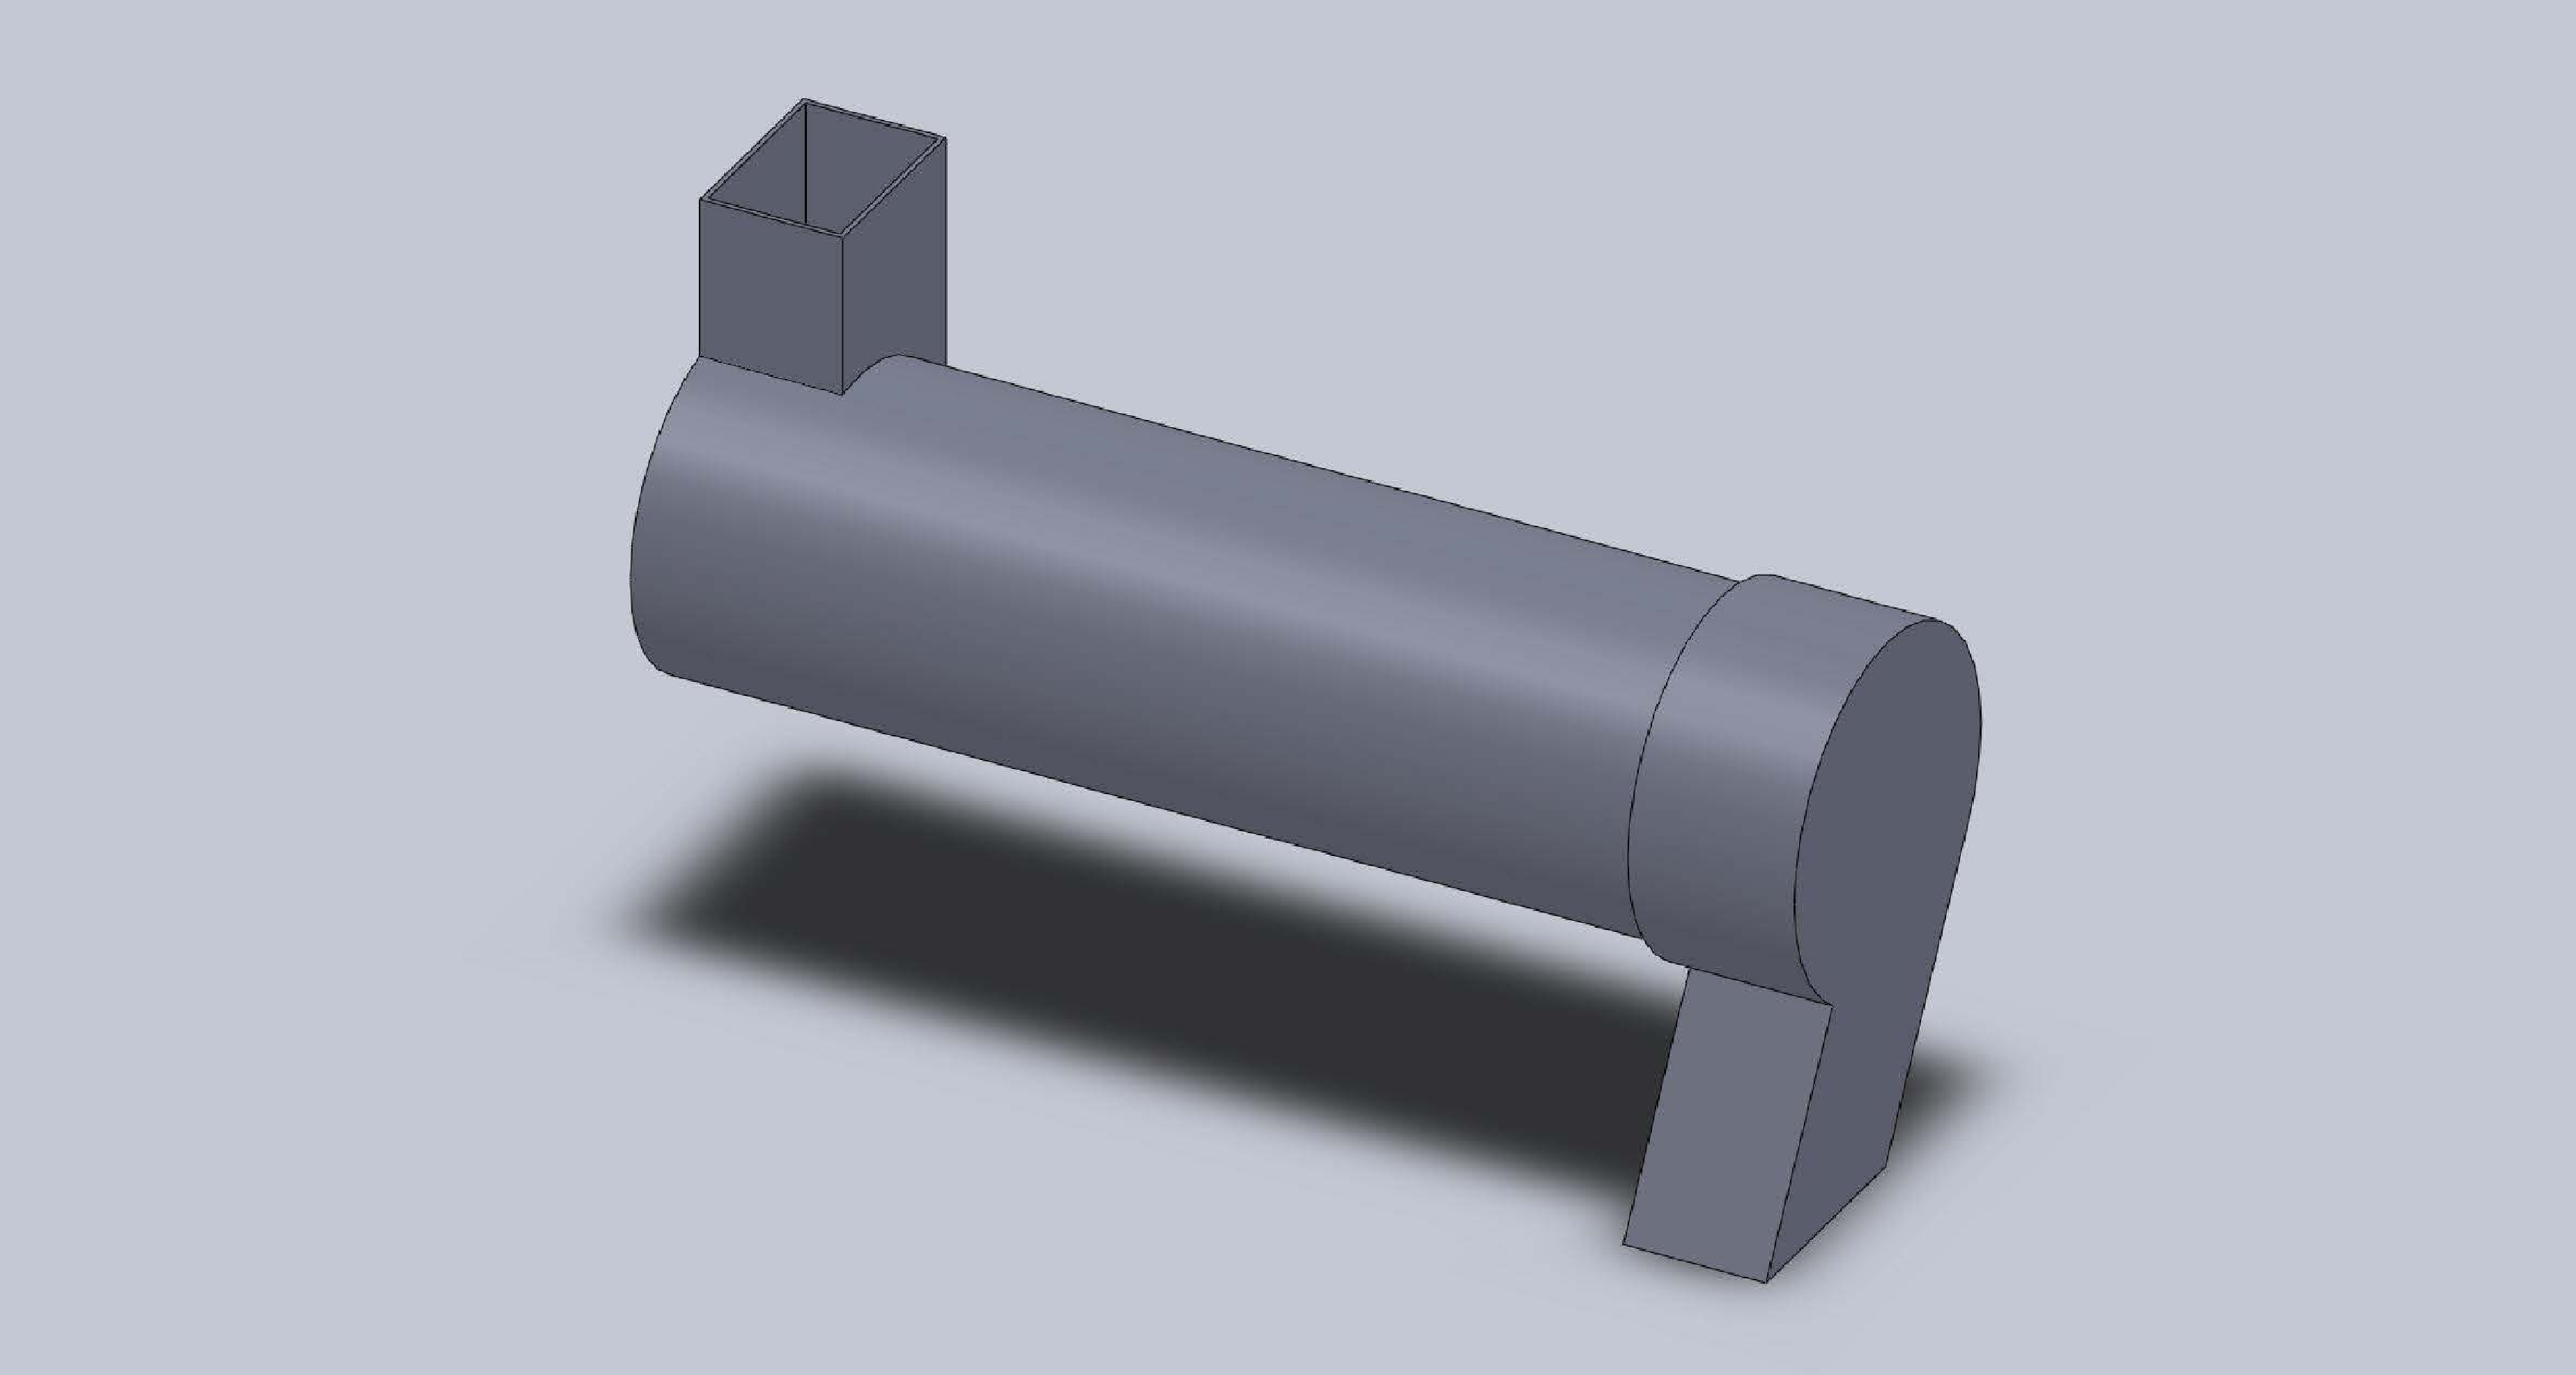
\includegraphics[scale=0.2]{shell_final_pic.pdf}
\caption{The isometric view of the L\"{o}dige CoriMix CM5 continuous high shear granulator casing.}
\label{fig:mthdsDemCharlesGranShell}
\end{figure}

The impeller consists of a cylindrical shaft of length 370 mm and diameter 68 mm with four 
flattened sides 15 mm wide running along the axis. The blades are placed on these flattened sides as 
shown in Figure~\ref{fig:mthds_dem_charles_impeller}. There are three different blade elements on the 
shaft (Figure~\ref{fig:mthds_dem_charles_fig5pt3and4_blades_n_isometric}). At the granulator inlet, 
there are 4 paddle shaped feed elements following which there are 20 tear drop shaped shearing 
elements  and finally 4 trapezoidal blades near the exit. All these elements are placed in 
a spiral configuration. 

\begin{figure}
\centering
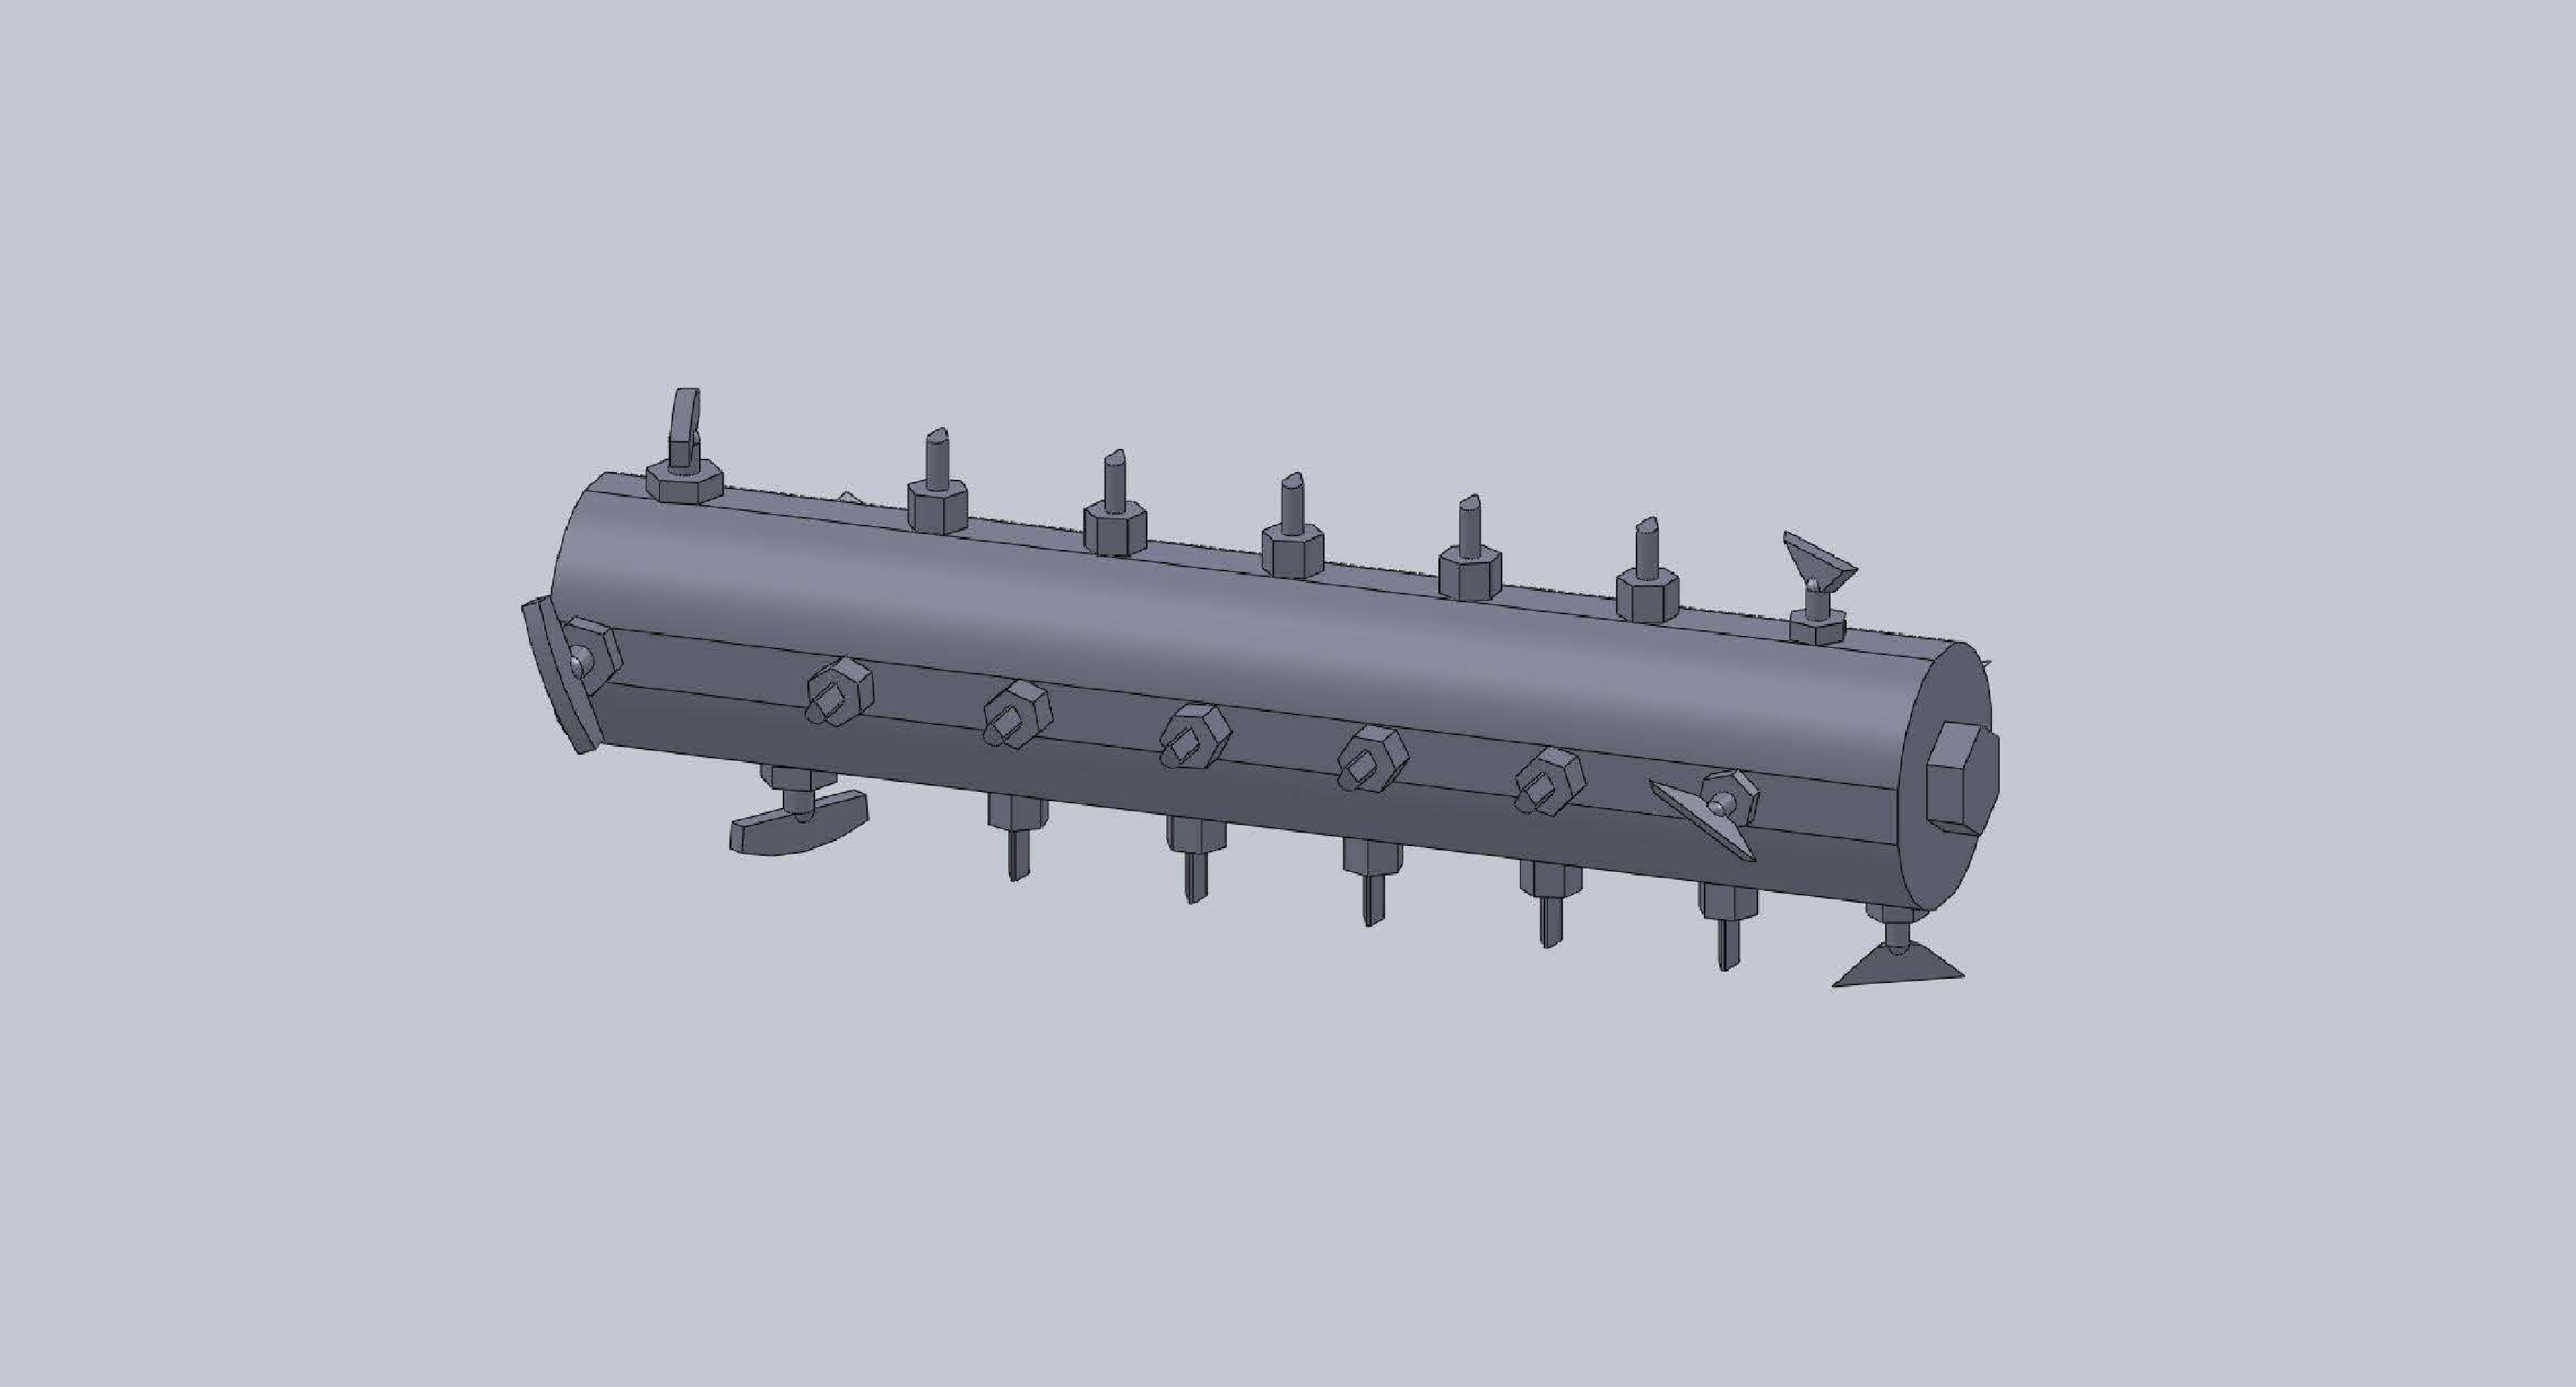
\includegraphics[scale=0.15]{impeller_final_pic.pdf}
\caption{This shows the isometric view of the impeller inside the L\"{o}dige CoriMix CM5 continuous 
high shear granulator casing.}
\label{fig:mthds_dem_charles_impeller}
\end{figure}    

\begin{figure}
\begin{subfigure}{.3\textwidth}
\centering
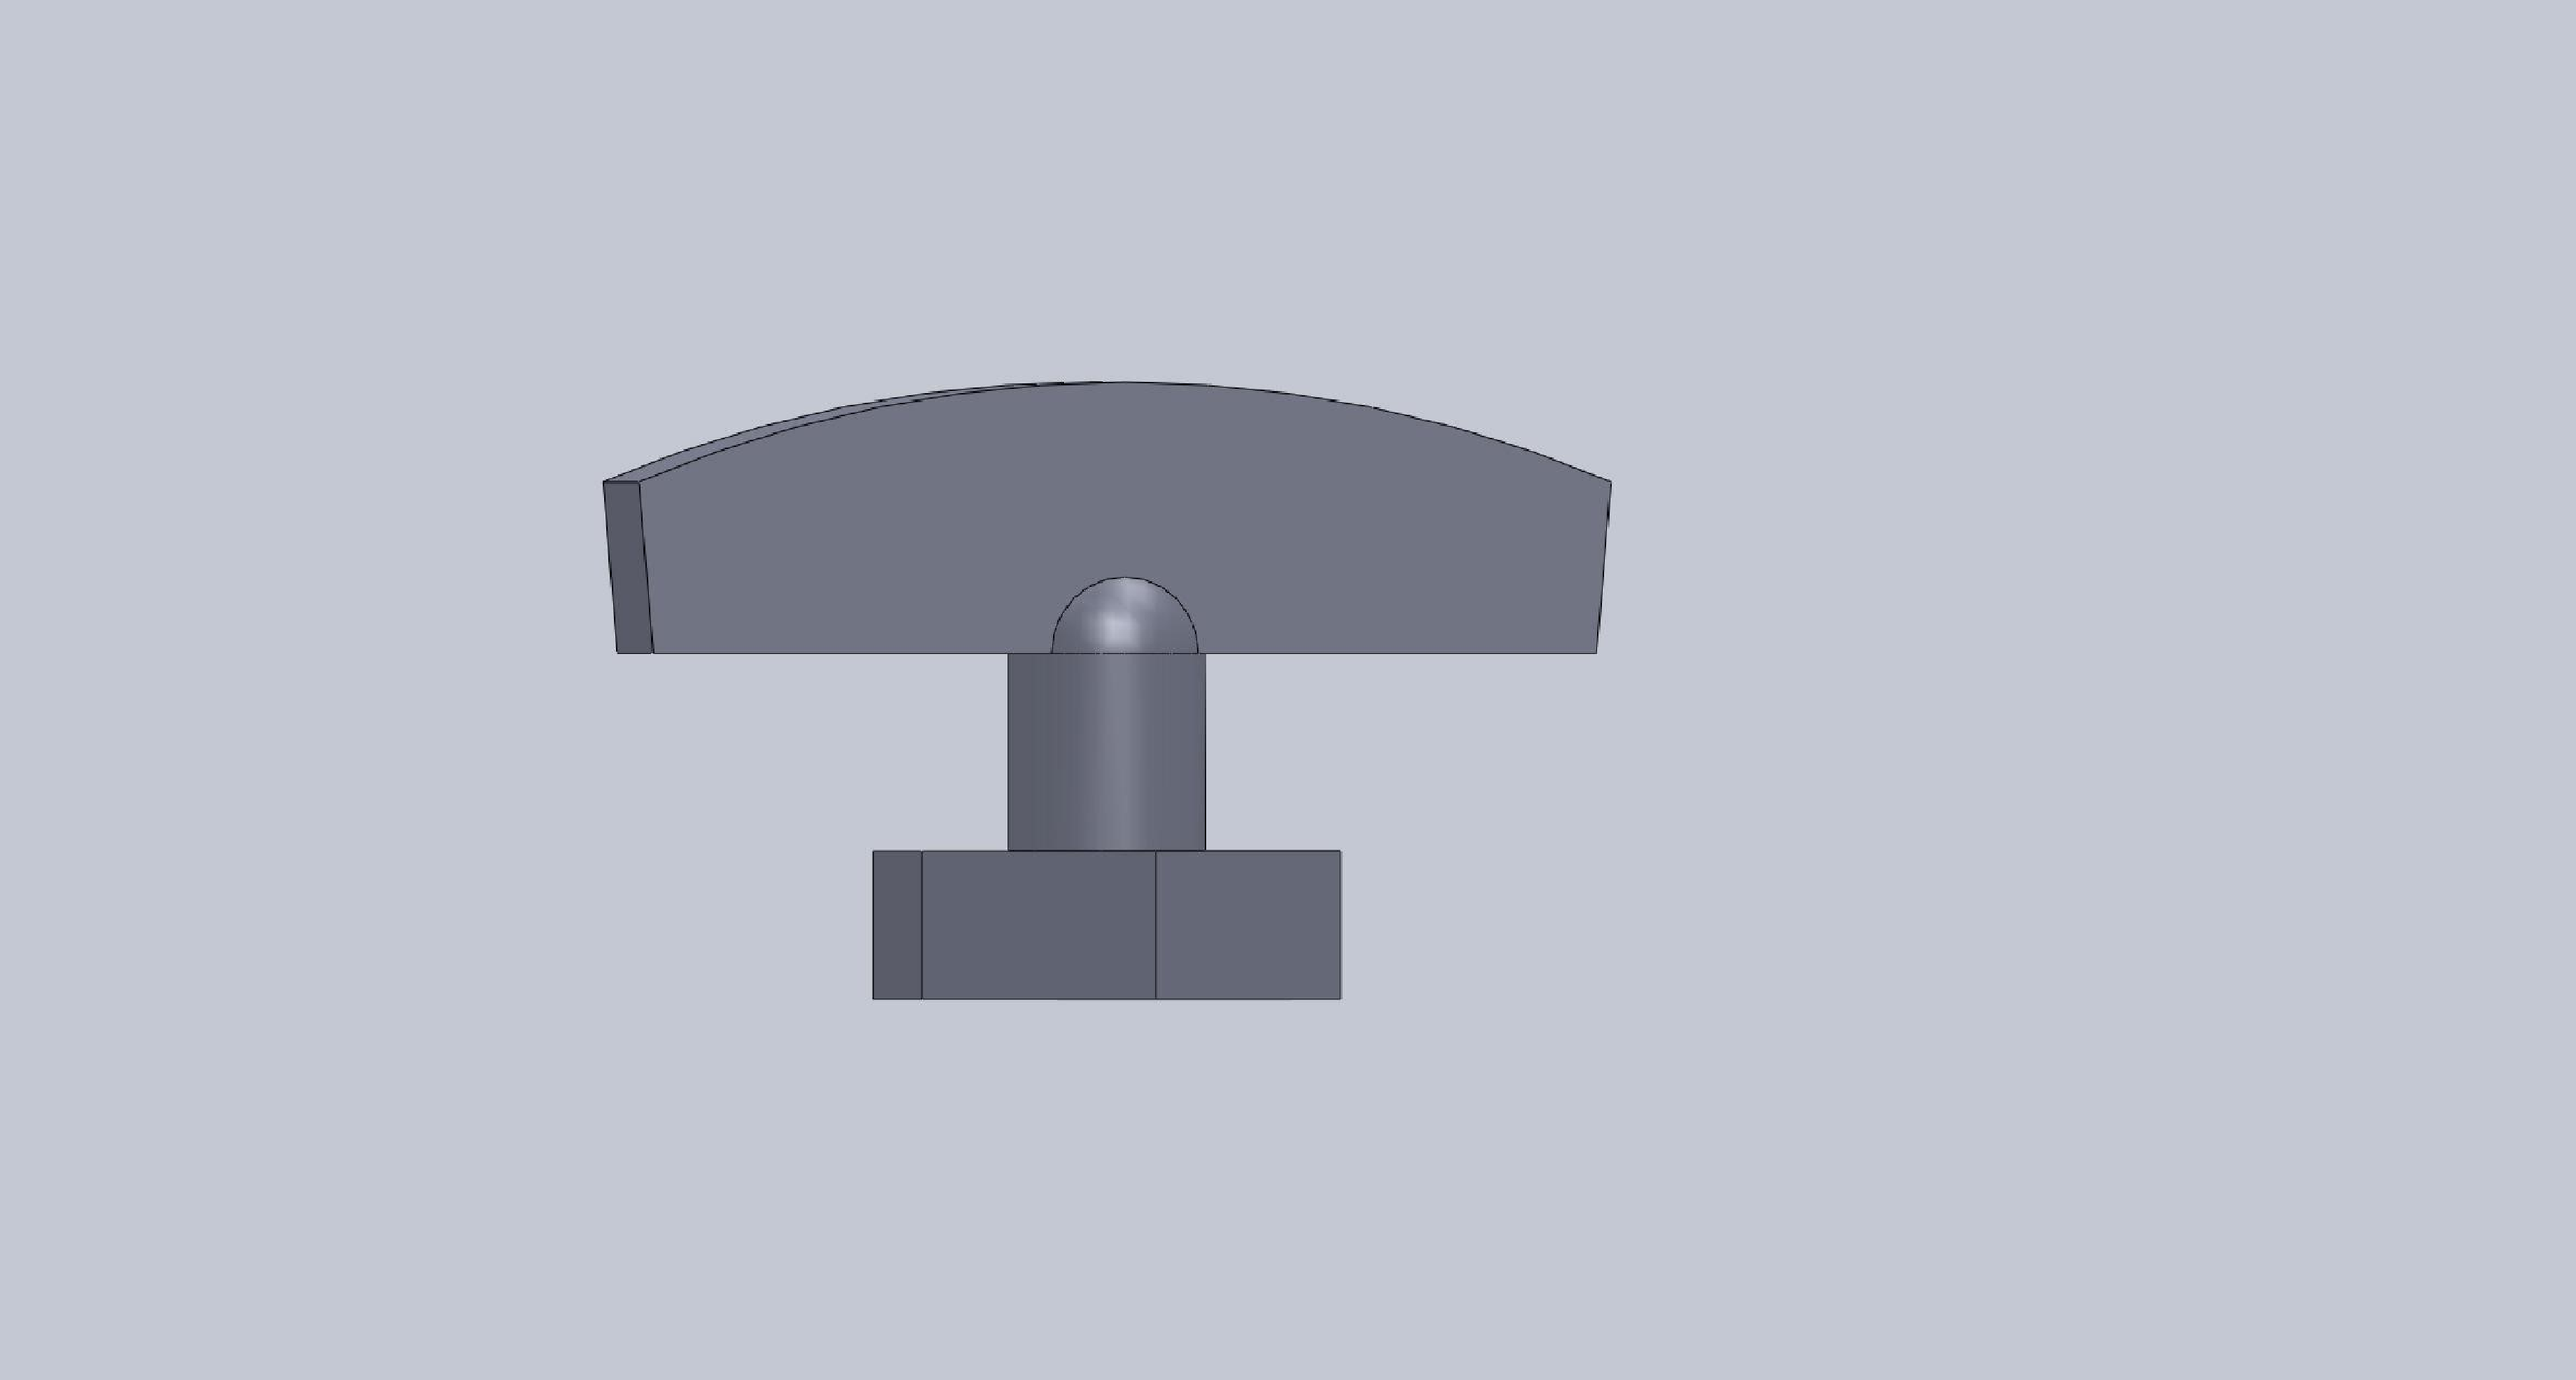
\includegraphics[scale=0.075]{feed_element.pdf}	      
\caption{Feed element}
\label{fig:mthds_dem_feed_element}
\end{subfigure}%
\begin{subfigure}{.3\textwidth}
	\centering
	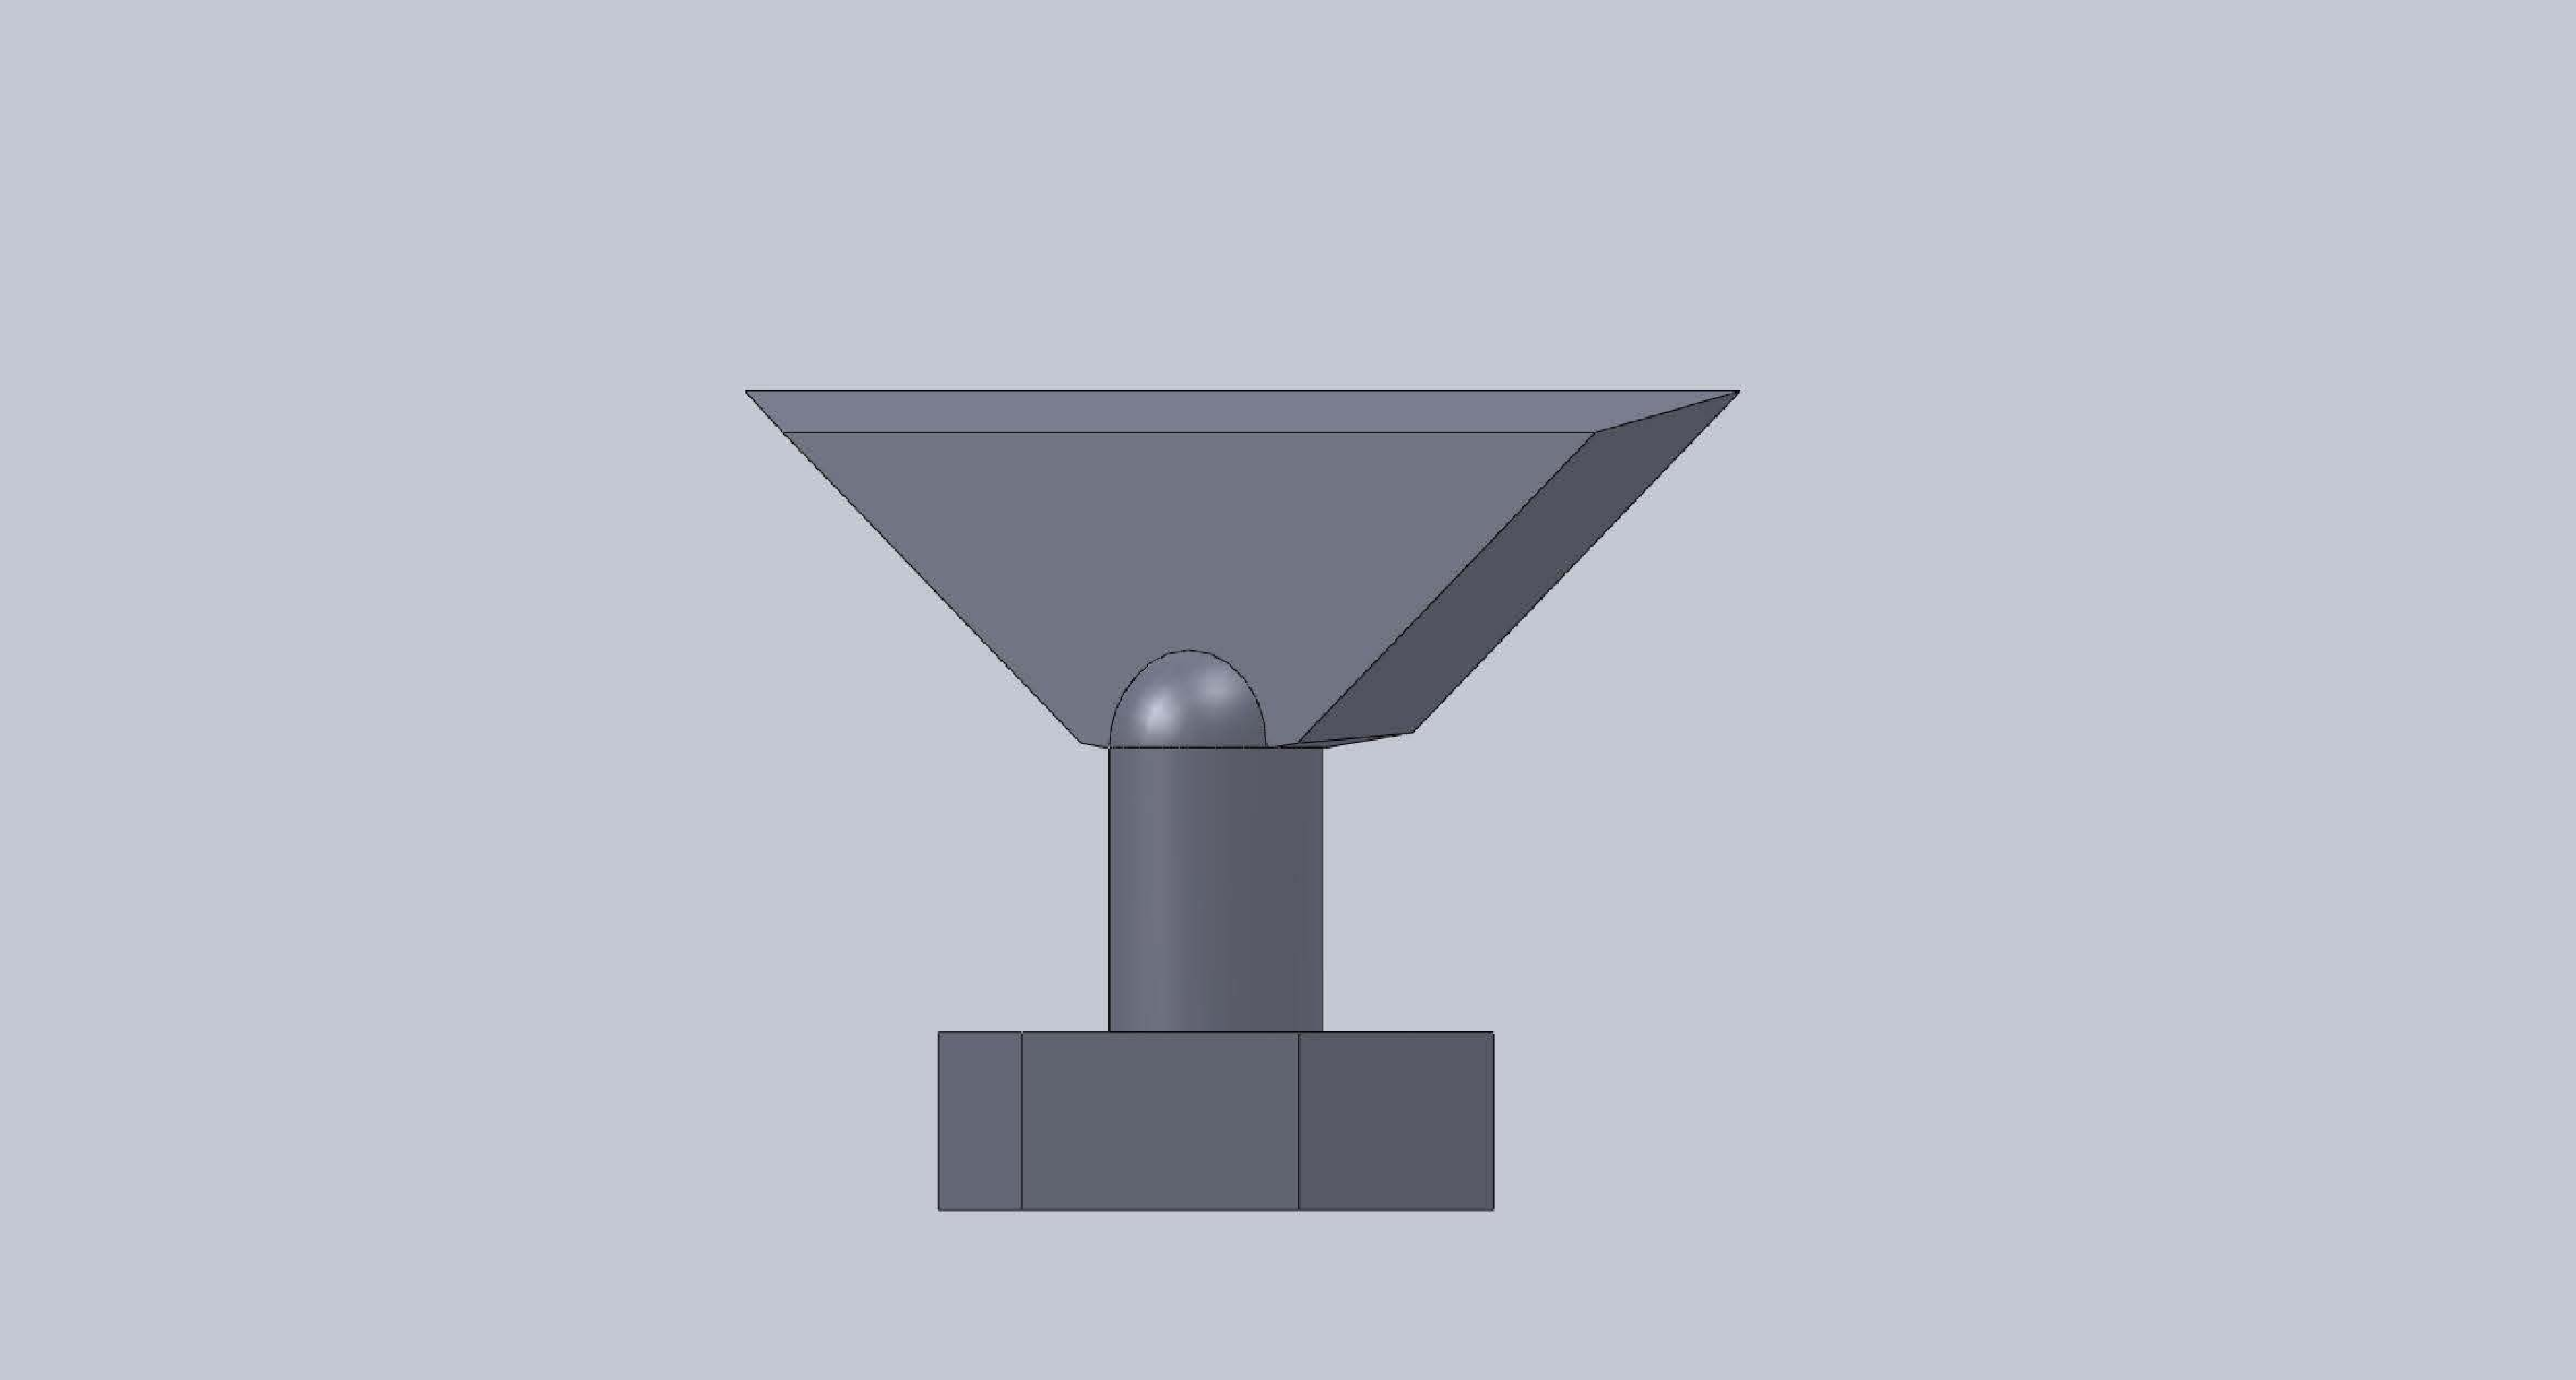
\includegraphics[scale=0.075]{exit_element.pdf}
	\caption{Exit element}
	\label{fig:mthds_dem_exit_element}
\end{subfigure}
\begin{subfigure}{.3\textwidth}
\centering
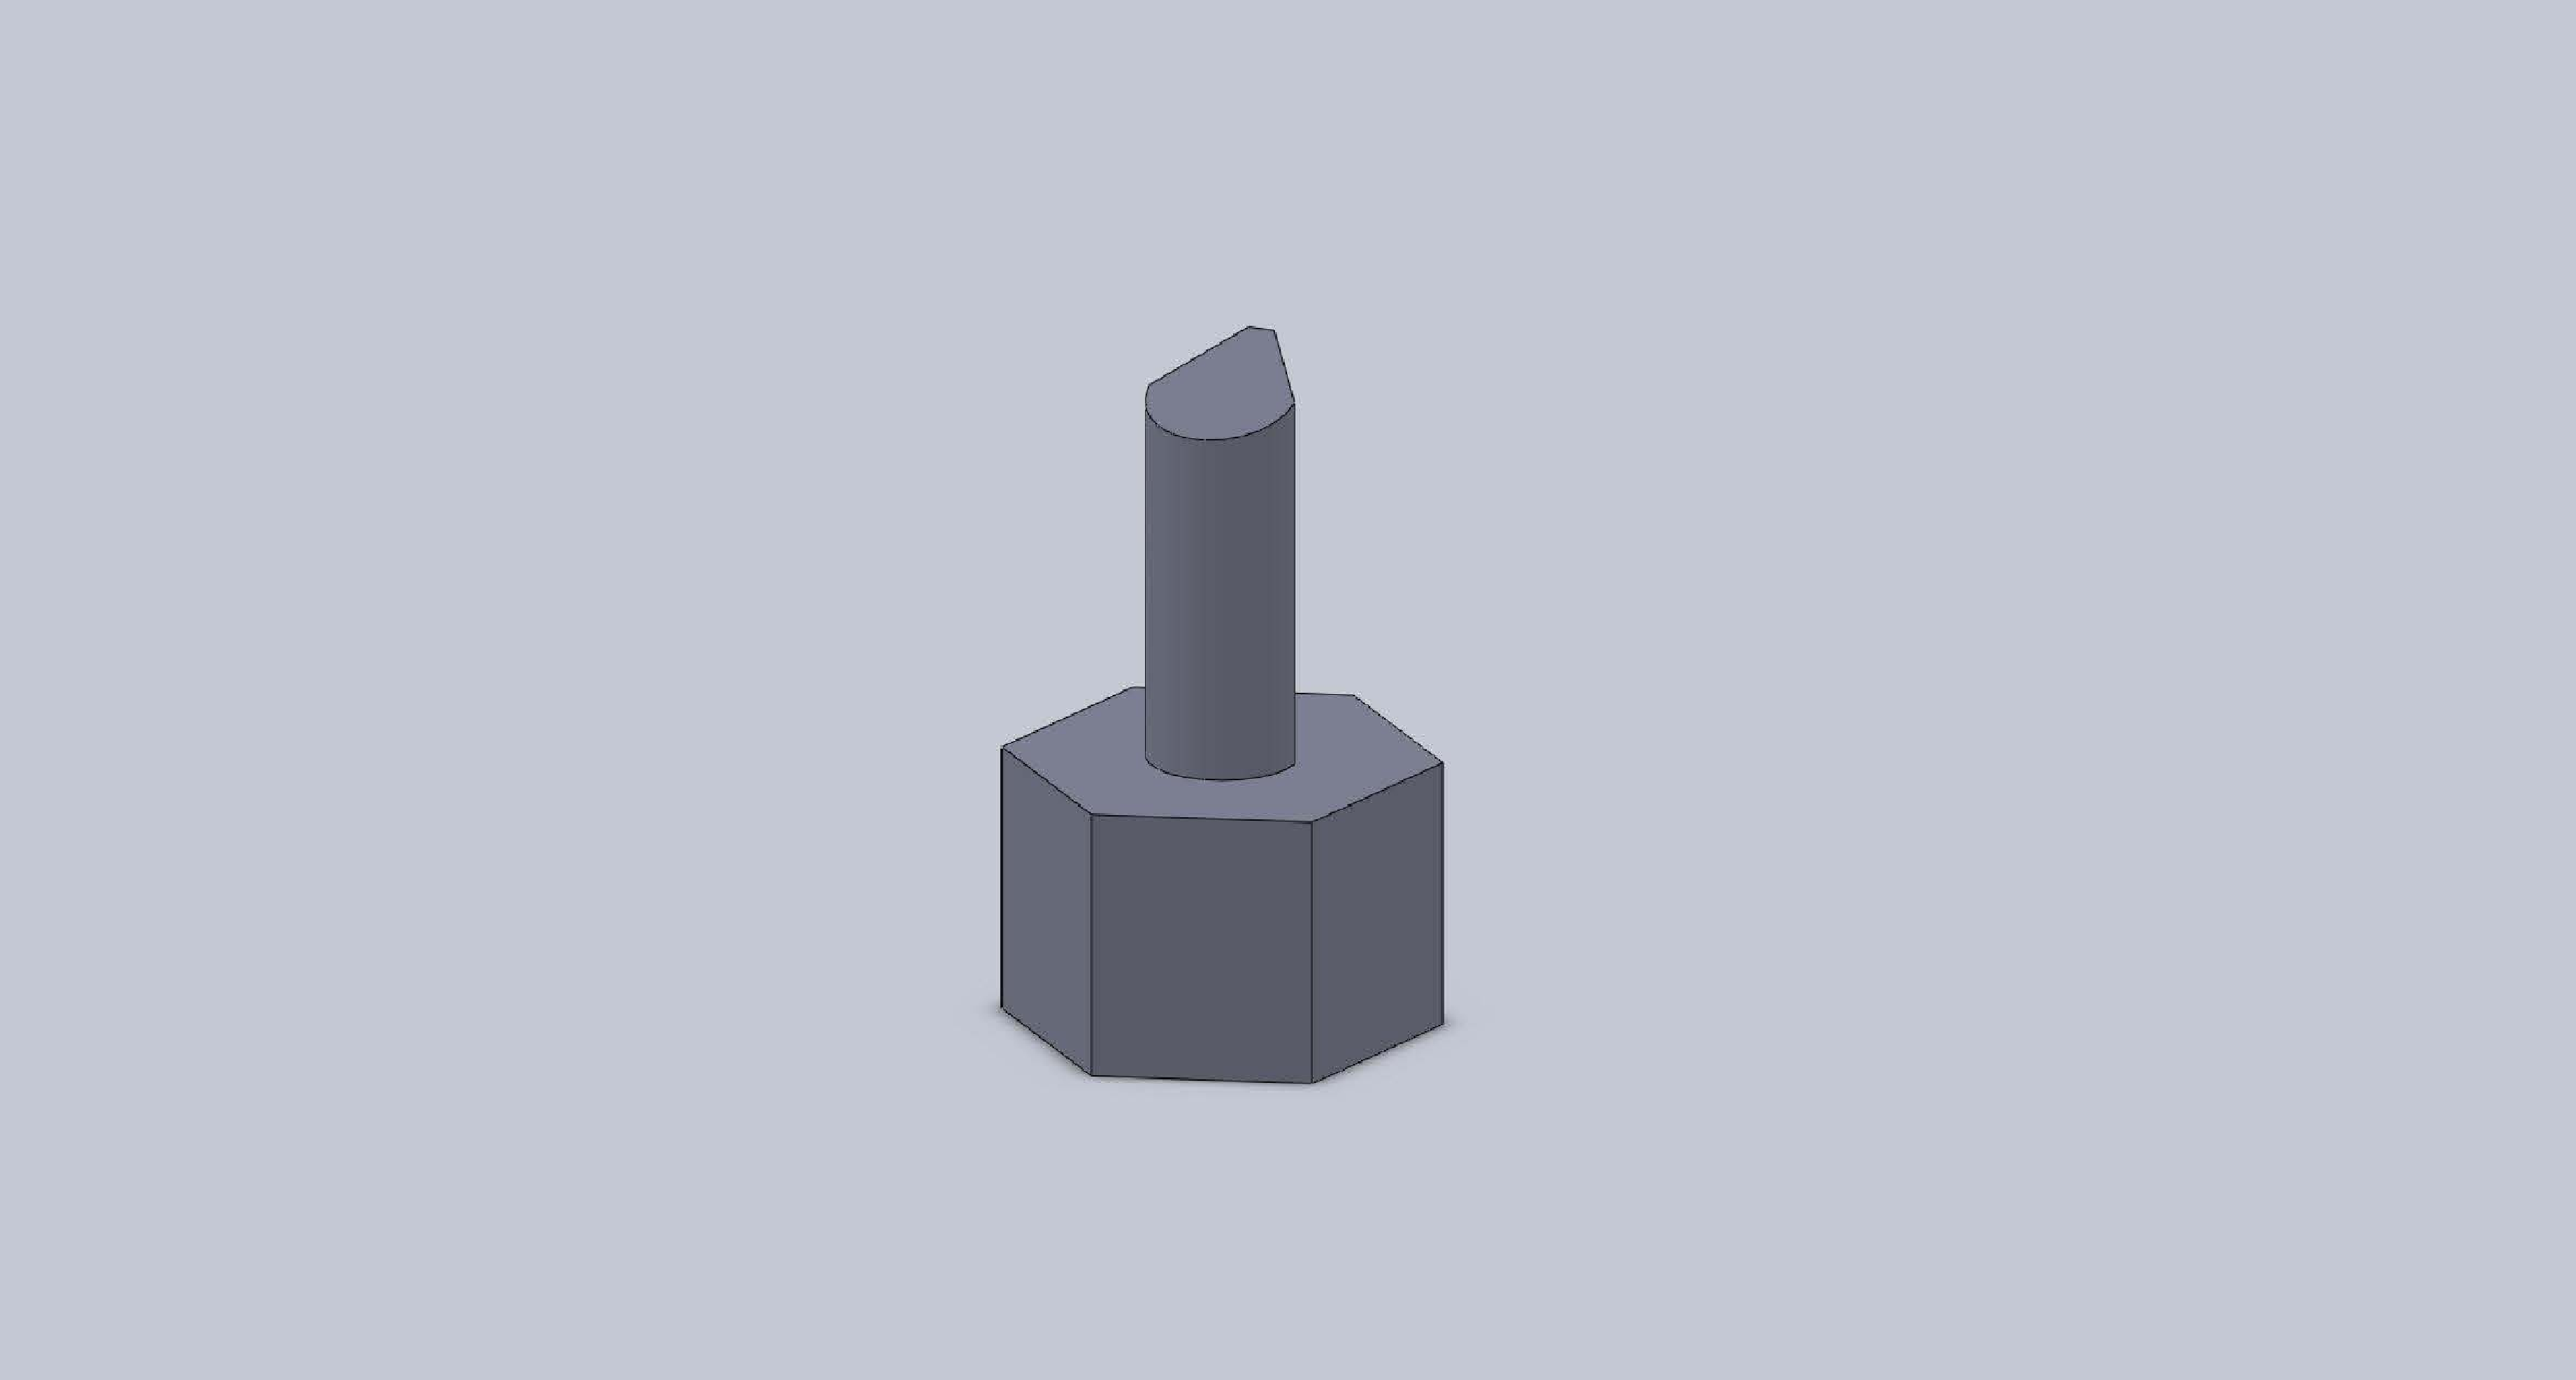
\includegraphics[scale=0.075]{shear_element.pdf}
\caption{Shear element}
\label{fig:mthds_dem_shear_element}
\end{subfigure}
\caption{Components (\subref{fig:mthds_dem_feed_element}) and (\subref{fig:mthds_dem_exit_element}) help in the forward 
movement of the particles while (\subref{fig:mthds_dem_shear_element}) aids to direct the particles to the wall 
inside the L\"{o}dige CoriMix CM5 continuous high shear granulator.}
\label{fig:mthds_dem_charles_fig5pt3and4_blades_n_isometric}
\end{figure}     




\subsubsection{Meshing}
 After the geometry was built in SolidWorks$^{TM}$ (Dassault Syst\`{e}mes) the shell and impeller 
were exported as stereo lithography (STL) files. The coarsest output option was used to keep the STL files 
small and simple for faster computation times. The origin of the geometry was not preserved while saving 
the STL files since it needs to be aligned in LIGGGHTS as per the process conditions.This resulted in 
the impeller having 2802 faces and 1281 points with approximately a file size of 775 kilobytes. 
The shell had 1948 faces and 720 points and size was about 544 kilobytes. Meshlab was used to 
align the STL files for importing into LIGGGHTS. No mesh treatments were used on the STLs. 
The meshes were then imported into LIGGGHTS using the write command in serial. This resulted 
in 50 elements of the impeller file having highly skewed elements, which have more than 5 
neighbors per surface or have an angle less than 0.0181185 radians, that according to LIGGGHTS 
would degrade parallel performance. The write exclusion list command in LIGGGHTS was used and 
this exclusion list file is then used in the simulation to skip the highly skewed elements during 
the simulation. 


\subsubsection{DEM input file settings}
The DEM simulation in LIGGGHTS are setup using an input script which defines the physical 
parameters of the particles, importing of the geometry, particle insertion commands, various physics 
models to be used during the simulation as well as various compute and dump commands to help print 
the data required for post-processing of the data. The particles were considered to be granular in 
nature. The Hertz-Mindlin model was used for non-adhesive elastic contact between the granular particles. 
The particles were inserted inside the granulator from the inlet at a constant mass flow rate of 15 
kilograms per hour. The rotation speed of the impeller was kept throughout the study at 2000 rotations 
per minute. Such a high rotation speed was chosen since this would lead to high shear between the 
particles and the walls of the shell resulting in better size control of the granules. There were 2 sets of 
simulations that were performed, one with mono-sized particles and second consisting of a distribution 
of sizes. The particle radii chosen for mono-sized simulation varied 0.59mm - 2mm, consecutive 
particles radii had volume twice of one before them. The radii range of the distributed size simulation 
was 1mm - 3mm. The difference in the mechanics of these two simulations is discussed in the Section~\ref{sec:Results}. 
The physical constants used for the simulations are given in Table~\ref{table:mthds_dem_input}.

The simulation data was collected after every 50,000 time steps (5$\times 10^{-3}$ sec) 
for the visualization of the particles inside the shell, further post processing . The collisions 
between each of the particles and the collisions between the particle and the geometry was 
collected and used in the PBM. 

\begin{table}
\caption{Physical Properties of the particle for the LIGGGHTS input script} 
\label{table:mthds_dem_input}
\begin{center}
\begin{tabular}{l|c|c}
\hline
\bf{Parameter} &\bf{Value} &\bf{Units}\\
\hline
Young's Modulus of particles  & $8 \times 10^{6}$ & $N.m^{-2}$\\
Young's Modulus of Geometry  & $1 \times 10^{9}$ & $N.m^{-2}$\\
Poisson's Ratio & $0.2$ & $-$\\
Coefficient of restitution (constant for all collisions) & $0.4$ & $-$\\
Coefficient of static friction & $0.5$ & $-$\\
Coefficient of rolling friction  & $0.2$ & $-$\\
Density of the granules & $500$ & $kg.m^{-3}$\\
\hline
\end{tabular}
\end{center}
\end{table}

\subsubsection{DEM data post processing}
The post processing of the data obtained from the DEM simulations was done using MATLAB. 
The first test run on the output data was to determine if the simulation had reached steady-state. The 
mass inside the granulator was found out by averaging it over 5 time steps and then compared to 
mass inside the granulator after every 10000 time steps (about 5$\times 10^{-4}$ sec) with a 
tolerance of about 10\%. If the mass was found to be constant for most of the iterations, it was 
considered to be at steady state. Another test to determine steady state was to monitor the number of 
collision inside the granulator. The visualization of the simulation data was done by running the 
LIGGGHTS post processing (LPP) script over the dump files to convert them into STL files. These 
files were then loaded in to Paraview~\citep{paraview2017} for a graphical 
representation of the 
simulation. It can be seen that the number of collision start to oscillate around a mean value. The 
number of collisions were then plotted and steady state time was determined.
A precautionary script was also run so as to determine that no particles were lost due to overlap 
of the geometry with the particles as well as from particle particle overlap.


\subsection{Population Balance Modeling (PBM)}
\label{sec:pbm_model}
\subsubsection{Model development}
 The population balance equation used in this work is expressed below:
\begin{align}
\frac{d}{dt}F(s_1,s_2,x,t)=\Re_{agg}(s_1,s_2,x,t)+\Re_{break}(s_1,s_2,x,t)+
\dot{F}_{in}(s_1,s_2,x,t)-\dot{F}_{out}(s_1,s_2,x,t)
\label{eqn:mthds_pbm_overall} 
\end{align}
where, $F(s_1,s_2,x)$ is the number of particles with an active pharmaceutical ingredients 
(API) volume of $s_1$ and an excipient 
volume of $s_2$ in the spatial compartment $x$. The rate of change of number of particles with time 
in different size classes depend on the rate of aggregation $\Re_{agg}(s_1,s_2,x)$ and the rate of 
breakage $\Re_{break}(s_1,s_2,x)$. Also, the rate of particles coming into, $\dot{F}_{in}(s_1,s_2,x)$ and 
going out, $\dot{F}_{out}(s_1,s_2,x)$ of the spatial compartment due to particle transfer affect the number of 
particles in different size classes. 
The rate of change of liquid volume for a given time in each particle is calculated using the equation: 

\begin{align}
\frac{d}{dt}F(s_1,s_2,x)l(s_1,s_2,x,t)&= 
\Re_{liq,agg}(s_1,s_2,x)+\Re_{liq,break}(s_1,s_2,x)+\dot{F}_{in}(s_1,s_2,x)l_{in}(s_1,s_2,x)\notag\\
&-\dot{F}_{out}(s_1,s_2,x)l_{out}(s_1,s_2,x)+F(s_1,s_2,x)\dot{l}_{add}(s_1,s_2,x)
\label{eqn:mthds_pbm_rate} 
\end{align}

where, $l(s_1,s_2,x)$ is the amount of liquid volume in each particle with API volume of $s_1$ and 
excipient volume of $s_2$ in the spatial compartment $x$. $\Re_{liq,agg}(s_1,s_2,x)$ and 
$\Re_{liq,break}(s_1,s_2,x)$ are respectively the rates of liquid transferred between size classes due to 
aggregation and breakage. $l_{in}(s_1,s_2,x)$ and $l_{out}(s_1,s_2,x)$ are respectively the liquid 
volumes of the particles coming in and going out of the spatial compartment.~$\dot{l}_{add}(s_1,s_2,x)$ is 
the volume of liquid acquired by each particle in the compartment at every time step due to external 
liquid addition.
Similarly, the rate of change of gas volume for a given time is calculated using the following equation: 

\begin{align}
\frac{d}{dt}F(s_1,s_2,x)g(s_1,s_2,x)&= 
\Re_{gas,agg}(s_1,s_2,x)+\Re_{gas,break}(s_1,s_2,x)+\dot{F}_{in}(s_1,s_2,x)g_{in}(s_1,s_2,x)\notag\\
&-\dot{F}_{out}(s_1,s_2,x)g_{out}(s_1,s_2,x)+F(s_1,s_2,x)\dot{g}_{cons}(s_1,s_2,x)
\label{eqn:mthds_pbm_gas_agg} 
\end{align}

where, $g(s_1,s_2,x)$ is the gas volume of each particle with API volume of $s_1$ and excipient 
volume of $s_2$ in the spatial compartment $x$. $\Re_{gas,agg}(s_1,s_2,x)$ and 
$\Re_{gas,break}(s_1,s_2,x)$ are respectively the rates of gas transferred between size classes due to 
aggregation and breakage. $g_{in}(s_1,s_2,x)$ and $g_{out}(s_1,s_2,x)$ are respectively the gas 
volume of the particles entering and leaving the spatial compartment. $\dot{g}_{cons}(s_1,s_2,x)$ is the 
volume of gas coming out of each particle at every time-step due to consolidation of the particles. 
The rate of aggregation, $\Re_{agg}(s_1,s_2,x)$ in Equation~\ref{eqn:mthds_pbm_overall} is 
calculated as:~\citep{Chaturbedi2017}

\begin{align}
\Re_{agg}(s_1,s_2,x)&= \frac{1}{2}\int _0^{s_1} \int_0^{s_2} 
\beta(s_1',s_2',s_1-s_1',s_2-s_2',x)F(s_1',s_2',x)F(s_1-s_1',s_2-s_2',x)ds_1'ds_2'\notag\\ 
&- F(s_1,s_2,x)\int _0^{s_{max_1}-s_1} \int_0^{s_{max_2}-s_2} 
\beta(s_1,s_2,s_1',s_2',x)F(s_1',s_2',x)ds_1'ds_2'
\end{align}


where, the aggregation kernel, $\beta(s_1,s_2, s_1',s_2',x)$ is expressed as a function of collision 
rate coefficient ($C$) and probability that collision results in agglomeration($\psi$)~\citep{ingram2004}
and is shown below: 

\begin{align}
\beta(s_1,s_2,s_1',s_2',x) = \beta_oC(s_1,s_2,s_1',s_2',x)\psi(s_1,s_2,s_1',s_2',x)
%\beta(s_1,s_2,s_1',s_2',x) = & \beta_o*(V(s_1,s_2,x)+V(s_1',s_2',x))^{\gamma}*(c(s_1,s_2,x)\notag\\
%&+c(s_1',s_2',x))^{\alpha}\left(1-\frac{(c(s_1,s_2,x)+c(s_1',s_2',x))^{\delta}}{2}\right)^{\alpha}
\label{eqn:mthds_pbm_beta_kernal}
\end{align}

where, $\beta_o$ is aggregation rate constant.\\
Collision rate coefficient ($C$) is a function of particle sizes and is calculated by normalizing the 
number of collisions between group of particles~\citep{gantt2006} and is obtained from LIGGGHTS 
DEM simulation. A recent study shows that collision frequency depends on the Particle Size Distribution (PSD) as well~\citep{sen2014}. Collision rate coefficient for every time step can be expressed as:

\begin{align}
C(s_1,s_2,s_1',s_2')=\frac{N_{coll}(s_1,s_2,s_1',s_2')}{N_p(s_1,s_2)N_p(s_1',s_2')\Delta t}
\label{eqn:collfreq}
\end{align}

In Equation~\ref{eqn:collfreq}, $N_{coll}$ is the number of collision between two particles in 
time interval $\Delta t$ \& $N_p$ is number of particle of particular size. The agglomeration 
($\psi$) in Equation~\ref{eqn:mthds_pbm_beta_kernal} can be expressed as:

\begin{align}
\psi((s_1,s_2,s_1',s_2') = 
\left\{\begin{matrix}
\psi_0,\hspace{0.2cm} LC((s_1,s_2) \geq LC_{min}\hspace{0.2cm} and\hspace{0.2cm} LC((s_1',s_2') \geq LC_{min}	\\ 
0,\hspace{0.2cm} LC((s_1,s_2) < LC_{min}\hspace{0.2cm} or\hspace{0.2cm} LC((s_1',s_2') < LC_{min}
\end{matrix}\right.
\label{eqn:colleff}
\end{align}
 In Equation~\ref{eqn:colleff}, $LC$ is the liquid content of particles and $LC_{min}$ stands for minimum 
 liquid content required for coalescence of particles. 

The rate of increase of liquid volume of a particle, $\dot{l}_{add}(s_1,s_2,x)$ is expressed as:

\begin{align}
\dot{l}_{add}(s_1,s_2,x) = \frac{(s_1+s_2)(\dot{m}_{spray}(1-c_{binder})-\dot{m}_{evap})}{m_{solid}(x)}
\end{align}

where, $(s_1+s_2)$  is the total solid volume of the particle; $\dot{m}_spray$ is the rate of external 
liquid addition, $c_{binder}$ is the concentration of binder in the external liquid (which is assumed to 
be zero in this case); $\dot{m}_{evap}$ is the rate of evaporation of liquid from 
the system (which is also assumed to be zero in this case) and $m_{solid}$ is the total amount of solid 
present in the compartment.
The rate of decrease in gas volume per particle due to for a time step consolidation is calculated using the 
following expression:~\citep{Verkoeijen2002} 

\begin{align}
\dot{g}_{cons}(s_1,s_2,x)=&c (\nu_{impeller})^{\omega}V(s_1,s_2,x)\frac{(1-\epsilon_{min})}{s} 
\notag \\ 
& \left[g(s_1,s_2,x)+l(s_1,s_2,x) -(s_1+s_2)\frac{\epsilon_{min}}{1-\epsilon_{min}}\right]
\end{align}        

 where, $c$ and $\omega$ are the consolidation constants; $v_{impeller}$ is the impeller 
rotational speed; $V(s_1,s_2,x)$ is the volume of particle, $\epsilon_{min}$ is the minimum porosity; 
$g(s_1,s_2,x)$ and $l(s_1,s_2,x)$ are respectively the gas and liquid volumes of the particle.

Particle transfer rate, $\dot{F}_{out}(s_1,s_2,x)$ in Equation~\ref{eqn:mthds_pbm_overall} is calculated 
as:

\begin{align}
\dot{F}_{out}(s_1,s_2,x) = \dot{F}(s_1,s_2,x)\frac{\nu_{compartment}(x)*dt}{d_{compartment}}
\end{align}

where, $\nu_{compartment}(x)$ and $d_{compartment}$ are respectively the average velocity of 
particles in compartment $x$ and the distance between the mid-points of two adjacent compartment, 
which is the distance particles have to travel to move to the next spatial compartment. $dt$ is the 
time-step.
The process parameters and physical constants used in the PBM simulation are listed in Table~\ref{table:mthds_pbm_parameters}.
\begin{table}
\caption{Parameters used in the PBM simulation}
\label{table:mthds_pbm_parameters}
\begin{center}
\begin{tabular}{l|c|c|c}
\hline
\bf{Parameter} &\bf{Symbol} &\bf{Value} &\bf{Units}\\
\hline
Initial time step & $\delta t$ & $0.5$ & $s$\\
Mixing time & $T$ & $25$ & $s$\\
Granulation time & $T$ & $75$ & $s$\\
Velocity in axial direction & $v_{axial}$ & $1$ & $ms^{-1}$\\
Velocity in radial direction & $v_{radial}$ & $1$ & $ms^{-1}$\\
Aggregation constant & $\beta_0$ & $1\times10^{-9}$ & $-$\\
Initial particle diameter & $R$ & $150$ & $\mu m$\\
%Breakage kernel constant & $B$ & $0$ & $-$\\
Diameter of impeller & $D$ & $0.114$ & $m$ \\
Impeller rotation speed & $RPM$ & $2000$ & $rpm$\\
Minimum granule porosity & $\epsilon_{min}$ & $0.2$ & $-$\\
Consolidation rate & $C$ & $0$ & $-$\\
Total starting particles in batch & $F_{initial}$ & $1 \times 10^{6}$ & $-$\\
Liquid to solid ratio & $L/S$ & $0.35$ & $-$ \\
Number of Compartments & $c$ & $16$ & $-$ \\
Number of first solid bins & $s$ & $16$ & $-$\\
Number of second solid bins & $ss$ & $16$ & $-$\\
\hline
\end{tabular}
\end{center}
\end{table}


\subsection{Discretization \& parallelizing PBM}

The PBM was discretized by converting each of its coordinates in to discrete
bins. For the spatial coordinates a linear bin spacing was used. For the
internal coordinates, solid, liquid and gas a non-linear discretization was
used~\citep{barrasso2012}. Once the PBM had been discretized, a finite
differences method was used which created a system of ordinary differential
equations (ODEs)~\citep{Barrasso2015cerd}. The numerical integration technique
used to evaluate the system of ODEs was first order Euler integration as it is
commonly used to solve these types of systems and author found an improvement
in  speed while having minimal impact on accuracy~\citep{Barrasso2013}. In
order to avoid numerical instability due to the explicit nature of the Euler
integration, Courant-Friedrichs-Lewis (CFL) condition must be
satisfied~\citep{courant1967}. For our PBM model, time-step was calculated at
each iteration such that, the number of particles leaving a particular bin at
any time is less than the number of particles present at that
time~\citep{Ramachandran2010}. To obtain the most optimal parallel
performance, when solving the PBM, work loads were distributed in a manner
which took into account the shared and distributed memory aspects of the
clusters, the PBM was being run on. To parallelize the model in a way which
could take advantage of shared memory but still effectively run across a
distributed system both MPI and OMP were implemented. One MPI process was used
per CPU core and one OMP thread was used per CPU core,
as~\cite{Bettencourt2017} found it resulted in the best performance. MPI was
used for message passing from one node to another while OMP was used for
calculations on each node that could be efficiently solved using a shared
memory system.

An algorithm in the form of pseudo code is presented below illustrating how
the calculations are distributed and carried out during the simulation. For
each time step, the MPI processes are made responsible for a specific chunk of
the spatial compartments. \jhanote{please use proper format to present an
algorithm. giannis please use format of CCGrid paper, for example} Then each
OMP thread, inside of each MPI process, is allocated to one of the cores of
multi-core CPU the MPI process is bound too. The OMP threads divide up and
compute $\Re_{agg}$. After $\Re_{agg}$ is calculated the MPI processes
calculate the new PSD value for their chunk at that specific time step,
$F_{t,c}$. The slave processes send their $F_{t,c}$ to the master processes
which collects them into the complete $F_{t,all}$. The master process then
broadcasts the $F_{t,all}$ value to all slave processes. This decomposition of
the data into different CPUs and further into various threads is illustrated
in Figure~\ref{fig:mthds_PBM_decompostion}.

\begin{figure}
\centering
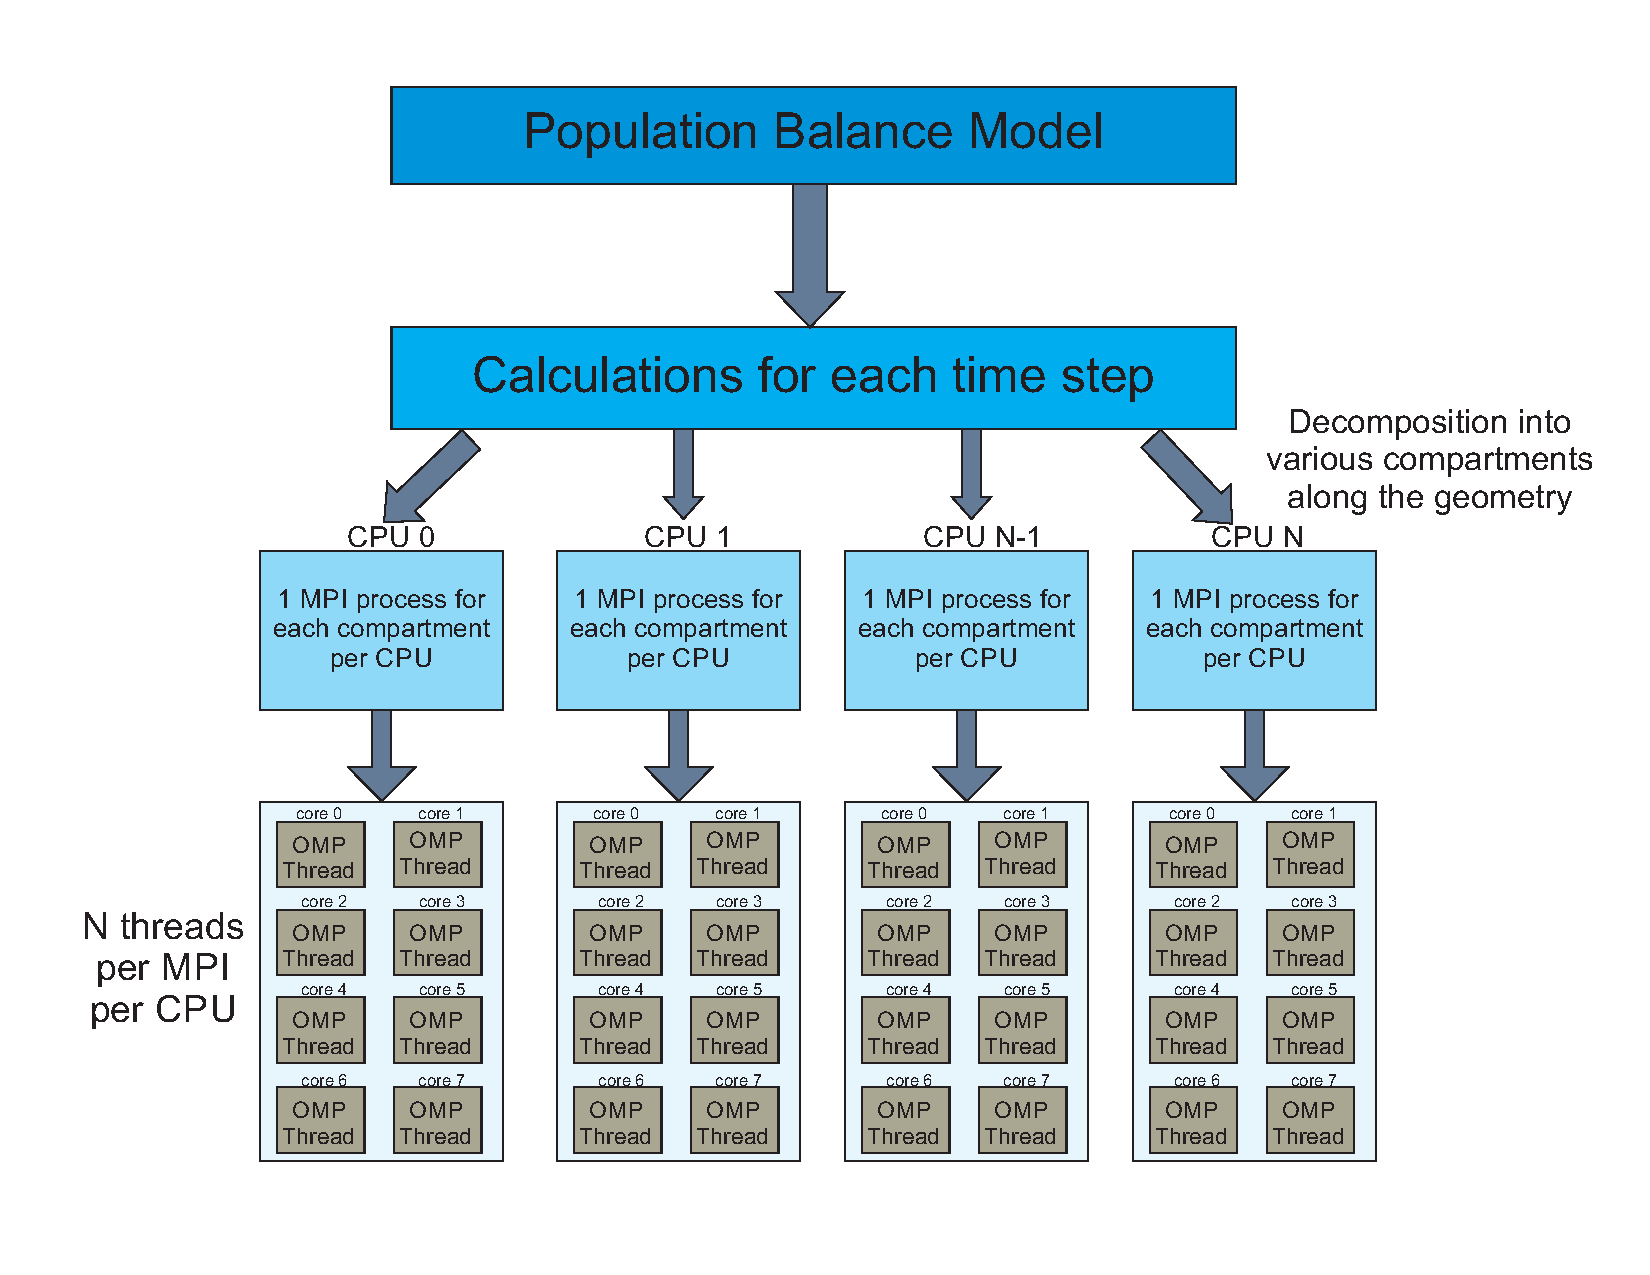
\includegraphics[scale=0.45]{PBM_decomposition.pdf}
\caption{The distribution of the PBM calculations to utilize the MPI + OMP parallelization technique on the CPUs of each node}
\label{fig:mthds_PBM_decompostion}
\end{figure}

A crucial feature of the PBM is that the current PSD ($F_{t,all}$) value is
used to compute a new time step size for the next iteration. This means all of
the MPI processes need to have the same dynamic time step size at each
iteration for the calculations to be properly carried out in parallel. Since
the completely updated $F_{t,all}$ value is shared before calculating a new
time step each process will have the same $F_{t,all}$ value. As a result each
process calculates the same size for the new time step.

Since the DEM informed PBM code required dynamic size increase for the data
structure due to different number of particles being present in the DEM
simulation, the PBM code developed used the Standard Template Library
containers and their features available in \textit{C++} 11 and later. It
requires intel v17.0.2 (gcc 5.3+)  or later for compilation. Since this module
was not present on the Stampede, the execution of the PBM was done on the
newer Stampede2 supercomputer. Each of the compute node of the cluster
consists of Intel Xeon Phi 7250 (\textquotedblleft Knights
Landing\textquotedblright) which has 68 cores on a single socket clocked at
1.4 GHz, with 96 GB of DDR4 RAM. Each of the cores consists of 4 hardware
threads. The simulations were then run by varying the the number of MPI
processes from 1 to 16 and the number of OMP threads from 1 to 8, thus, using
a maximum of 128 cores.

\subsection{Radical Pilot (RP) \& PBM+DEM communication}
\label{sec:RPandCommunications}
RADICAL-Pilot defines a number of abstractions to describe resources, and
computational tasks. The Pilot Description is the abstraction that describes
resources by defining the number of cores that will be used, the used HPC
resource and the total time that the resources are needed, and the queue that
will be used. The abstraction that defines the execution of a computational
task is the Compute Unit (CU). A CU defines the executable, the necessary
environment that is needed during execution, execution arguments, and any file
dependencies the executable may have. RP also defines two managing components,
the Pilot Manager, and Unit Manager. The Pilot Manager is responsible to
submit a Pilot to the selected resources. The Unit Manager is responsible to
place CUs to active Pilots. As soon as a unit is placed in a pilot it starts
executing on the acquired resources.

RADICAL-Pilot was utilized to execute and monitor DEM and PBM simulations.
Initially, a pilot description is created to use several cores of a resource
and submitted to the pilot manager. A CU description is created for the DEM
simulation and submitted to the Unit Manager. As soon as the pilot is active
the DEM simulation start executing. When finished a CU that describes a PBM
simulation is submitted at the Unit Manager and start executing. Any data
dependency is satisfied by doing the necessary file linking through the CU
description.

The DEM and PBM executables are pre-placed in the resource along with any
initial information for the DEM simulation. The DEM unit first creates links
for the data files that will be needed for the DEM simulation and call the
executable. When the execution finishes, new links with the output are created
in a shared space. The PBM unit uses those links to read the necessary data to
execute the simulation. When both have finished RP downloads the PBM results.



\section{Results \& Discussion}
\label{sec:Results}
\subsection{Discrete Element Modeling (DEM)}
\subsubsection{DEM Spatial Decomposition Studies}
LIGGGHTS as discussed previously, statically decomposes the work space and
each section is sent to a MPI process for calculations. Thus, the division of
the space becomes an important criteria for the simulation for efficient load
balancing. The initial studies were undertaken for a mono-sized particle of
size 1 mm and the simulation was carried out for 0.5 second of granulation
time. The initial timing studies for the decomposition were performed using 64
cores. The effect of the decomposition on the simulation time can be seen in
Table~\ref{table:rslts_dem_slicing_studies}. The time values indicate that dividing the
x-direction in more number of compartments decreases the speed of the
simulation. \jhanote{increasing the "speed of the simulation" is typically
associated with improved performance. what you mean here is the converse,
greater the number of compartments, slower the simulation? please clarify or
fix.} \csnote{A good spot! I meant the converse. Have fixed the 2 following lines as well} 
The extra slicing in the x-direction leads to lesser amount of computation required 
for a single process but it also leads to each particle being transferred to 
a new process in lesser number of time steps. Thus, leading to slower simulations when
the number of slices increase beyond 16 in the x-direction. 
%This is easy to comprehend since the granulator has its length parallel to the x-axis. 
Table \ref{table:rslts_dem_slicing_studies} also indicate that if the geometry is divided into
more than 2 compartments in either the y-axis or the z-axis the simulation time
increases. \jhanote{this is inconsistent with results in table 3!} 
This can be accounted to the increased communication required to transfer 
the rotating impeller mesh from one compartment in the y-axis or the z-axis 
to the another compartment for each time step. Since MPI has to pass explicit 
messages in between the nodes for it to communicate data, there is a delay 
associated with the master process to obtain all the data. The master process
need to wait for all the other processes to complete their task before it receives 
the data from all the processes. With the increased 
partitions in the y and the z-axes, the master process needs to wait for more 
processes, leading to delays before the next time step can be simulated which 
in turn makes the simulation slower.\jhanote{this sentence does 
not make sense. MPI is "not limited": it is the message passing interface. 
please rewrite and make consistent with data in table 3, or clarify} 
\csnote{have explained the communications in a better manner} Following the 
results from the initial timing studies,the y and the z-axes were not divided
in more than 2 compartments for 128 and 256 core simulation as well. This
meant that the x-axis was divided into 32 and 64 compartments respectively. 

\begin{table}
\caption{The effect of spatial decomposition on the performance of the DEM simulations using 64 cores.}
\label{table:rslts_dem_slicing_studies}
\begin{center}
\begin{tabulary}{\linewidth}{C|C|C|C}
  
\hline
\bf{Slices in x-direction}&\bf{Slices in y-direction}&\bf{Slices in z-direction}& \bf{Time taken for a 0.5 
second simulation (in minutes)}\\
\hline
$64$ & $1$ & $1$ & $10.27$\\
$32$ & $2$ & $1$ & $8.70$\\
$16$ & $2$ & $2$ & $6.83$\\
$8$ & $4$ & $2$ & $7.20$\\		  
$8$ & $2$ & $4$ & $7.96$\\
\hline  		  
\end{tabulary}
\end{center}
      
\end{table}

%When MPI is used for parallelization of a task, load balancing becomes an
%important parameter that needs to be considered. When the geometry is divided,
%the amount of computation done by one core should be similar to other
%processors. 
\jhanote{What evidence/indication is there that load balancing is
a problem, as opposed to communication limited?} \csnote{The first few lines 
are  just general statments I could do away with this paragraph altogether. 
It does not fit with the flow} %This helps better utilization
%of the resources as well as make the simulations run faster. 
%Following the results from the initial timing studies,the y and the z-axes were not divided
%in more than 2 compartments for 128 and 256 core simulation as well. This
%meant that the x-axis was divided into 32 and 64 compartments respectively. 
\jhanote{1 paragraph, 1 idea. Is the following part of the above 'load balancing' or is 
now about 'communication'?} \csnote{tried to clear the air by removing the general statements}
In order to avoid the expensive communication
between the processes, LIGGGHTS tries to insert the particles towards the
center of the compartment such that the number of ghost atoms are minimized.
For simulations with higher number of cores the extra slicing in the x direction 
reduced the space available for the insertion of the particles.
This made LIGGGHTS carry out larger number of Monte-Carlo simulations to insert 
the partilces in the desired area. In some cases, the Monte-Carlo iterations performed 
were not enought leading to many of the particles being inserted incorrectly.
\jhanote{please elaborate} Another abnormal behavior observed due to this over slicing 
was that the particles halted \jhanote{in a?} in a certain compartment and
no particle traveled beyond this compartment in the x-direction. Thus, the number of partitions 
in the x-direction were reduced and a new set of experiments with different 3-d partition 
configuration were carried out. 
\jhanote{I'm
confused: the previous sentences imply a functional problem. The next sentence
suggests a performance solution. Doesn't make sense to me.}  The
comparison of the simulation times of experiments with the new configurations are shown in
Table~\ref{table:rslts_dem_128_256_decomp}.

\begin{table}
\caption{Comparison of time taken for the DEM simulations using 128 and 256 core due to different spatial decomposition 
configurations.}
\label{table:rslts_dem_128_256_decomp}
\begin{center}
\begin{tabulary}{\linewidth}{C|C|C|C|C}
  
\hline
\bf{Number of cores used}&\bf{Slices in x-direction}&\bf{Slices in y-direction}&\bf{Slices in 
z-direction}& \bf{Time taken for a 10 second simulation (in minutes)}\\
\hline
$128$ & $16$ & $2$ & $4$ & $264.67$\\
$128$ & $16$ & $4$ & $2$ & $247.2$\\
$256$ & $16$ & $2$ & $8$ & $271.5$\\		  
$256$ & $16$ & $8$ & $2$ & $252$\\
$256$ & $16$ & $4$ & $4$ & $265.32$\\
\hline  		  
\end{tabulary}
\end{center}
      
\end{table}
The simulation times illustrated in Table~\ref{table:rslts_dem_128_256_decomp}
show that incorrectly slicing the geometry also affects the performance of the
system. It can be noted that slicing along y-axis is more favorable than
slicing along the z-direction. \jhanote{Without further
discussion/explaination, it is difficult to discern how/why?.} \csnote{Proceeding lines 
have this discussion} The
insertion of particles is hindered when the geometry is cut along the z-axis
as the inlet is perpendicular to it. LIGGGHTS thus provisions less space for
the insertion of these particles, thus increasing the time of the simulation.
Thus, just slicing the geometry into 2 sections along the z-axis is preferred.
So, the chosen configurations for the final simulations consisted of the
geometry having only 2 sections in the z-direction and more slices along the
y-axis.

\subsubsection{DEM Performance}
A test case was run for mono-sized particle of 2mm diameter for timing
comparison studies. The times are plotted in
Figure~\ref{fig:rslts_DEM_2mm_timing} indicate that using lower number of
cores is not feasible for long simulations since the time taken while using 1
core is about $11$x times slower. Thus, the simulations were carried out in
core configurations of 64, 128 and 256 cores. The studies undertaken had 5
mono-sized population of particles of diameter 0.63, 1, 1.26, 1.59 and 2 mm
simulations and one simulation consisted of particle size distribution.
Figure~\ref{fig:rslts_DEM_timing_studies} shows that the amount of CPU time
required for a 10 second simulation of the granulator. The post processing
MATLAB script was run on the dump files obtained from the simulation and it
was observed that the system reached a steady state about 3-5 seconds of the
simulation time. Particles with larger diameter reached steady state at a
faster rate with an average hold-up of particles of about 6500.
\begin{figure}
\centering
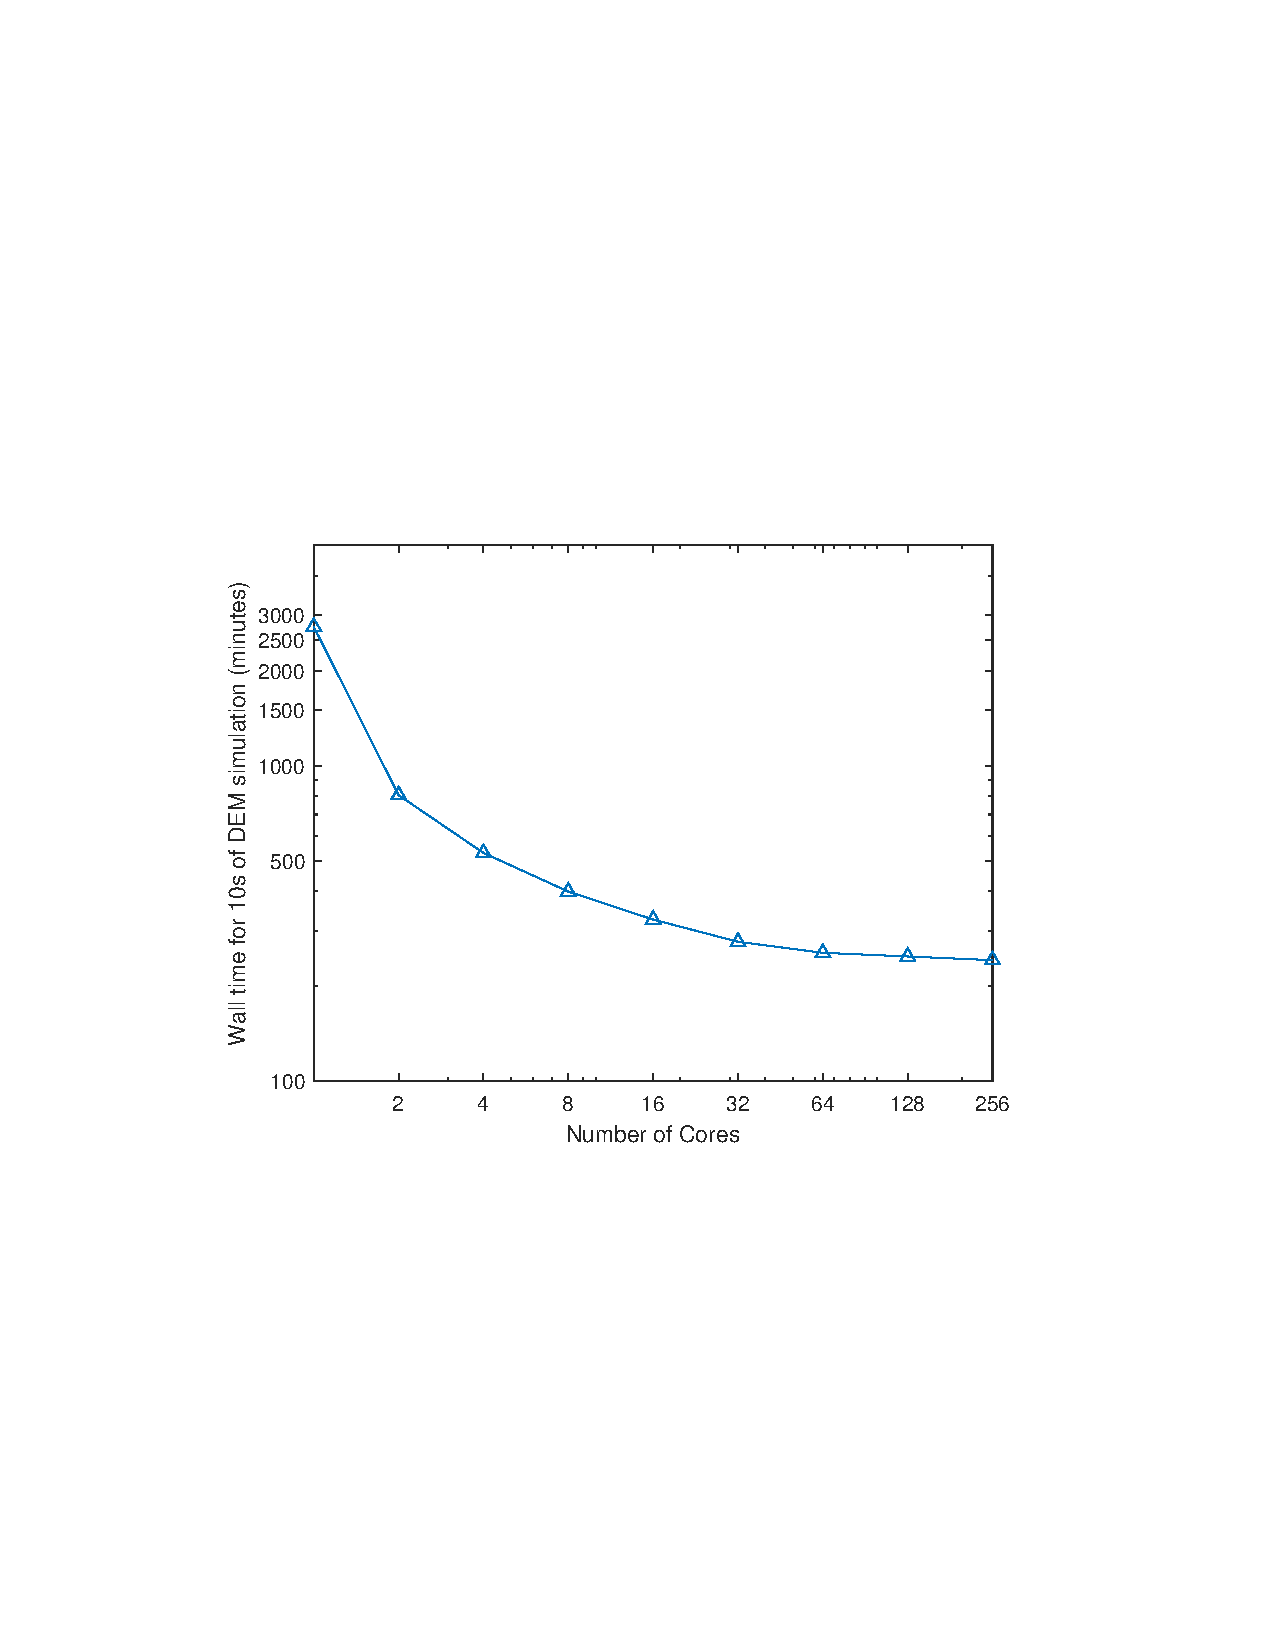
\includegraphics[scale=0.75]{rslsts_2mm_timing_mtlb.pdf}
\caption{The variation in the amount of time taken for the DEM simulation of 2 mm particles as a function of number of cores. 
The improvements in the speed of the simulation was higher when the cores were increased from 1 
16 when compared to speed improvements obtained with a core count greater than 16.}
\label{fig:rslts_DEM_2mm_timing}
\end{figure}	

Pure timing studies are not really a good measure to represent the parallel performance of a program. 
Speedup of a parallel program indicates the speed increase of the program when it is run on more 
compute cores compared to the wall clock time when it is run in serial. It is the most common way to 
represent the parallel performance. Speedup is the ratio of the time taken to run the program in serial 
to the time taken by the program to run in parallel as shown in Equation~\ref{eqn:rslts_DEM_Speed_Up}. 
For an ideally parallelized program, the speedup is 'n' times, where n is the number of cores used.

\begin{align}
\textit{Speedup} = \frac{\textit{Serial Wall Clock Time}}{\textit{Parallel Wall Clock Time}}
\label{eqn:rslts_DEM_Speed_Up}
\end{align}

Speedup does not take into account number of processors used in the simulation, thus another metric 
that is used to determine the parallel performance is parallel efficiency. This metric is nothing by 
speedup divided by the number of cores used. Thus, parallel efficiency normalizes speedup and gives 
a fractional value of the ideal speedup a program achieves with the increase in the number of cores.

\begin{align}
\textit{Parallel Efficiency} = \frac{\textit{Serial Wall Clock Time}}{\textit{Parallel Wall Clock Time $\times$ $n_{cores}$}}
\label{eqn:rslts_DEM_parallel_efficiency}
\end{align}

The speedup of the DEM simulations using only MPI cores is shown in Figure~\ref{fig:rslts_DEM_speedup}.
There is a linear speed increase in the speedup up to 16 cores, after which the 
performance plateaus.
Figure~\ref{fig:rslts_DEM_speedup} indicates that there 
is not a significant amount of speed improvement for the simulation when 256 cores are used for the 
simulation over 128 cores. This speed decrease can be accounted to the communication time between 
the MPI processes. When the particles move from one section to another of the space, they are 
transferred as ghost particles from one process to another process. Thus, there is large amount of 
communication which is required. One of the issues of using a cluster with shared memory within 
the nodes but none in between nodes is that it has to rely on the networking infrastructure 
of the cluster which bottlenecks the communications thus leading to higher communication times. 
There are more sections present when 256 cores are used for the simulation, thus there is more 
communication in this system when compared to 128 core simulation. 
This excess communication makes the simulation slower though there is more processing power and 
it requires lesser time for other calculations. Another observation that can be made from Figure~\ref{fig:rslts_DEM_timing_studies} is that the particle size distribution simulation takes more time 
compared to the simulations with mono-sized particles of 1.59mm and 2mm, though the mean size of 
particles in the distribution is 2mm. The default profile provided by LIGGGHTS indicates that the time 
spent in calculating the particle-particle interaction forces was higher than the mono-sized 
simulations. The different diameters make the interaction forces more tedious thus, making it 
computationally more expensive. 

\begin{figure}
\centering
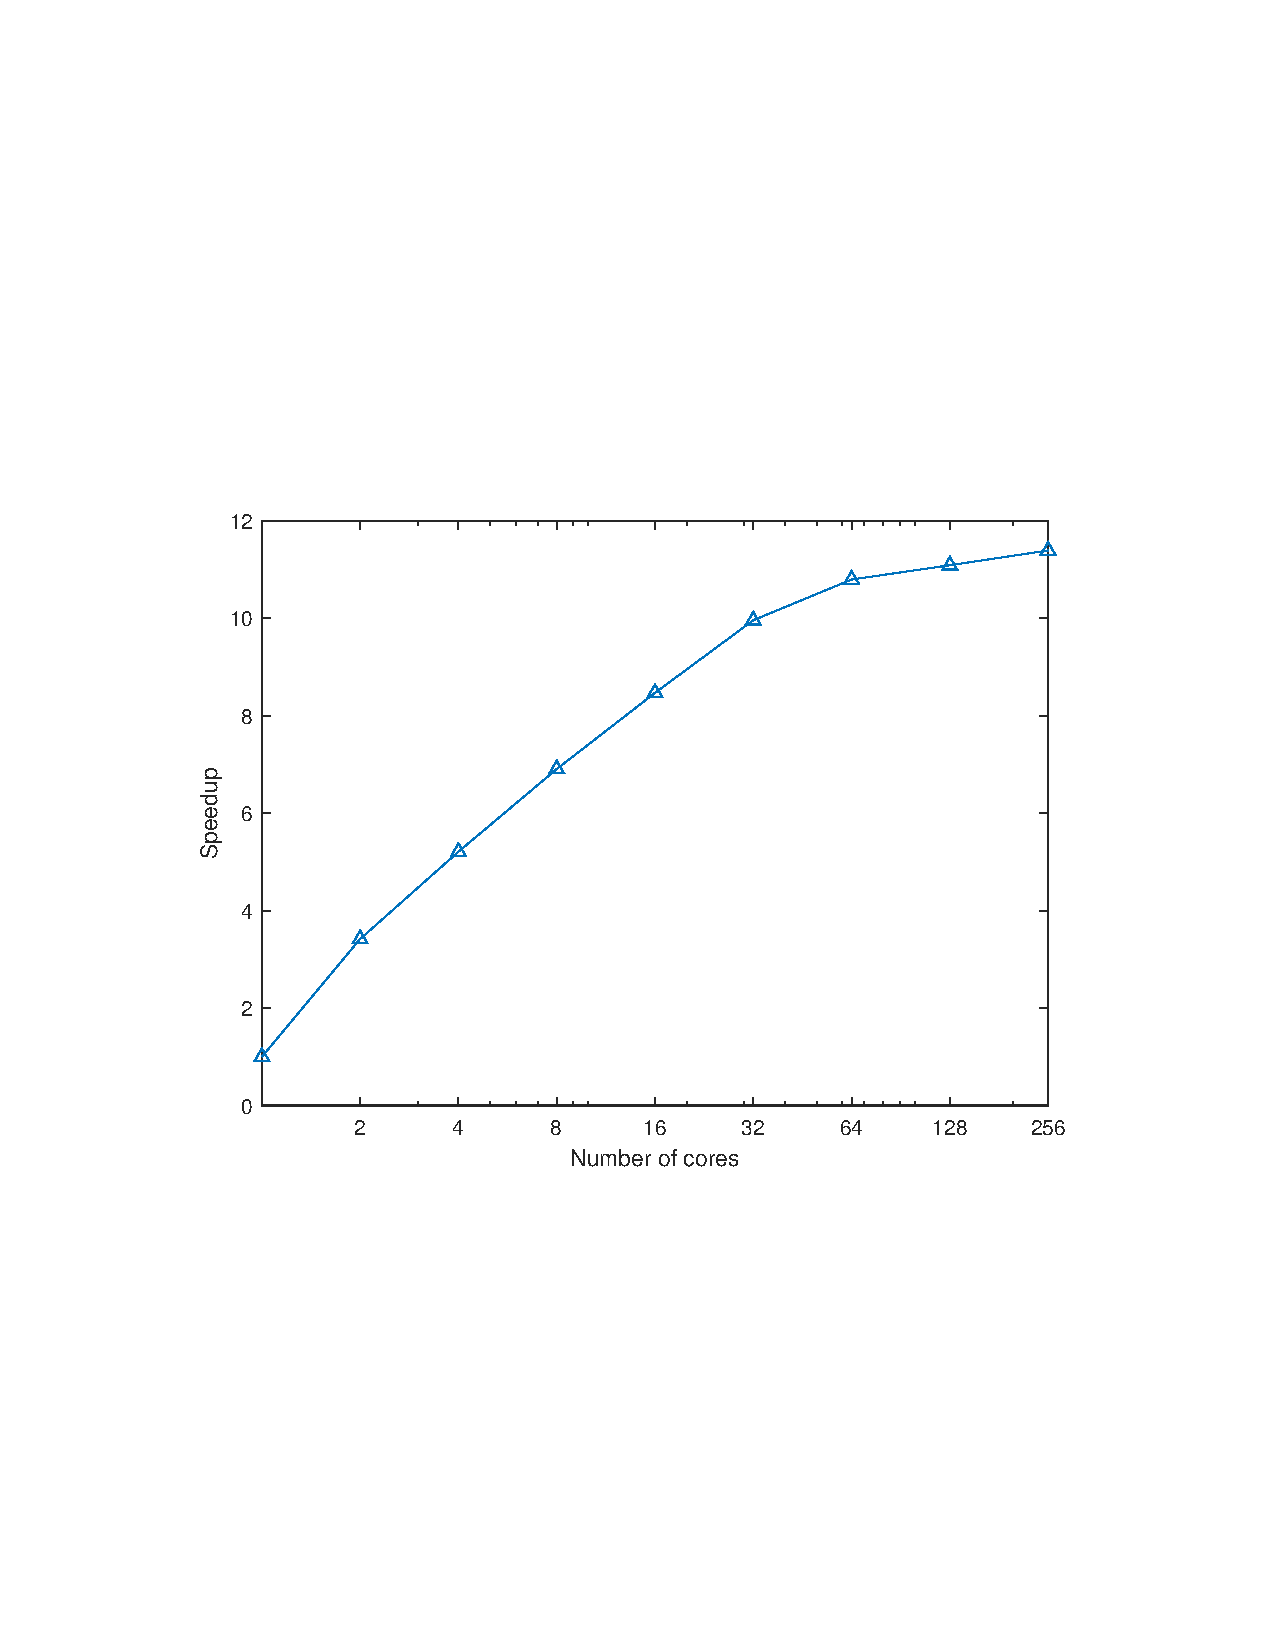
\includegraphics[scale=0.75]{rslsts_2mm_DEM_speedup_mtlb.pdf}
\caption{The speedup achieved in the DEM simulations of 2 mm particles. There 
was a linear increase up to 16 cores while the speedup seems to plateau when 
more number of cores are used due to larger amount of communications.}
\label{fig:rslts_DEM_speedup}
\end{figure}

\begin{figure}
\centering
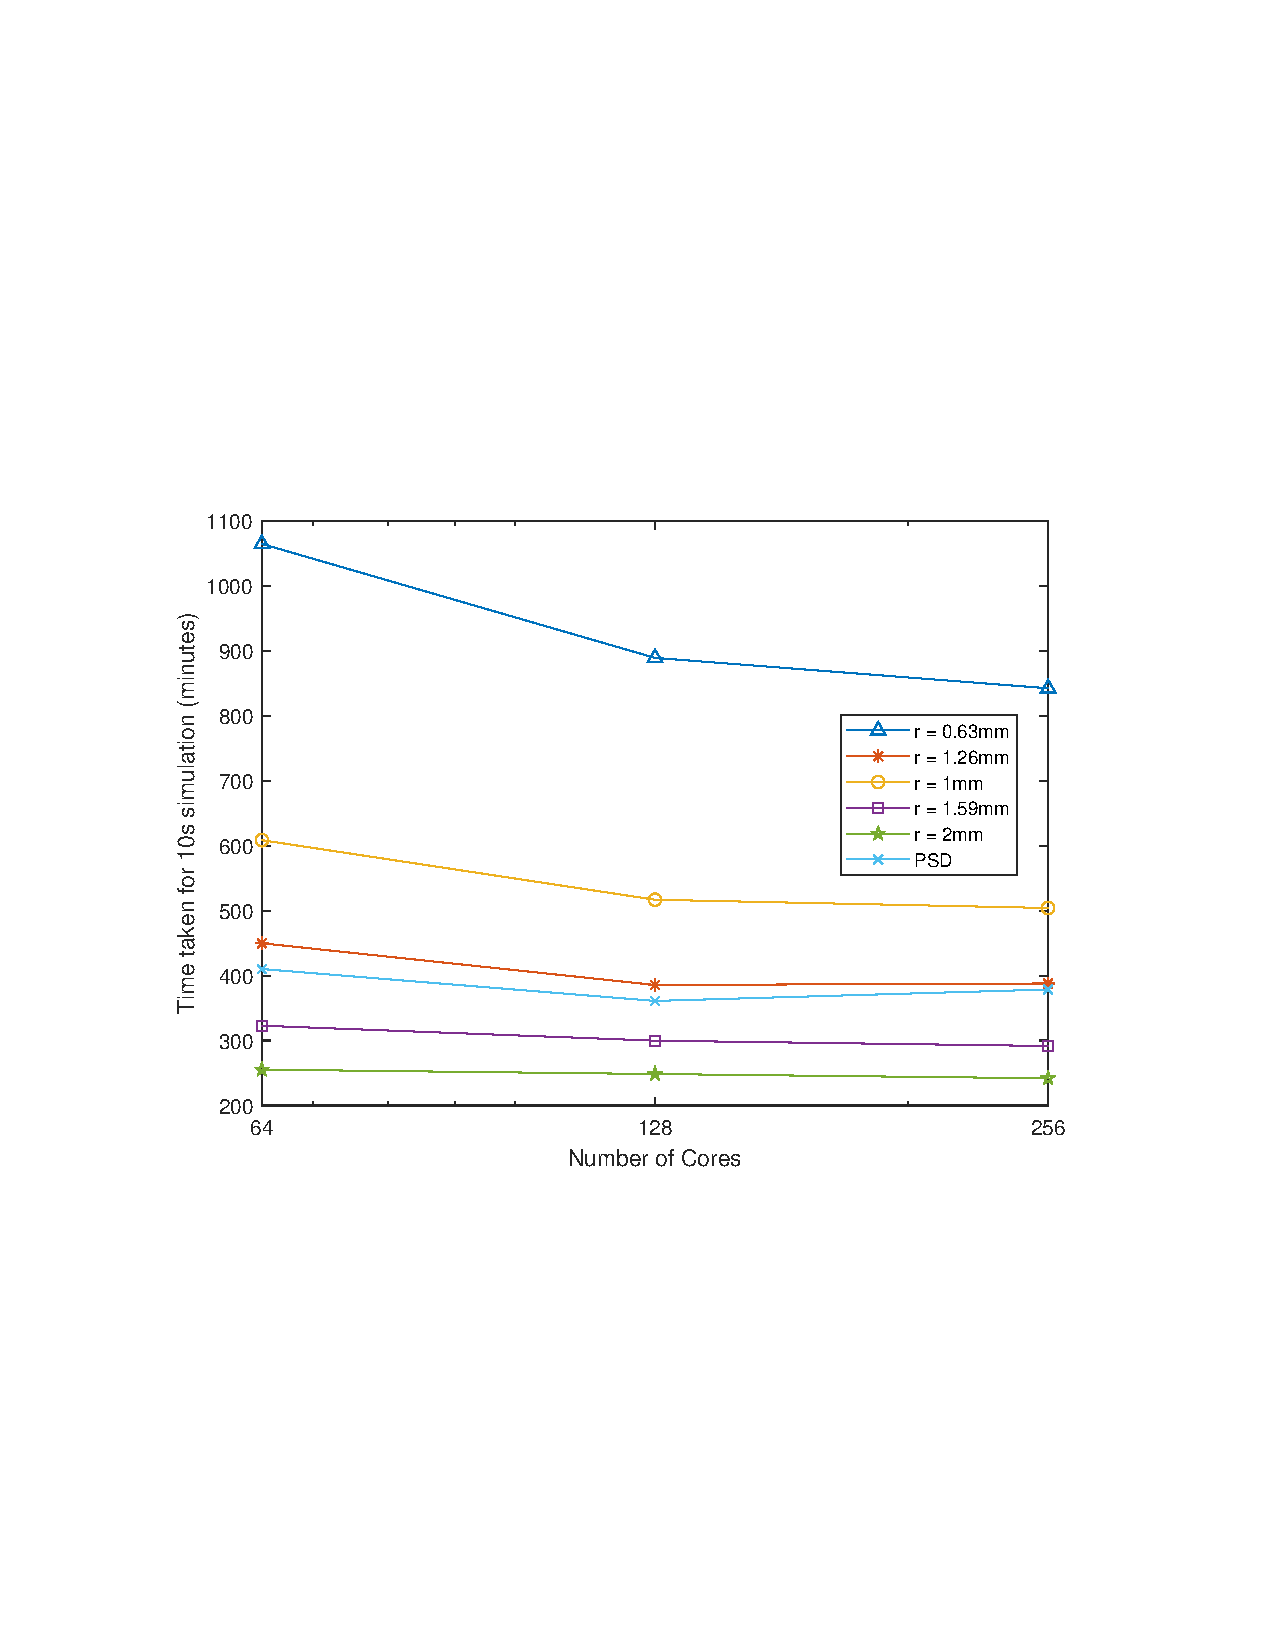
\includegraphics[scale=0.85]{rslsts_DEM_alldia_timing_mtlb.pdf}
\caption{ Time taken for a 10 second DEM simulation for radii ranging from
 0.63mm to 2mm and a particle size distribution ranging from 1mm - 3mm. The speed improvements 
 for the smaller particles was higher as the core count increased when compared to the larger particles. 
 The larger number of smaller particles require more computational power thus benefit more as the number 
 of cores are increased. }
\label{fig:rslts_DEM_timing_studies}
\end{figure}

The communication time in LIGGGHTS is indicated by the Modify time, which is the sum of the 
times required to transfer the rotating mesh from one process to the other. From Figure~\ref{fig:rslts_DEM_percent_plot}, it can be seen that the main portion of the simulation time is taken up by 
the modify time. This is expected since the impeller is rotating at a very high speed of 2000 rpm. So, if 
the number of processes are increased the amount of time spent in transferring the mesh also 
increases. In the studies, the modify time as a percentage of the simulation increased from 82\% to 
about 90\%, when the core count was increased from the 64 cores to 256 cores. But, the using the 
higher number of cores reduces time taken to calculate particle-particle interaction as well as in 
neighbor calculation. Thus, a better implementation for meshing as well as decomposition of the 
geometry for faster simulations with higher core counts.

\begin{figure}
\centering
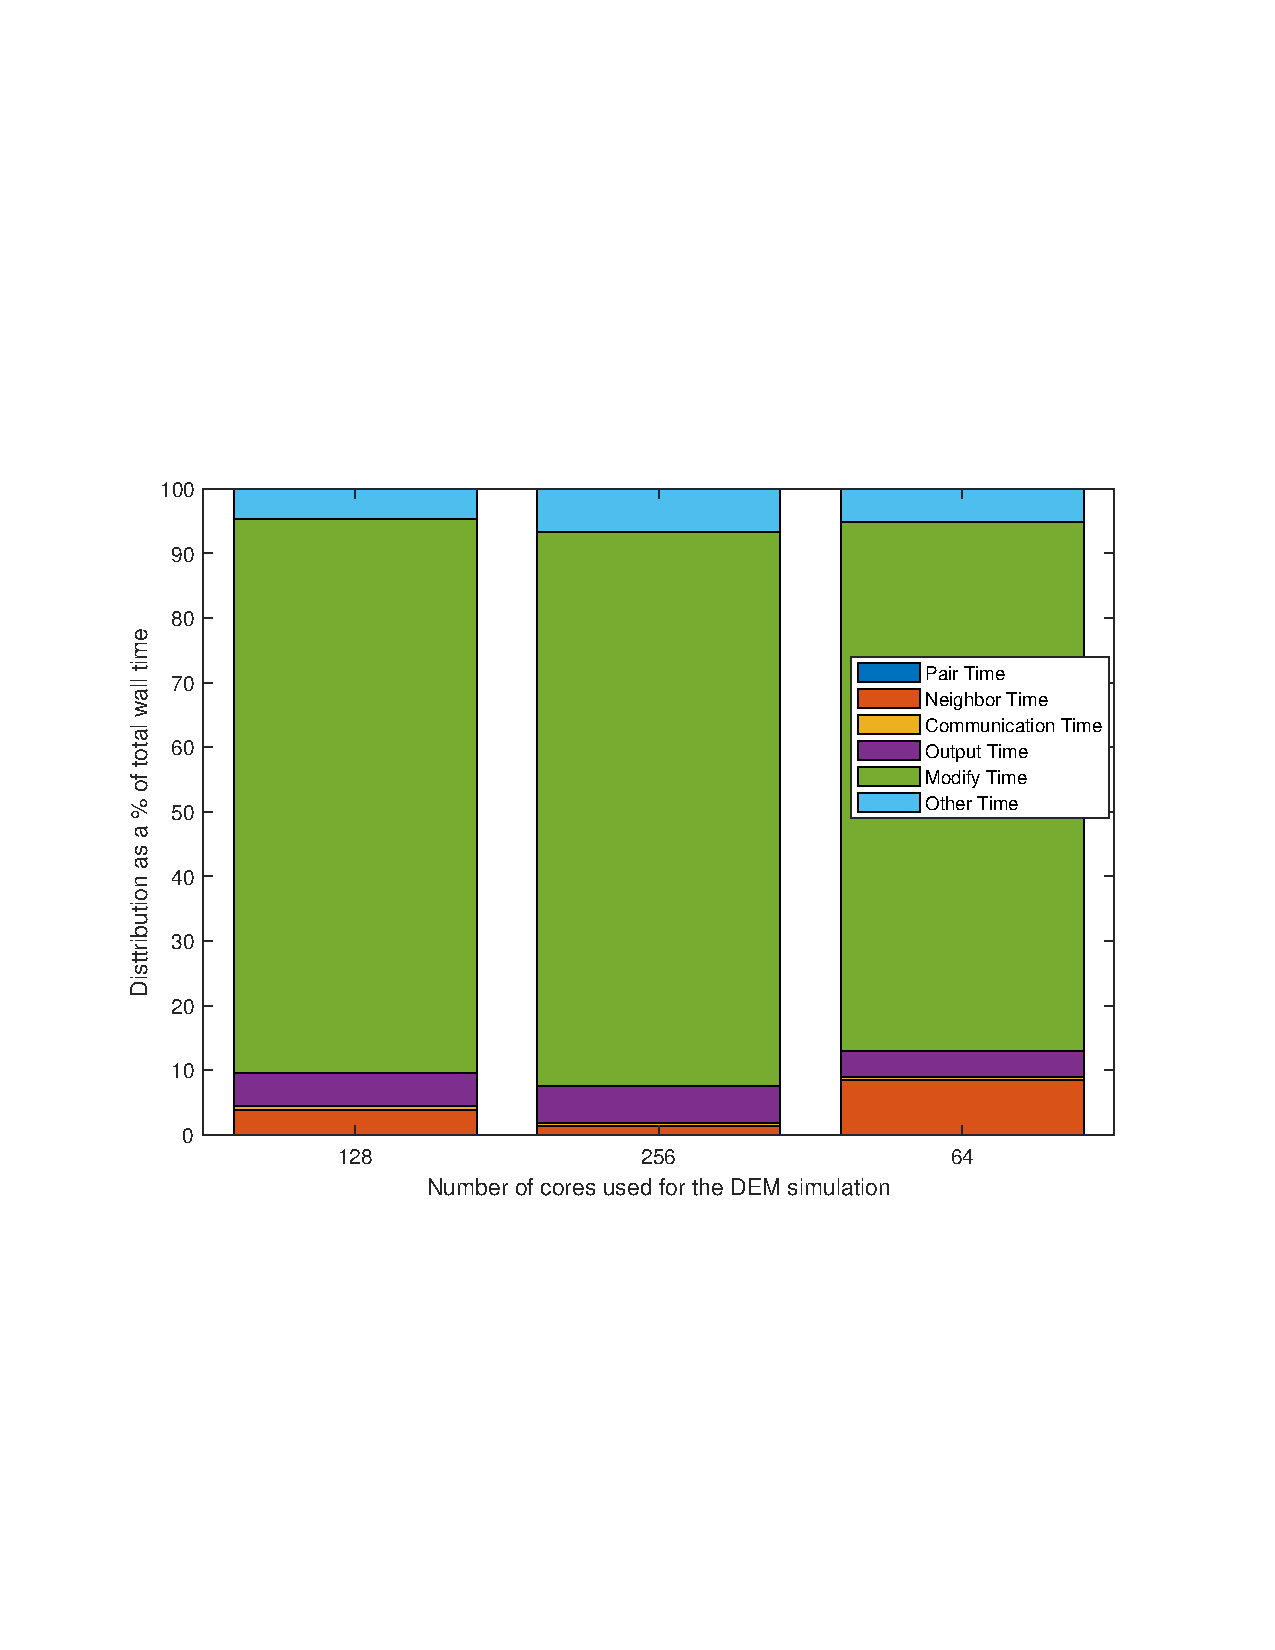
\includegraphics[scale=0.75]{rslsts_DEM_profle_mtlb.pdf}
\caption{The distribution of time taken by each component of the DEM 
simulation with varying number of cores for the 2mm particles. It 
can be observed that the percentage of time required to modify the 
geometry (indicated by the modify time), i.e. rotating the impeller 
at high speeds, was the highest.}
\label{fig:rslts_DEM_percent_plot}
\end{figure}


\subsection{Population Balance Modeling (PBM)}
\subsubsection{PBM model validation}
 The population balance model implemented was considered to have an inlet flow of particles in the 
first compartment at a constant mass flow rate of 15 kilograms per hour. The particles were assumed 
to have a log normal distribution with minimum diameter of the particles being about 12 $\mu$m and the 
maximum of 2.1 mm with a mean of 0.453 mm and a standard deviation of about 0.62 mm. \\
The PBM used in this study employs an aggregation kernel that takes into account the formation of a 
larger particle from only two smaller particles. The ratio of the rate of formation and the rate of 
depletion due to aggregation helps us monitor whether the PBM satisfies the conservation of mass. 
Since this PBM takes into account the aggregation of only 2 particles at once, the ratio of the particles 
is expected to have a value of 0.5 during the aggregation process. This ratio was reported by the PBM 
to be 0.5 throughout the simulation, validating the accuracy of the PBM used.

Figure~\ref{fig:rslts_PBM_d50_plots} shows four different particle size distribution plots at four 
different time instants. Figure~\ref{fig:rslts_PBM_d50_plots}(\subref{fig:30s}) shows the distribution of 
the particles at 30 seconds, where we expect to have the highest number of the smaller particles. 
Since the degree of aggregation that has occurred is very low, there is a jump in the number of 
particles of the smaller size. The particle size distributions at 2 intermediate times of 50 seconds and 
75 seconds are plotted in Figures~\ref{fig:rslts_PBM_d50_plots}(\subref{fig:50s}) \& \ref{fig:rslts_PBM_d50_plots}(\subref{fig:75s}) respectively. These illustrate that there is an increase in 
the number of larger particles  and a subsequent decrease in the number of smaller particles. 
Figure~\ref{fig:rslts_PBM_d50_plots}(\subref{fig:100s}) shows the distribution 
of the particle size at the end of the granulation process. It can be seen that the number of particles in 
the higher diameter bins have increased.

\begin{figure}
\begin{subfigure}{.5\textwidth}
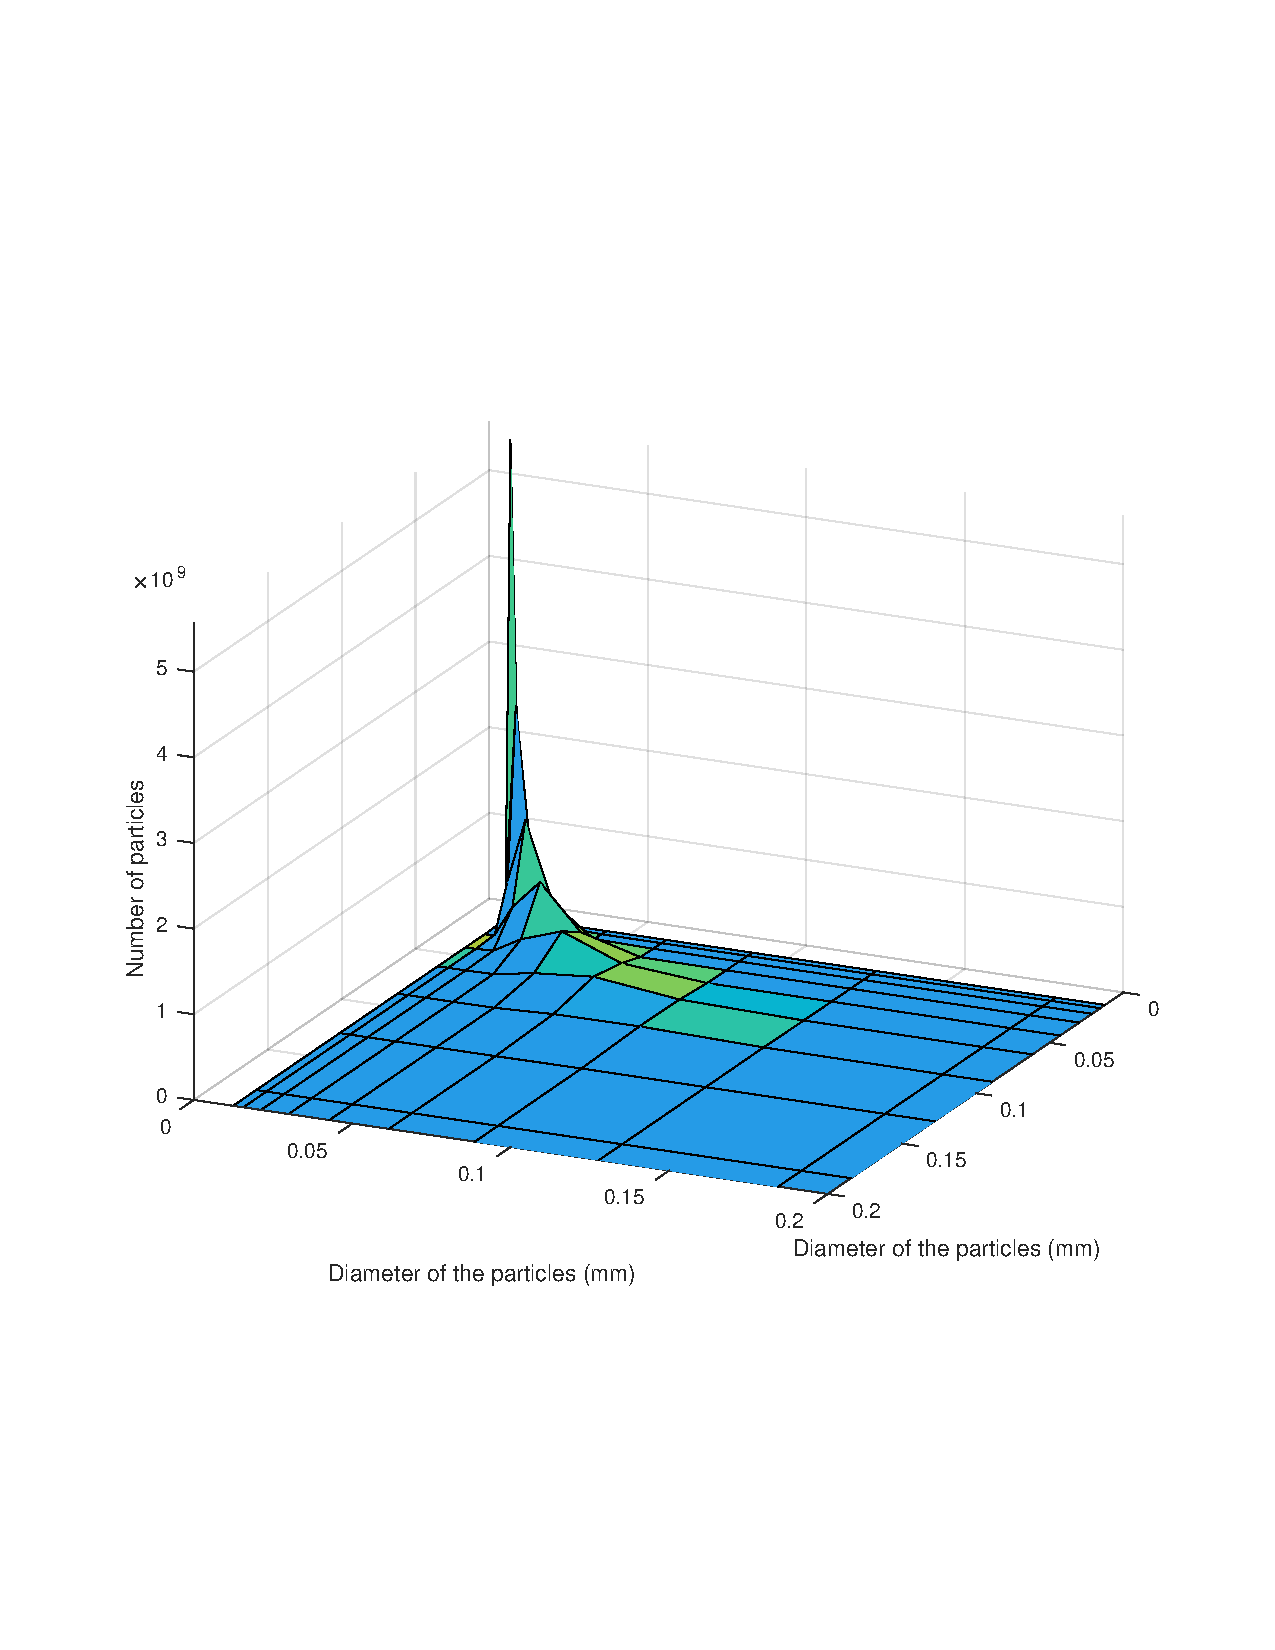
\includegraphics[scale=0.45]{rslts-PBM_30s_psd.pdf}
\caption{}	
\label{fig:30s}
\end{subfigure}\hfill
\begin{subfigure}{.5\textwidth}

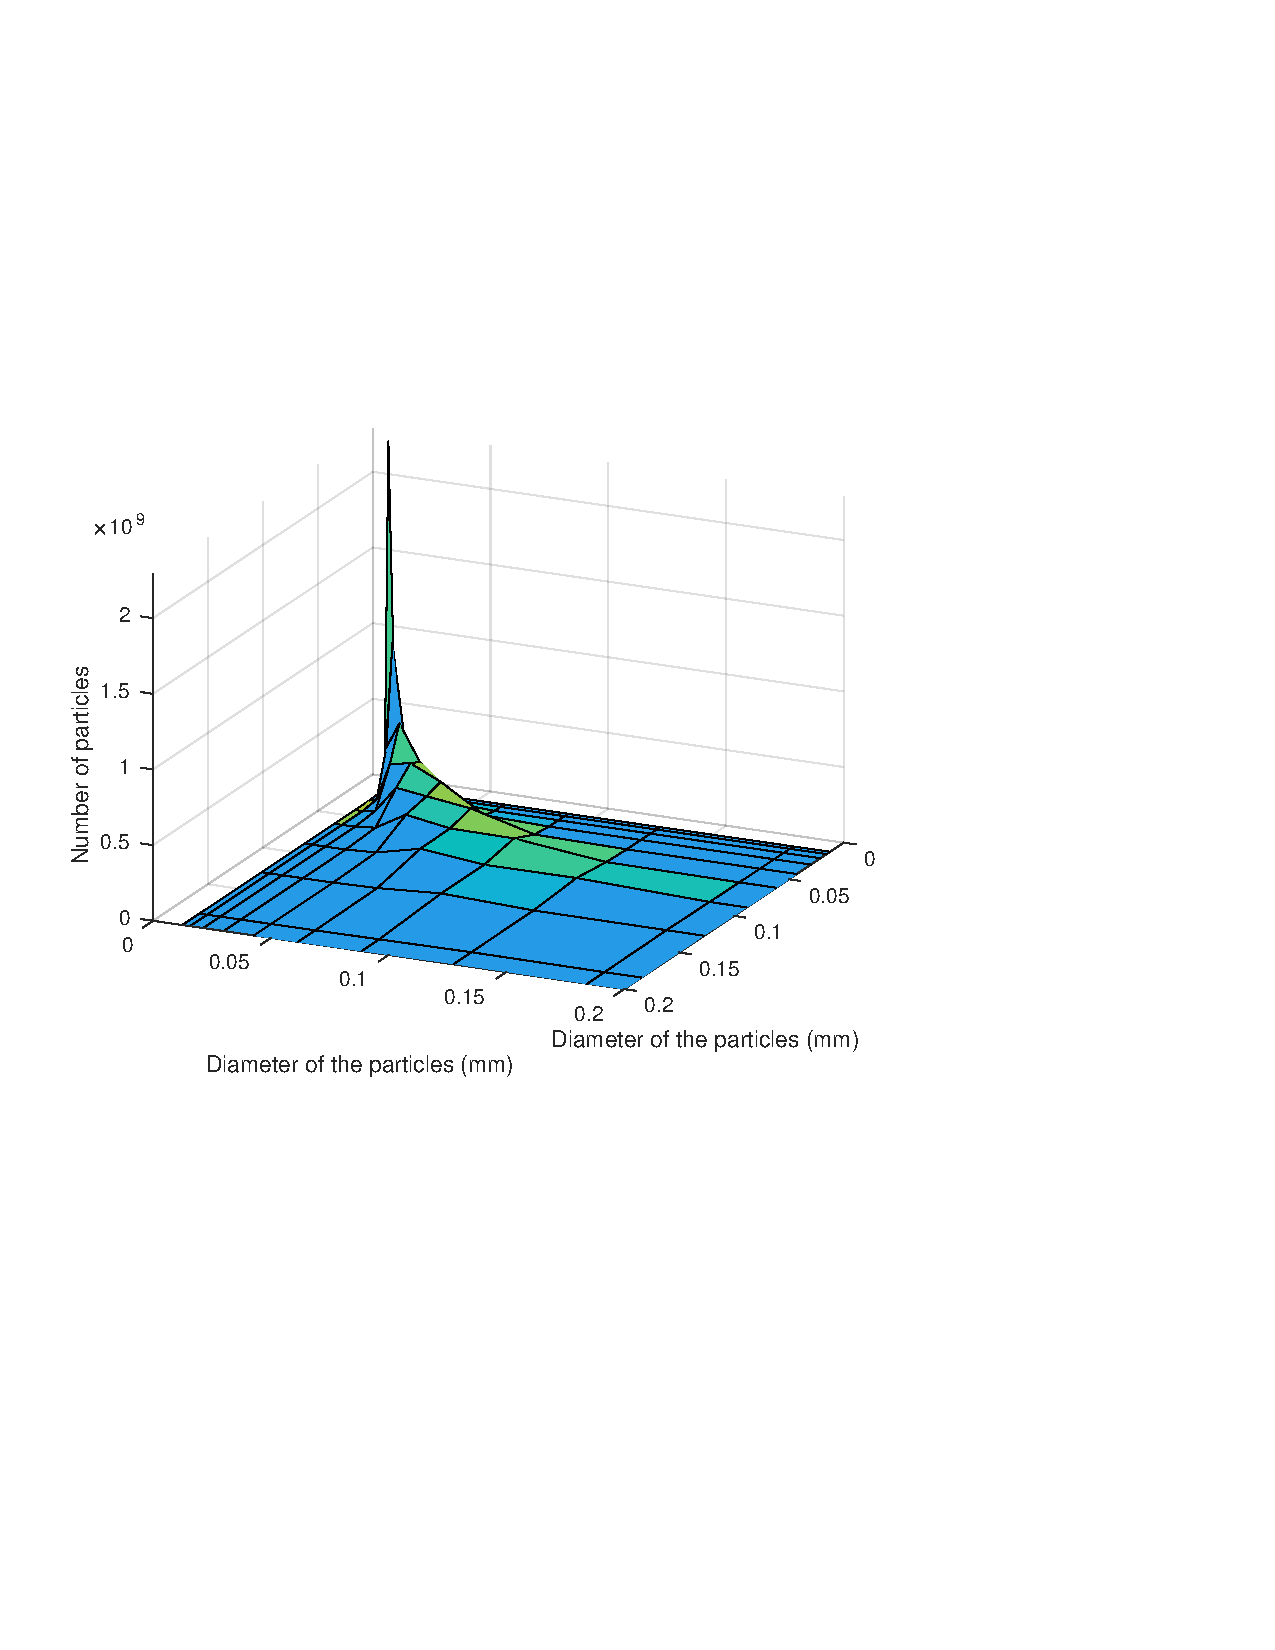
\includegraphics[scale=0.6]{rslts-PBM_50s_psd.pdf}
\caption{}
\label{fig:50s}
\end{subfigure}
\begin{subfigure}{.5\textwidth}

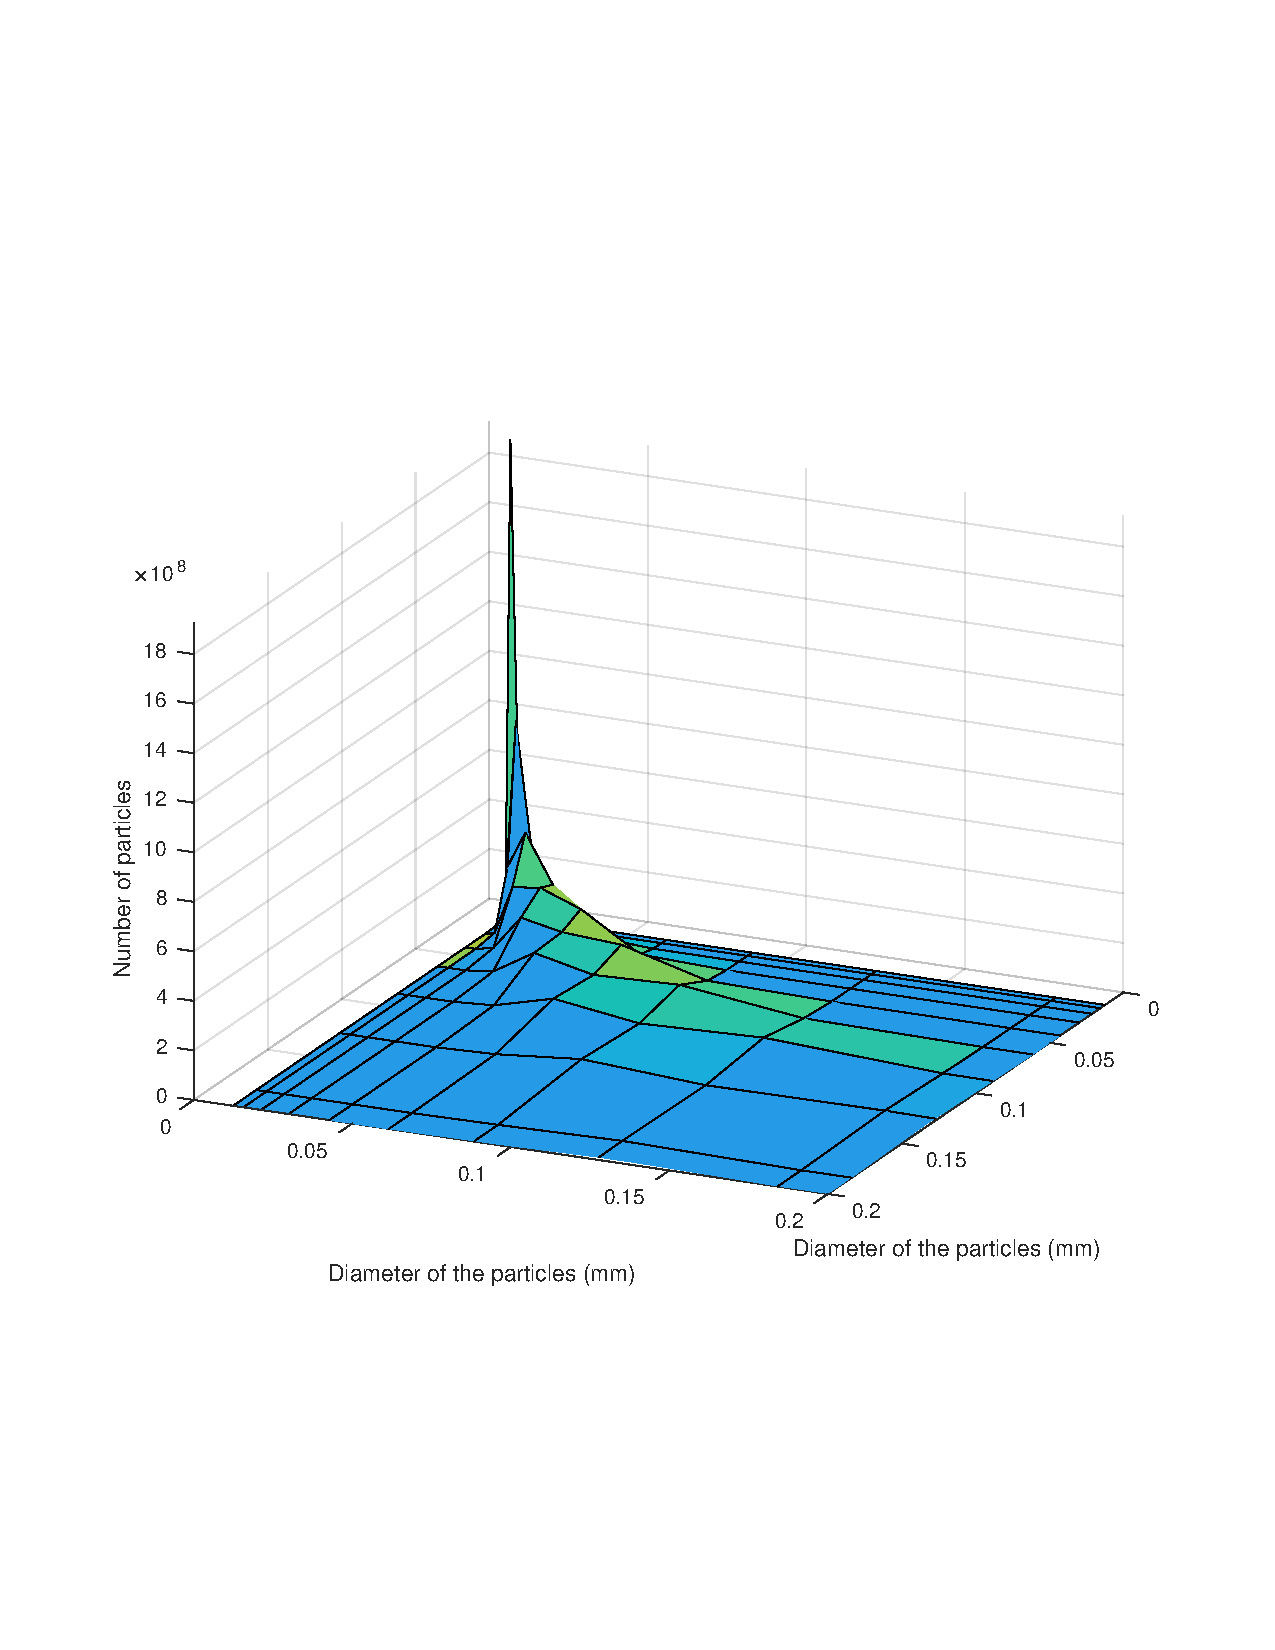
\includegraphics[scale=0.45]{rslts-PBM_75s_psd.pdf}
\caption{}
\label{fig:75s}
\end{subfigure}\hfill
\begin{subfigure}{.5\textwidth}

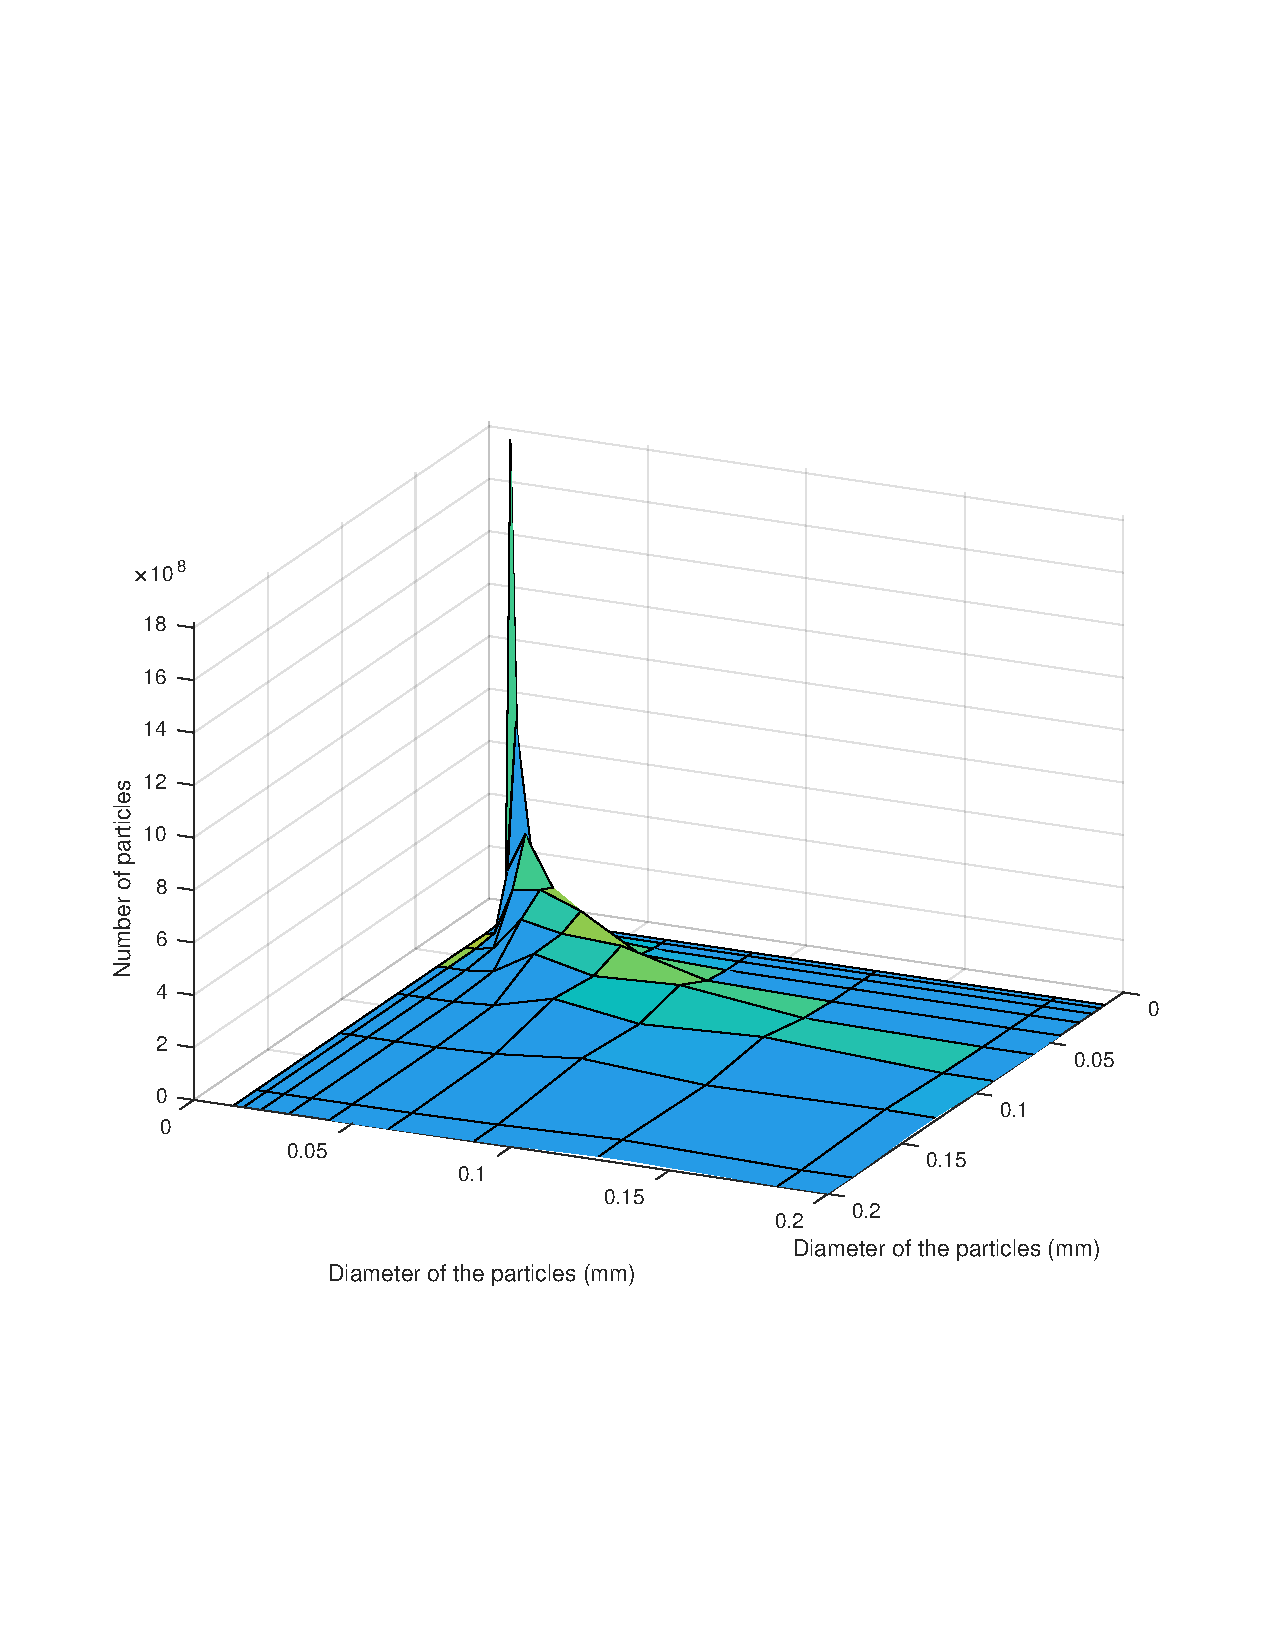
\includegraphics[scale=0.45]{rslts-PBM_100s_psd.pdf}
\caption{}
\label{fig:100s}
\end{subfigure}
\caption{ Representation of the total number of particles inside all compartments with diameters less than 0.2 mm 
in mm after (\subref{fig:30s}) 30s (\subref{fig:50s}) 50s (\subref{fig:75s}) 75s and
 (\subref{fig:100s}) 100s of PBM simulation (Mixing takes place for the first 25 seconds).}
\label{fig:rslts_PBM_d50_plots}
\end{figure}   

\subsubsection{Parallel PBM performance studies}
 The PBM was run for the results obtained from each of the aforementioned DEM simulations. 
Since the PBM has been parallelized using hybrid techniques, a combination of MPI and OMP cores 
were used to perform the simulations. Figure~\ref{fig:rslts_PBM_timing_studies} shows the average time 
taken by a PBM simulation for a total of 100 seconds of the granulation process, which includes 25 
seconds of the mixing time and 75 seconds of granulation time. The time taken for simulating all DEM 
scenarios by a single set of core configuration of in less than 10\% of each other, thus, an  average 
time for a single core configuration was used to illustrate the performance. 
These simulations were run in a varied configuration of cores ranging from 1 to 128. The cores were 
initially increased to 16 by increasing only the number of MPI processes. To increase the number of 
cores used, 8 OMP threads were employed for a configuration of 32(4 MPI  and 8 OMP), 64(8 MPI  and 8 OMP) 
and 128 cores (16 MPI  and 8 OMP). Figure~\ref{fig:rslts_PBM_timing_studies} shows that the program scales 
well to about 32 cores but then, the improvement in the performance is negligible. The scaling with the 
only MPI cores shows substantial increase in performance. \\
\begin{figure}[H]
\centering
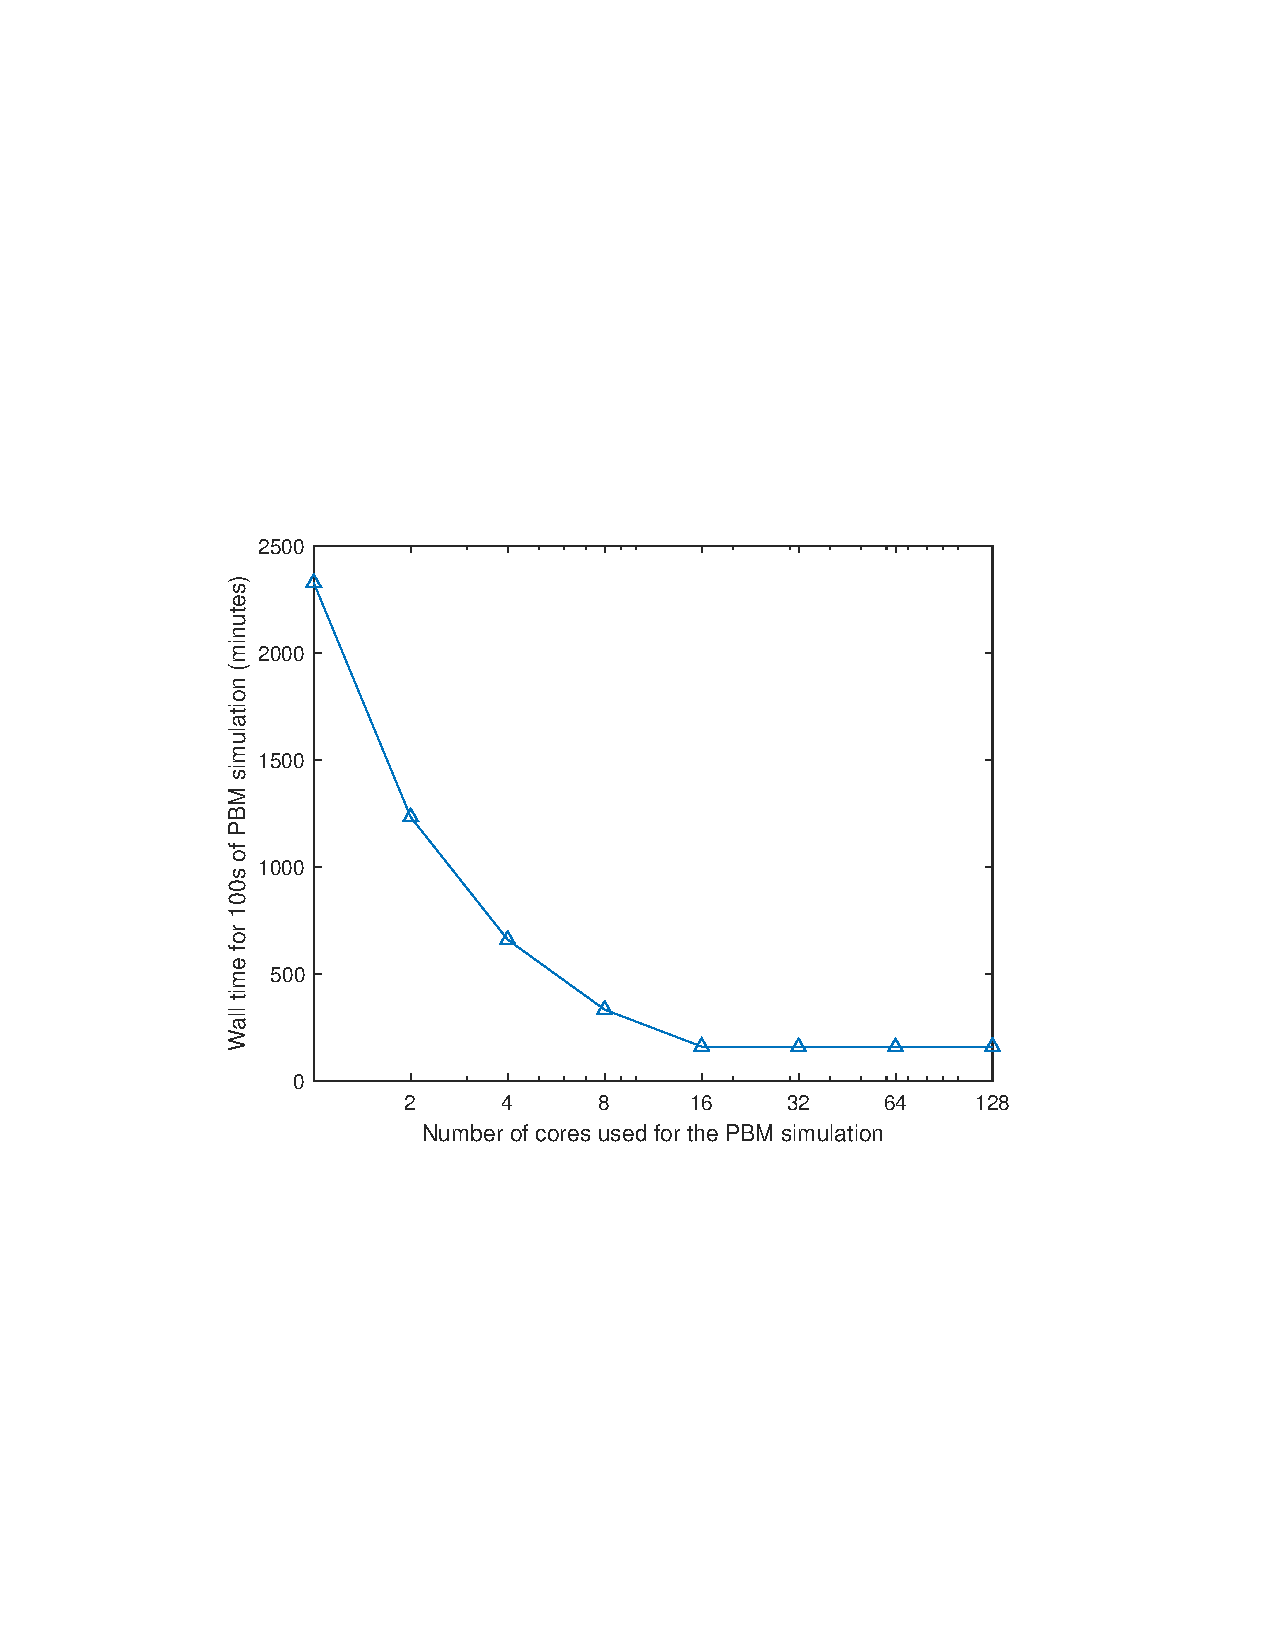
\includegraphics[scale=0.75]{rslsts_PBM_timing.pdf}
\caption{Average time taken to run the PBM simulation which consisted of 25 seconds of mixing time 
and 75 seconds of granulation time at different core configurations. There was a steady decrease as 
the number of MPI processes were increased, but the improvements on increasing the OMP threads were 
not that significant.}
\label{fig:rslts_PBM_timing_studies}
\end{figure}


Figure~\ref{fig:rslts_PBM_speed_up} depicts the speed up achieved by the hybrid parallel PBM code. It 
can be seen when the MPI cores used are increased from 1 to 16 cores the speed up achieved is 
almost linear. This speed can be accounted to the way MPI has been implemented inside the code. 
Each compartment of the granulator is  offloaded on one MPI process, thus making 16 MPI processes 
the ideal since, the granulator has been divided into 16 compartments. When less than 16 cores are used, 
more than 1 compartment is sent to a single MPI process, which leads to a 
decrease in performance. The implementation of OMP on top of the MPI parallelization helps improve 
the performance by the about 10\%. The calculations inside the OMP parallel section of the code 
consists of large number of nested loop which have been known to be difficult to parallelize~\citep{He2016} using the native \textit{C++}'s OMP libraries. The amount of communication time spent in 
between these threads is much higher than the speed increase achieved by using higher number of 
cores. One thread waits for another thread to complete processing the outer loops thus lower 
performance increase is achieved by using the OMP implementation. \\

\begin{figure}
\centering
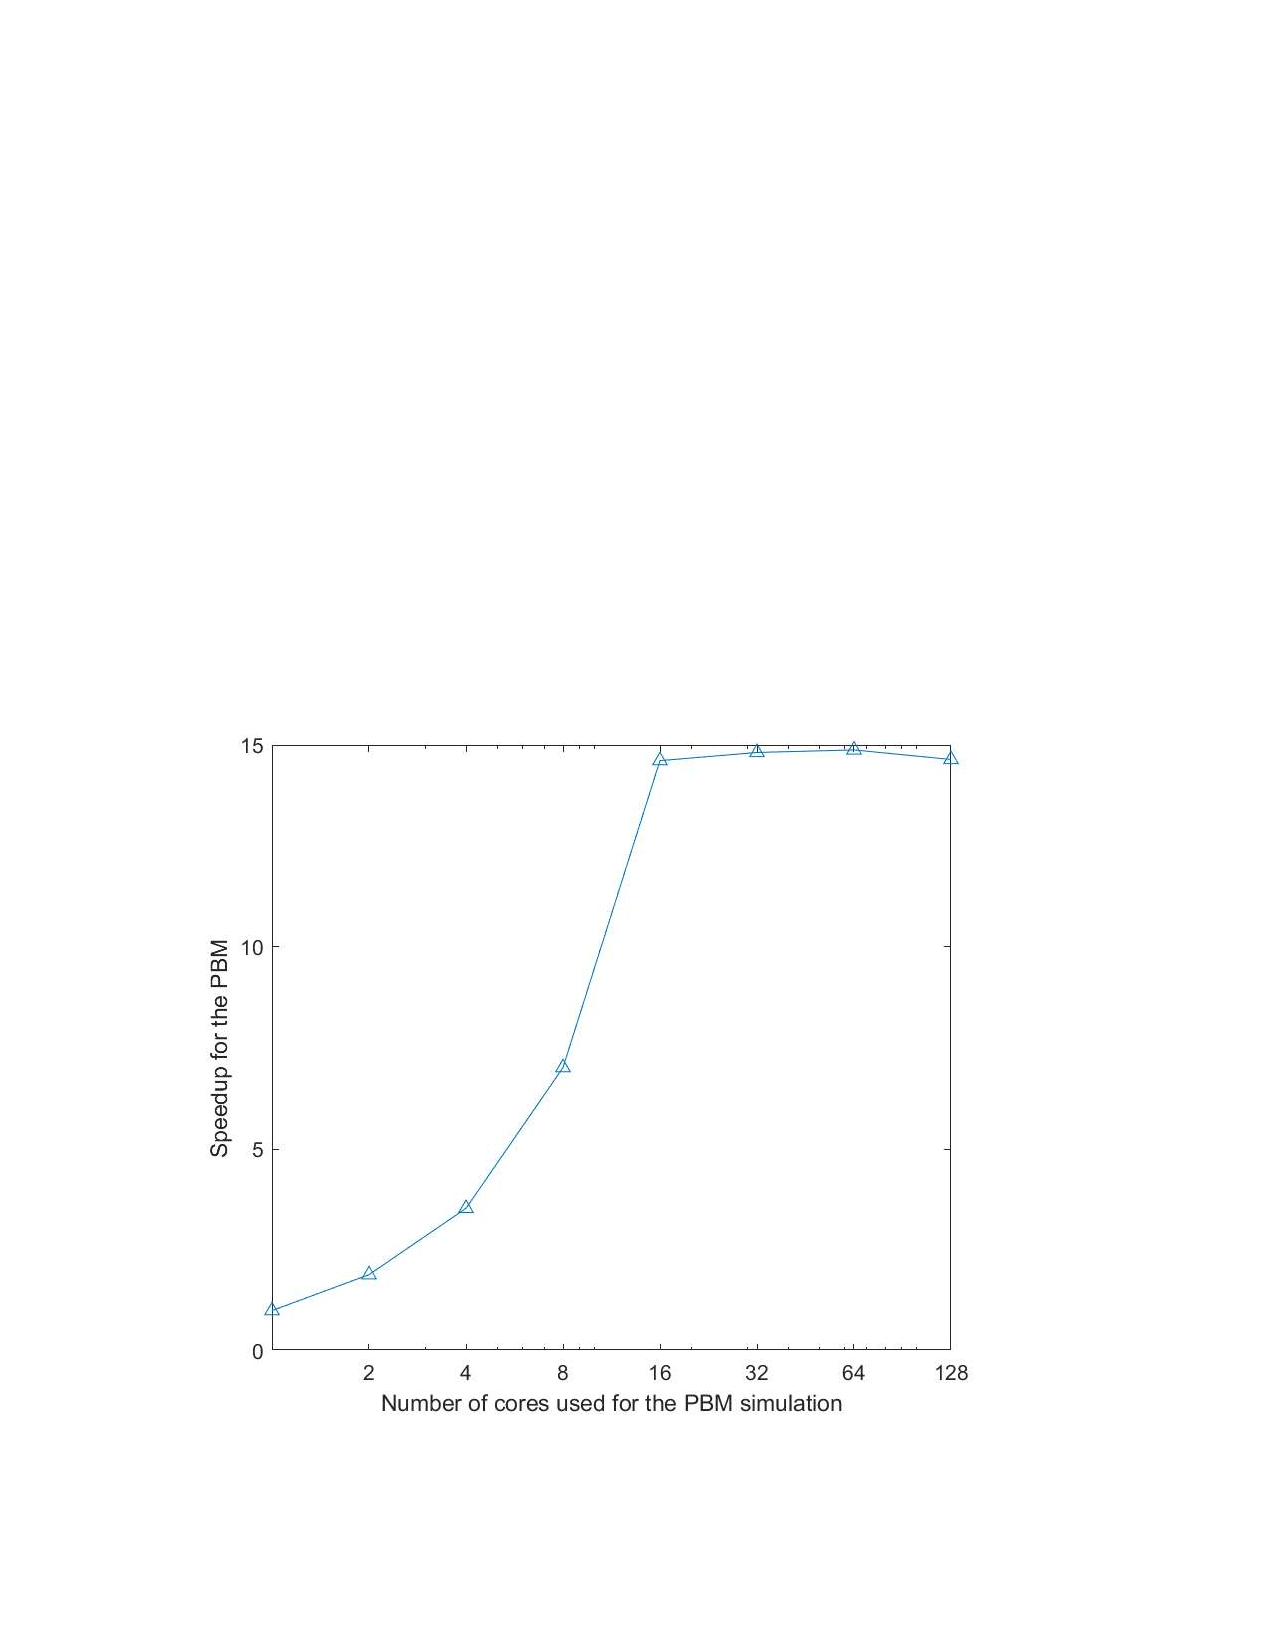
\includegraphics[scale=0.75]{rslsts_PBM_speedup_logx.pdf}
\caption{The speedup achieved by the hybrid parallel implementation of the PBM program. It can be 
seen the initial speedup up to 16 cores as expected as from an ideal parallel 
program where as it 
becomes almost constant from 32 cores to 128 cores}
\label{fig:rslts_PBM_speed_up}
\end{figure}

A similar behavior as in Figure~\ref{fig:rslts_PBM_parallel_efficiency} where the parallel 
efficiency of the program has been plotted against the number of the cores used. This efficiency 
decreases as the number of cores used increase. The decrease in efficiency initially up till 8 cores is steep as 
the communication time in between the MPI process decreases the efficiency, deviating its value from 
the ideal of 1 to about 0.4. With the increase in the MPI processes to 16 and then the 
implementation of OMP the efficiency decreases as there is no major increase in the performance 
when compared to the increase in the number of cores used. The efficiency falls to as low as 11\% 
when 128 cores are used. Thus, there is scope for improvement in the parallel implementation 
of the program using OMP, especially in section of the code where nested loops are present.

\begin{figure}
\centering
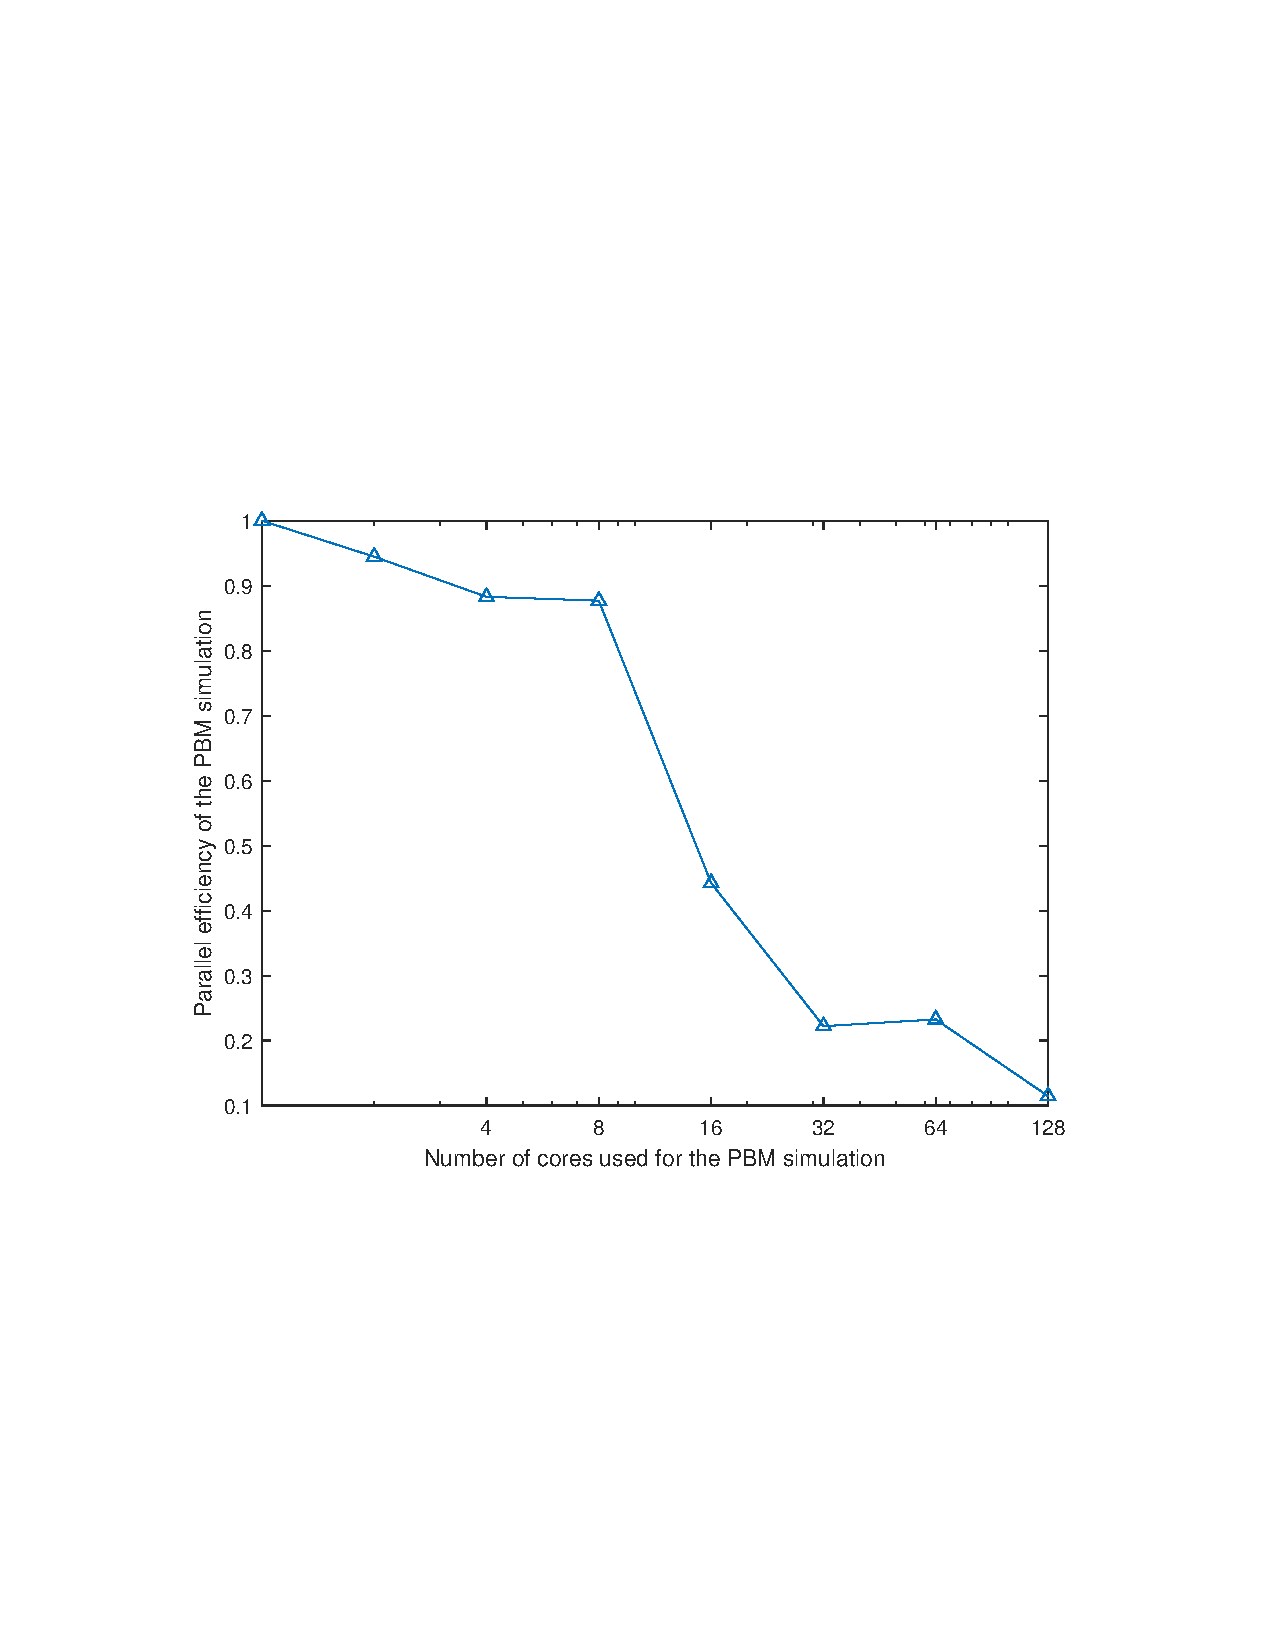
\includegraphics[scale=0.75]{rslsts_PBM_efficiency.pdf}
\caption{The parallel efficiency for the hybrid (MPI + OMP) parallelized PBM code. The efficiency of the 
code decreased as the number of cores are increased. The higher number of cores have very low 
efficiency of about 11\% which depicted that there is large time being spent in communication in 
between the cores.}
\label{fig:rslts_PBM_parallel_efficiency}
\end{figure}

\subsection{DEM + PBM physics}
The micro-scale simulations provide an insight about the physics of the system usually by tracking 
each particle. This micro-scale simulation data is useful for the development of macro-scale 
mechanistic models which take into account the dynamics of bulk of the particles and not individual 
particles. A similar approach has been implemented in this work, where a mechanistic aggregation 
kernel was developed from the DEM particle-particle collisions. Thus, the aim of this section is to 
illustrate that the physics of the system does not change to a great extent with the change in the size 
of the particles or the distribution of the particles.

Two simulations from the current scenario will be compared, the DEM + PBM simulation of the 2mm 
mono-sized particle and the second being the simulation where the inserted particles were in a size 
distribution. The ratio of rate of formation to the rate of depletion, both due to aggregation 
observed during these simulations was 0.5 which indicated that the PBM is stable. This meant that the
mono-sized and the PSD simulation were stable.

One of the metrics to determine the physics of the system after a PBM simulation is to check the 
median diameter (D\textsubscript{50}) plots of the system after the granulation process. 
D\textsubscript{50} indicates the maximum diameter of particles that constitute 50\% of the total mass. 
These diameters vary along the length of the granulator since the granulated particles take time to 
pass through the granulator and that there is not enough liquid content in the later sections of 
the granulator to encourage the formation of granules. Thus, the D\textsubscript{50} for compartments 
in the latter section of the granulator is low. Figures~\ref{fig:rslts_PBM_2mm_d50} \& \ref{fig:rslts_PBM_psd_d50} show the D\textsubscript{50} plots of the mono-sized and PSD respectively. 
It can be seen that both these plots have a similar behavior when it comes to the nature of the 
increase of the D\textsubscript{50} during the granulation process. There is a difference of about 
20\% in the final diameter of the particles predicted, which at the of micrometer scale does not affect 
the final product quality. This slight deviation is observed due to the sudden jump in the 
rate of the aggregation which increases when particles from one compartment with higher 
D\textsubscript{50} get transferred to the next compartment with a lower D\textsubscript{50}. 
The advantage of running the mono-sized simulation compared to the PSD simulation is the 
time taken to simulate the DEM. It can be seen from Figure~\ref{fig:rslts_DEM_timing_studies} that 
the 2mm mono-sized particle took about 1.6 times less than the PSD simulation time for the DEM. 
Since the physics of both the systems are not different, using the mono-sized simulations 
for the DEM help save time on the overall simulations. 

\begin{figure}
\centering
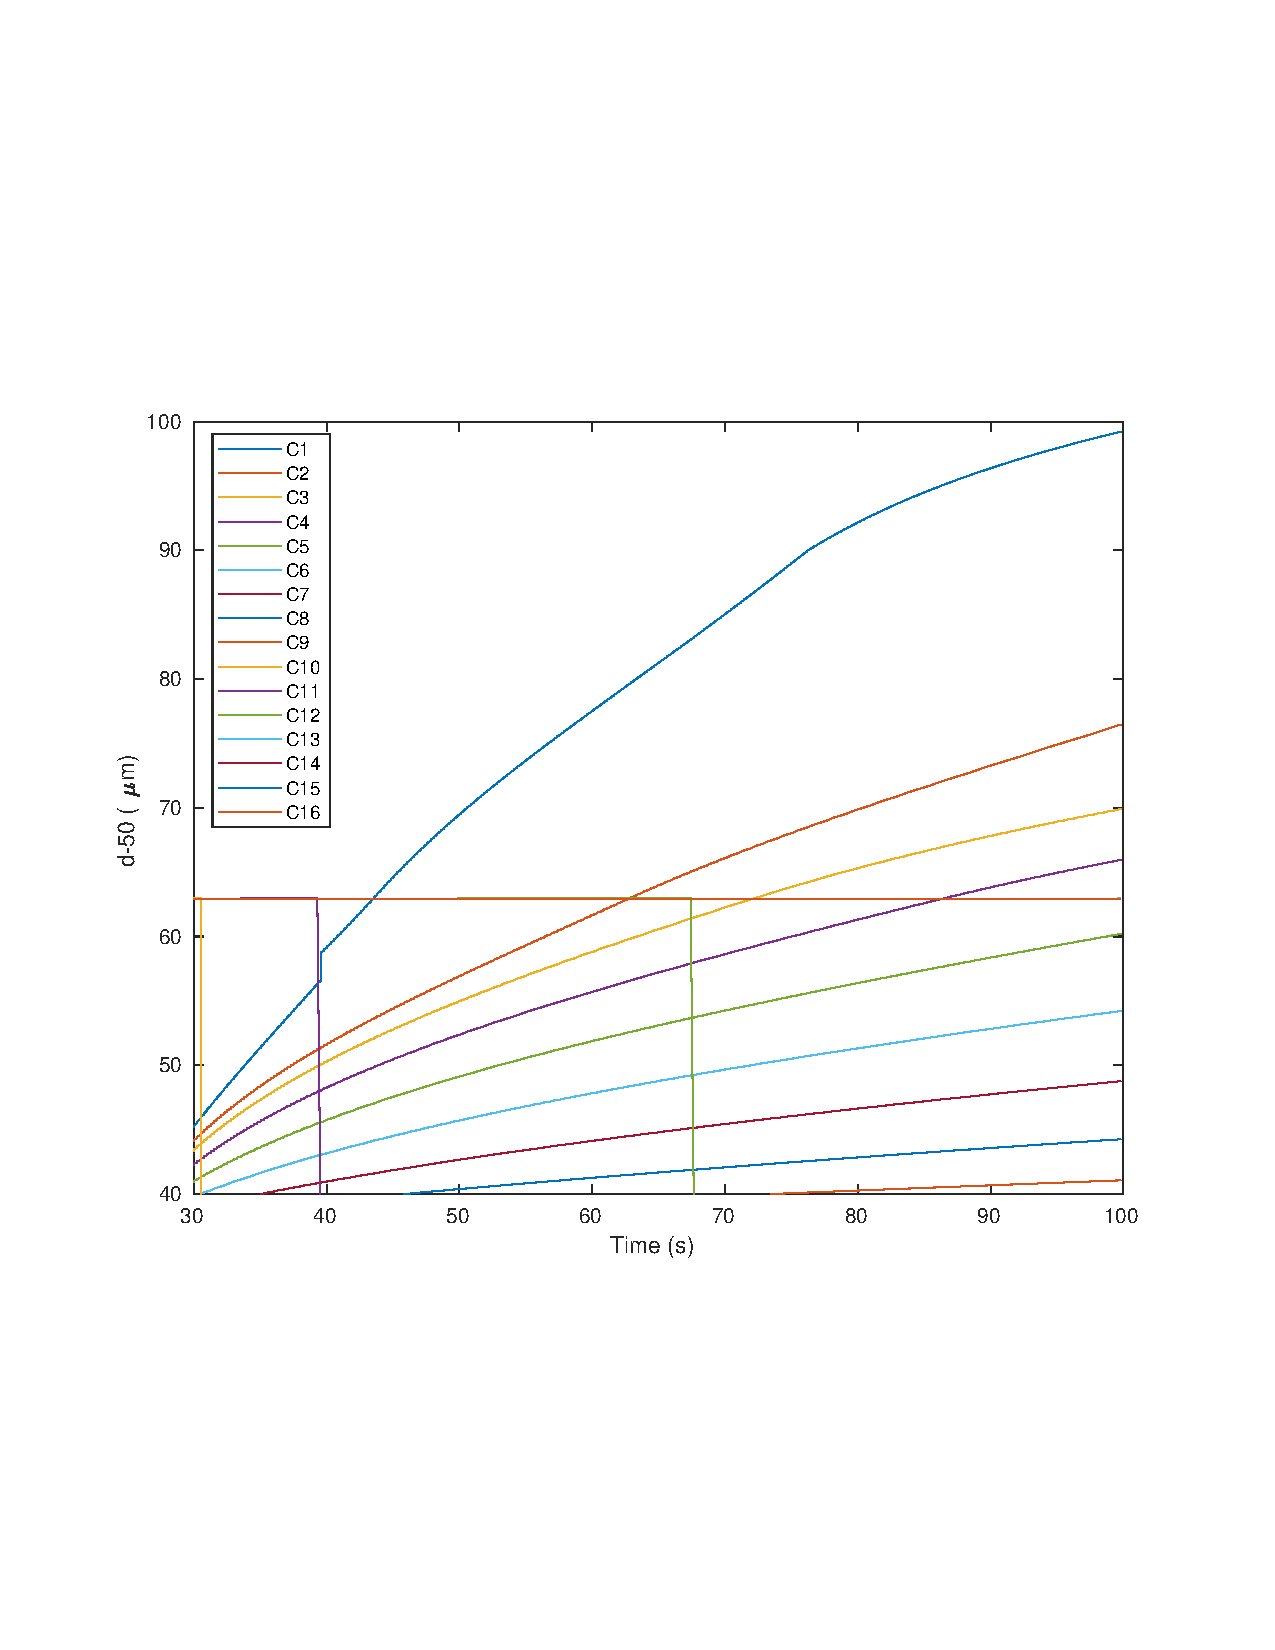
\includegraphics[scale=0.5]{rslts_pbm_d50_128_200.pdf}
\caption{D\textsubscript{50} of the particles obtained after 100s of granulation time (25s of mixing and 75s of 
liquid addition) for the 2mm mono-sized particle DEM simulation.}
\label{fig:rslts_PBM_2mm_d50}
\end{figure}

\begin{figure}
\centering
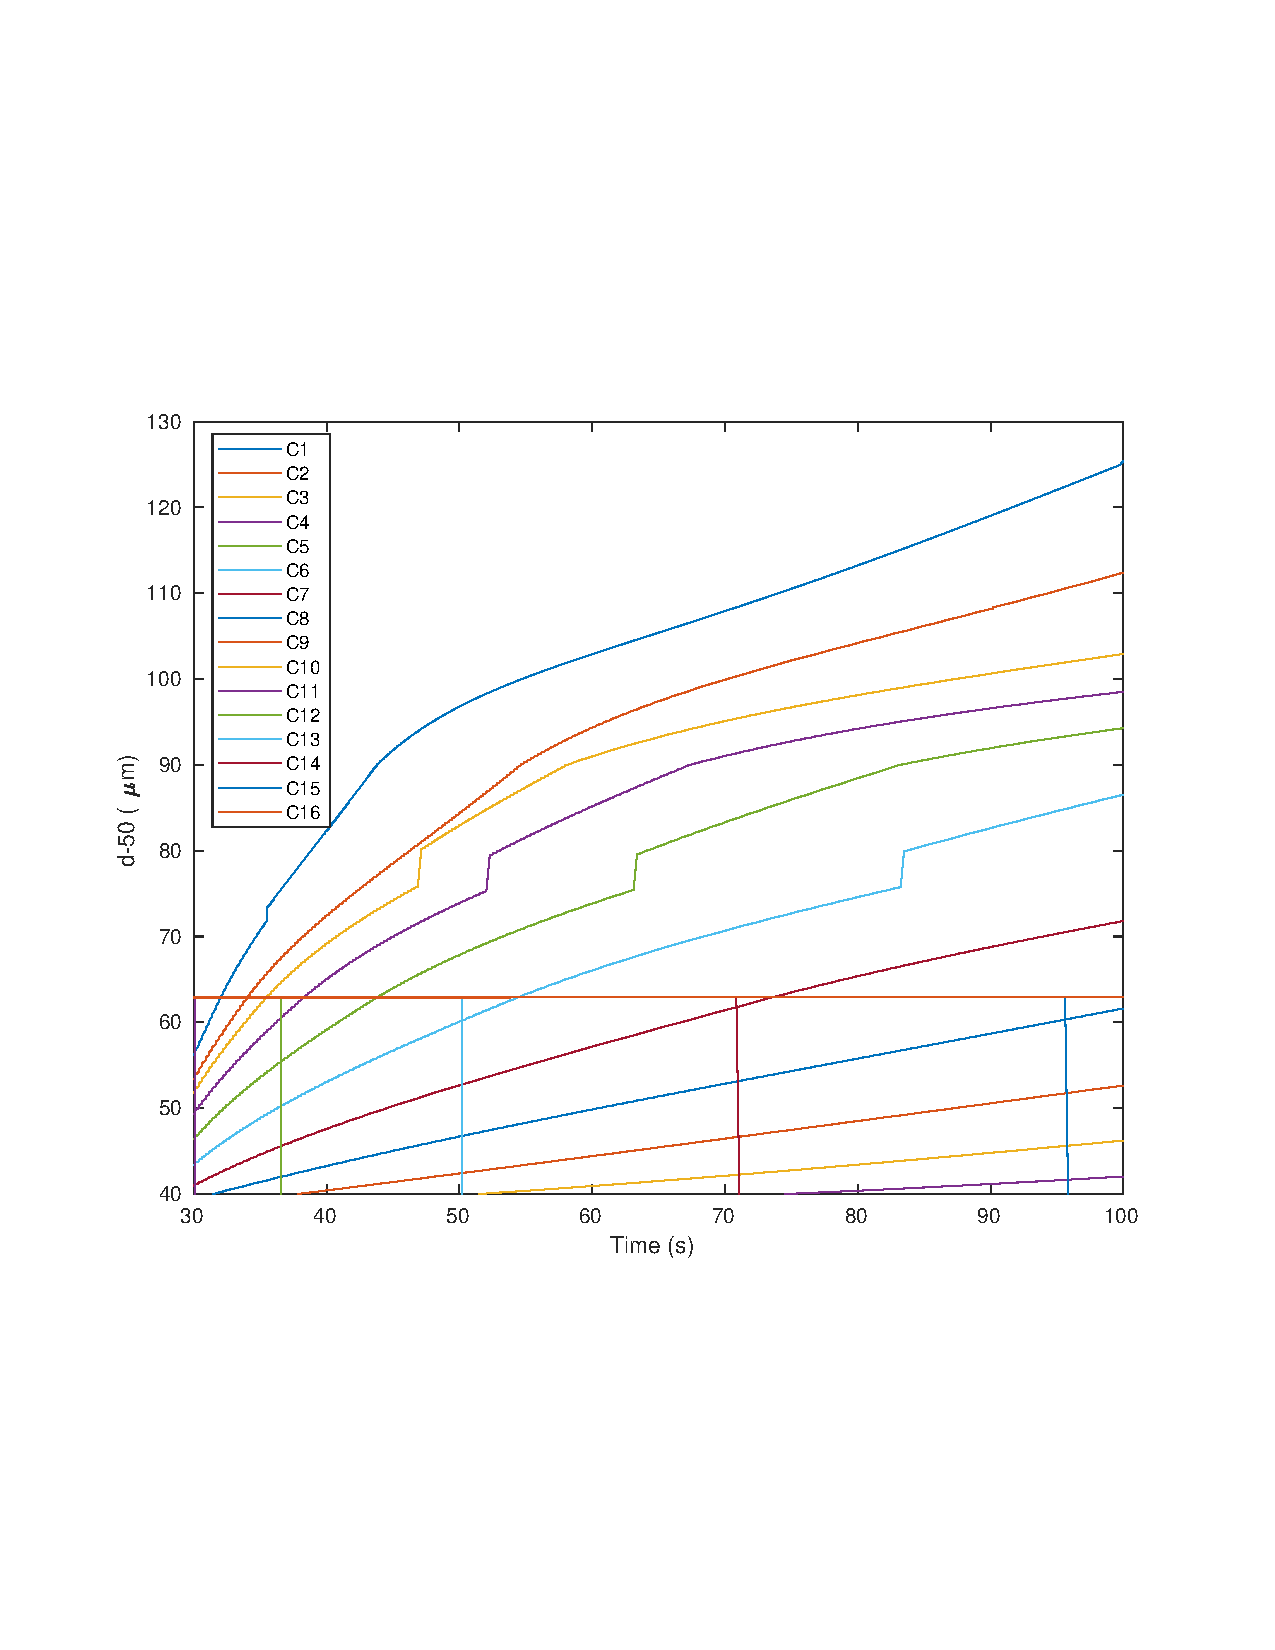
\includegraphics[scale=0.5]{rslts_pbm_d50_128_555.pdf}
\caption{D\textsubscript{50} of the particles obtained after 100s of granulation time (25s of mixing and 75s of 
liquid addition) for the distributed particle size DEM simulation. The trend observed was similar to the trend 
found in Figure \ref{fig:rslts_PBM_2mm_d50}}
\label{fig:rslts_PBM_psd_d50}
\end{figure}


\subsection{One-way coupled DEM+PBM using RADICAL-Pilot and its performance} 

The RADICAL pilot (RP) being a pilot job system it can bypass the need of
waiting on the long scheduler queues on a cluster. \jhanote{This is wrong! It
avoids the individual tasks from waiting for different periods of time at the
scheduler, not waiting itself at the scheduler!} With resources allocated to
itself the pilot can execute multiple simulation runs at once. The pilot job
initiates the DEM simulation using the LIGGGHTS executable compiled for the
DEM studies and then creates a link between the collision data obtained, which
is utilized by then utilized by the PBM executable. After the link is
established, it also initiates the PBM. The timing profiles and results from
both the simulations are then obtained. Since the executables and inputs files
used in the simulations and the RP job are the similar, we do not expect to
see any changes in the physics of the system. A value of 0.5 was obtained for
the ratio of the rate of formation to the rate of depletion due to aggregation
due to aggregation.

Since the platforms used for initial development and testing of the DEM and
PBM respectively were different, the DEM simulations were executed again on
Stampede2 for a fair and accurate comparison. The need for re-running the
simulations arises due to the clock speeds of the nodes and their
configuration for the 2 platforms is different. The RADICAL-pilot was setup
for Stampede2 and aforementioned experiments were replicated. The DEM
simulations were run for 64, 128 and 256 cores (MPI processes) and the PBM was
run for 1, 2, 4, 8 and 16 MPI processes. No OMP threads were implemented for
the PBM run, since the current version of RP does not support threading. The
times for the individual DEM and PBM simulations were added to determine the
total amount time taken to simulate the one-way coupling. This time did not
include the time spent by each executable in the queue of the scheduler. This
time could vary from a few hours to a few days depending upon the load of the
cluster. The total time taken for the simulation using the RADICAL-pilot was
determined from the time the DEM was first executed until the PBM execution
completed. The time of the individual DEM and PBM simulation was added to get
the total amount of time it required for a single one-way coupling simulation.
Figure~\ref{fig:rslts_RP_time_plot} shows a comparison of the total times of
simulation in seconds for the sum of DEM and PBM individual simulations to the
times taken to run the simulation using RP. It can be observed that the times
taken by the pilot job are slightly higher than the summation of times of the
individual simulations. The slight increase in the times of the simulation can
be accounted for by the communication required for the pilot to realize that the
DEM simulation has completed and link the data from the DEM to the PBM
executable before it is executable. But, this communication is lower than the
amount of time the executable the job would spend in the job scheduler queue.
Thus, the benefits of using RP become clear. \jhanote{It is unclear what the
benefit is!} An extension of this work would be to use RP to schedule multiple
such coupled simulations as one job, thus decreasing the wait times even
further.
\begin{figure}
\centering
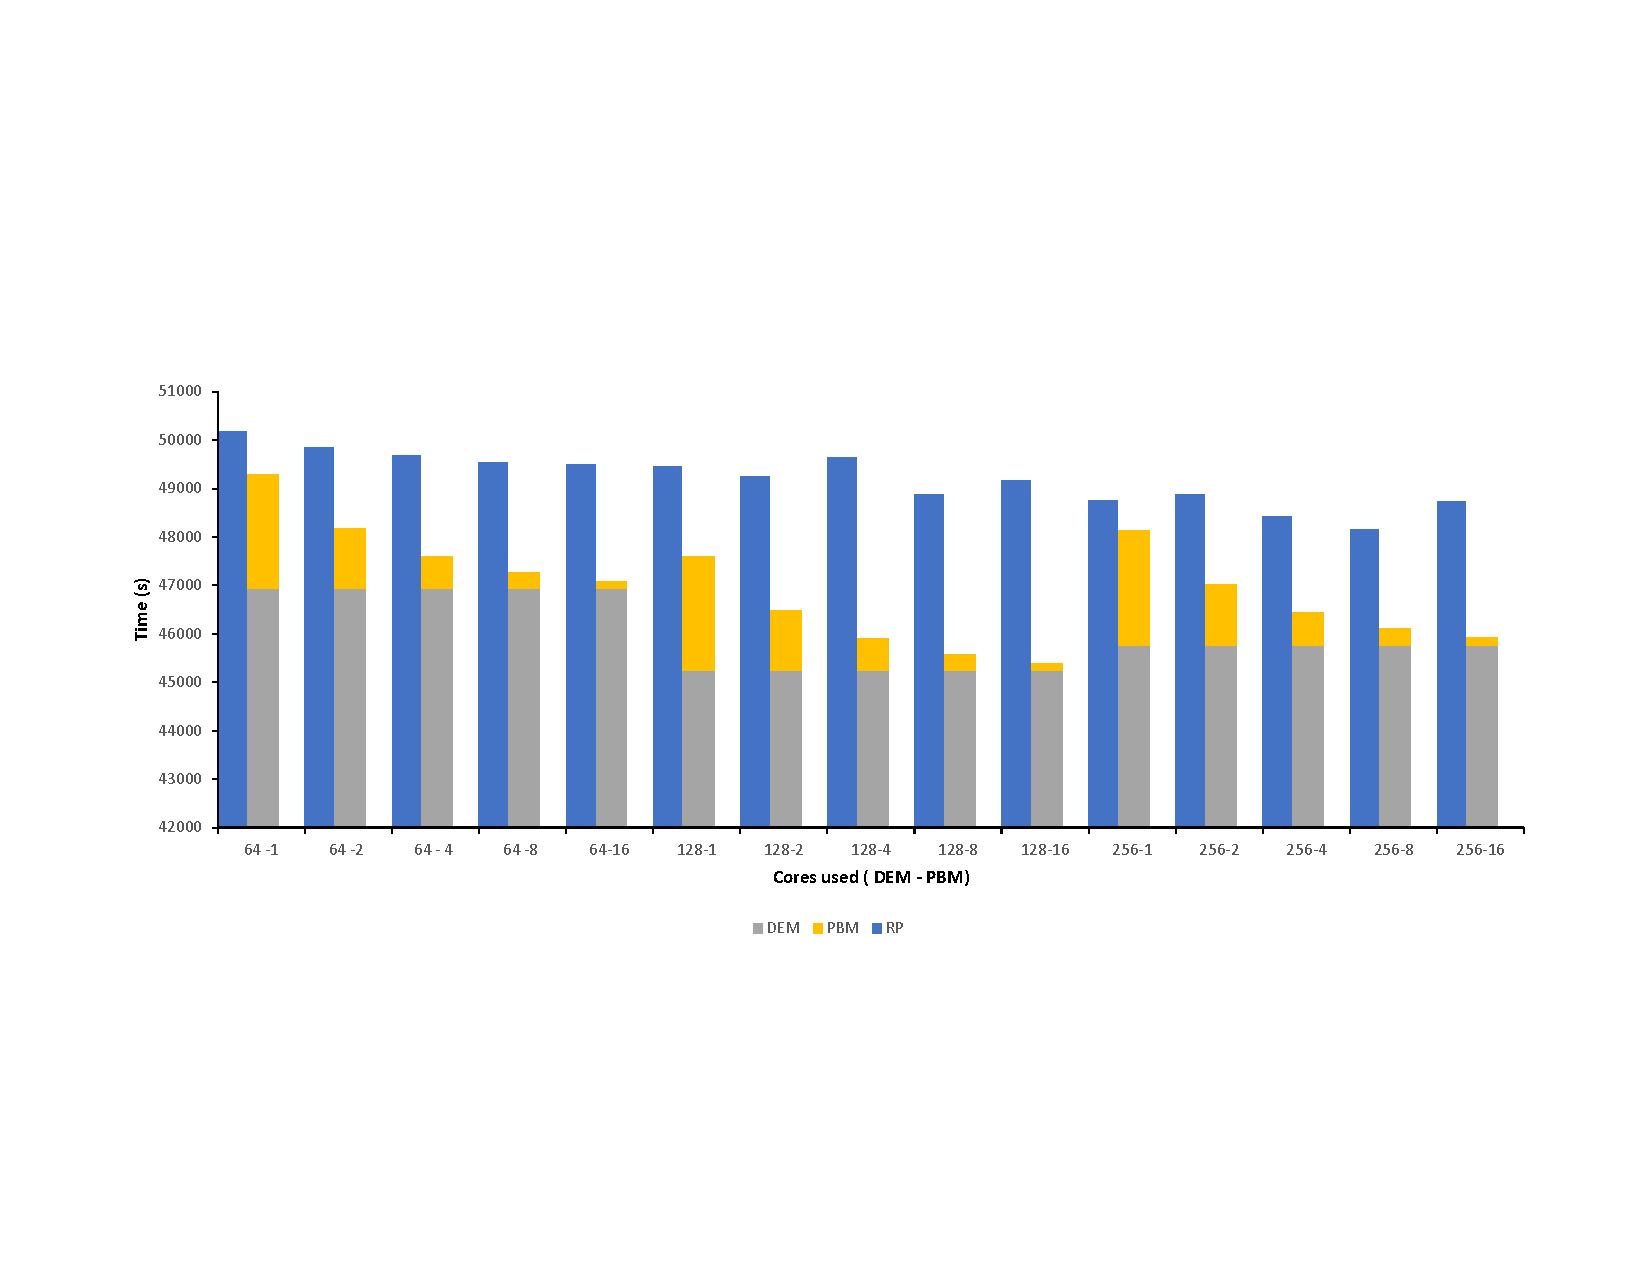
\includegraphics[scale=0.7]{rslts_RP_timeComparison.pdf}
\caption{A comparison of times taken by 2 individual simulations (DEM + PBM) (without 
including queue time) to the  time taken by Radical-Pilot to complete the same set of simulation. 
A slight increase in the time of the simulations was observed making RP a more convenient 
tool to perform simulations where a large number of job submissions are required.}
\label{fig:rslts_RP_time_plot}
\end{figure}
	    
\section{Conclusions}
 A simple uni-directional DEM+PBM coupled study for a high shear granulator has been presented. DEM simulations were 
used to determine the movement of the particles inside the granulator and to obtain the collision data. This collision data 
was then used in the multi-dimensional PBM which was developed with 2 solid bins. Both these executables were parallelized 
to help them utilize the multi-core hardware of a cluster. The DEM was parallelized using MPI where as the developed PBM used 
MPI as well as OMP for a faster execution. The speed-up achieved for the DEM simulation was about 12 times using 64 cores, 
where as the PBM achieved a speed-up of 14 times when 16 cores were used. RP was utilized to execute the simulations for lower 
wait times.
 A more accurate model for the high shear granulator would be to couple the DEM and PBM bidirectionally i.e. these 
two methods are executed iteratively up till a steady state is reached. For the two-way coupling, the computation resources 
required would be really large as it would involve multiple DEM and PBM simulations. The role RP in such a detailed simulation
would be more crucial as it would need to handle more communications and various job submissions. This would also help reduce 
total time taken to complete the multiple runs required. 

\section{Acknowledgments}
The authors would like to acknowledge National Science Foundation (NSF) for 
funding this project
through the grant number: 1547171.
\section*{Appendix}
The parallelization technique used for the PBM used was dependent on the number of compartments present inside 
granulator. Each of the compartments, had calculations independent from each other for each time step. So each of them were
loaded onto different MPI processes. Since there is minimal communication between them, they could easily be parallelized using MPI. 
To get further speed improvements, the time independent calculations of the PBM were parallelized using OMP. 
This parallelization technique is decried as an algorithm in Algorithm 1. \\
OMP was used to parallelize the calculations inside each compartment. Since the PBM consisted of 2 solid bins, one of 
the solid bins was parallelized. The number of solid bins of solid were equally divided by the number of OMP threads. 
Figure~\ref{fig:app_OMP_distribution} depicts the equal distribution of 16 solid bins of the second solid using 4 OMP 
threads.
\begin{algorithm}[H]
    \caption*{\textbf{Algorithm 1}}
    \label{alg:MyAlgorithm}
    \begin{algorithmic}[1]
        
        \While{ $t<t_{final}$ }
        \State The spatial domain is divided into equal chunks
        \State Each MPI process is assigned on chunk of spatial domain shown as $c_{low}$ to $c_{up}$ 
        \State Sum all $c_{low_i}$ to $c_{up_i}$ is = to [0,number of Compartments]
        \For{each MPI processes} $c = c_{low_i}$ to $c_{up_i}$
        \State Each MPI process is further divided with OMP to take advantage of multi-core CPU
        \State Each OMP process is allocated to a single compute core
        \State $\Re$ integrates for each first solid bin as the second solid bins is 
        divided across the OMP\\ \hspace{1.05cm} threads, thus divided into smaller integrals 
        Figure~\ref{fig:app_OMP_distribution} depicts this distribution.
        \State Allocated to that MPI process (CPU)
        \For{each OMP process}
        \State Calculate the Aggregation Constant $\Re_{agg}(s_1,s_2,c)$
        \EndFor
        \State Calculate total number of particles using Euler's rule.
        \EndFor
            \State MPI Send $F_{t,c}$ to Master MPI process
            \State MPI Recv $F_{t,c}$ from MPI all slave processes
            \State Master consolidate all $F_{t,c}$ chunks into a complete $F_{t,all}$
            \State Master does inter-bin particle transfers (updates $F_{t,all}$)
            \State MPI Bcast $F_{t,all}$ to all slave processes
            \State $t_{new} = t + timestep$
        \EndWhile        
    \end{algorithmic}
\end{algorithm}  
 
 \gpnote{ Hello Chaitanya, this is the algorithm style that I have. I define a procedure and then I write the pseudocode of the algorithm. In your algorithm, for example, there is no need to say "each process is assigned on chunk of....". It can be a comment. An algorithm should be well defined steps, not continuous text. Think what each process is doing not the whole program. If you need to specify specific values per process then give them as input or add a comment.     
     \begin{algorithm}[H]
     \scriptsize
     \caption{Path Similarity Algorithm: Hausdorff Distance}
     \label{alg:hausdorff}
     \begin{algorithmic}[1]
         \Procedure{HausdorffDistance}{$T_1$,$T_2$}\Comment{$T_1$ and $T_2$ are a set of 
             3D points}
         \State \texttt{List $D_1$,$D_2$}
         \For{$\forall frame_1$ in $T_1$}
         \For{$\forall frame_2$ in $T_2$}
         \State \texttt{Append in $D_1$ $d_{RMS}$($frame_1$, $frame_2$)}
         \EndFor
         \State \texttt{$D_{t_1}$ append $min(D_1)$}
         \EndFor
         \For{$\forall frame_2$ in $T_2$}
         \For{$\forall frame_1$ in $T_1$}
         \State \texttt{Append in $D_2$ $d_{RMS}$($frame_2$, $frame_1$)}
         \EndFor
         \State\texttt{$D_{t_2}$ append $min(D_2)$}
         \EndFor
         \State \textbf{return} $max\Big(max(D_{t_1}),max(D_{t_2})\Big)$
         \EndProcedure
         \\        
         \Procedure{PSA}{$Traj$}\Comment{$Traj$ is a set of trajectories}
         \For{$\forall T_1$ in $Traj$}
         \For{$\forall T_2$ in $Traj$}
         \State \texttt{ $D_{( T_1,T_2 )}$=HausdorffDistance$\Big( T_1,T_2 \Big)$} 
         \EndFor
         \EndFor
         \State \Return $D$
         \EndProcedure
     \end{algorithmic}
 \end{algorithm}
}
 
\begin{figure}[H]
\centering
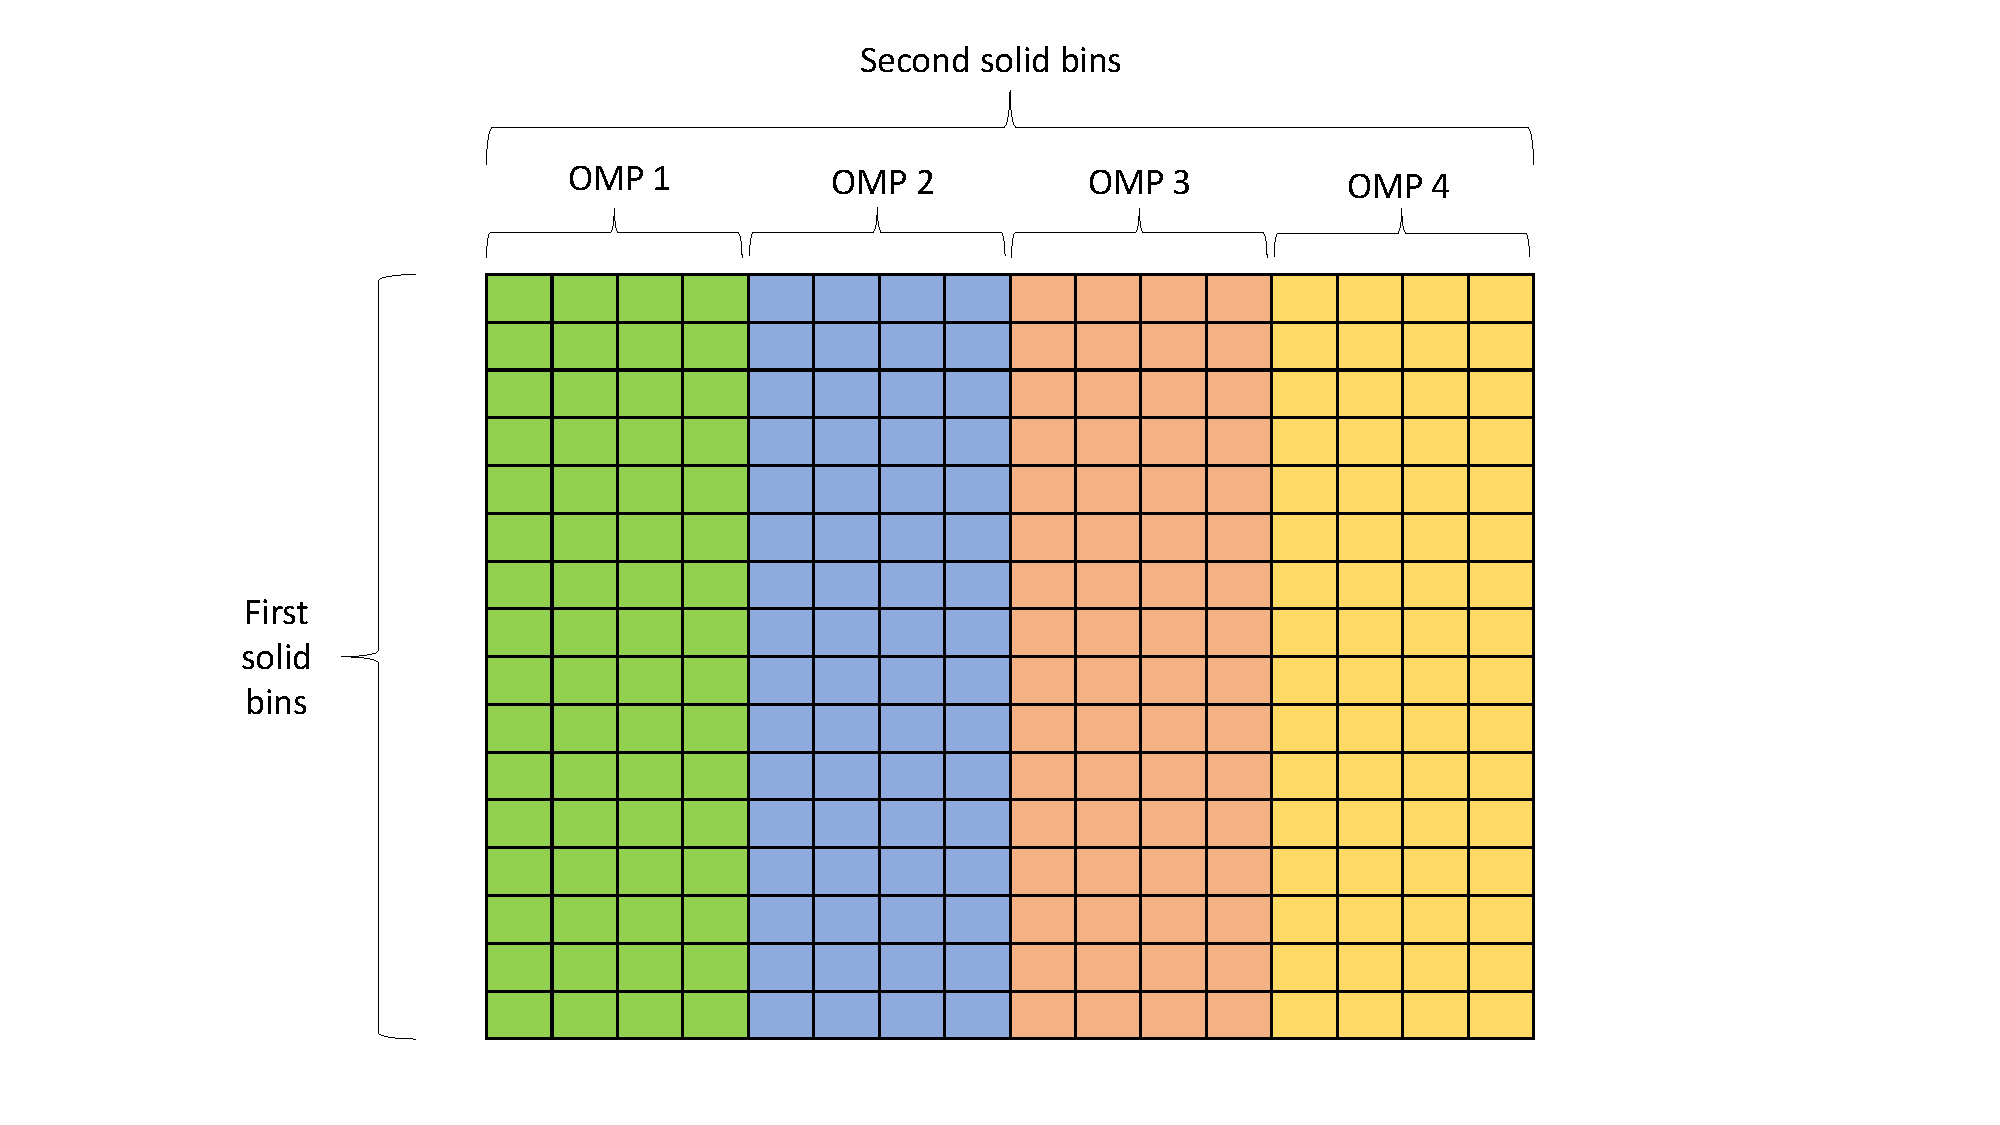
\includegraphics[scale=0.5]{OMP_table.pdf}
\caption{The integration of aggregation rate distributed among OMP processes. This figure indicates the use of 4 OMP processes, the 
configuration that gave us the best performance. This technique has been implemented for each MPI process.}
\label{fig:app_OMP_distribution}
\end{figure}	

\section*{References} 
\bibliographystyle{elsarticle-harv}
\bibliography{Bibli}
\end{document}
